% pdflatex
% chktex-file 1
% chktex-file 8
% chktex-file 13
% chktex-file 38

\documentclass[10pt]{beamer}
\setbeamerfont{frametitle}{size=\large}
\setbeamerfont{block title}{size=\normalsize}
\setbeamerfont{block body}{size=\small}
\setbeamerfont{itemize/enumerate body}{size=\small}
\setbeamerfont{itemize/enumerate subbody}{size=\footnotesize}

\usepackage{PekingU}
% Header样式已修改

\usefonttheme{serif}
%\usepackage[scheme = plain]{ctex}

\usepackage{xcolor}
\usepackage{hyperref}
\hypersetup{
  colorlinks,
  citecolor=blue,
  urlcolor=peking_blue,
  linkcolor=
}
\usepackage{charter} % Nicer fonts

\usepackage{latexsym,amsmath,calligra}
\usepackage{amsfonts} 
\usepackage{bm}

\usepackage{siunitx}
\sisetup{per-mode=symbol}

\usepackage{graphicx}
\usepackage{caption} 
\usepackage{wrapfig}

\usepackage{natbib}

\usepackage{ragged2e}
\usepackage{parskip}
\usepackage{etoolbox}

\usepackage{booktabs}
\usepackage{makecell}
\usepackage{multirow}
\usepackage{multicol}

\usepackage{tikz}
\usetikzlibrary{arrows.meta,calc,positioning,fit}

% Figure placeholder helper: show a framed placeholder if the figure file is missing
\newcommand{\fig}[2]{%
\IfFileExists{#1}{\includegraphics[width=#2]{#1}}{%
\fbox{\parbox[c][0.32\textheight][c]{0.92\linewidth}{\centering
\small Placeholder figure file not found:\\ \texttt{#1}}}}}

\apptocmd{\frame}{}{\justifying}{} % Justify text in all frames.

\newcommand{\theHalgorithm}{\arabic{algorithm}}
\theoremstyle{plain}
\newtheorem{axiom}{Axiom}
\newtheorem{claim}[axiom]{Claim}
\newtheorem{assumption}{Assumption}
\newtheorem{remark}{Remark}
\newtheorem{proposition}{Proposition}
\setbeamertemplate{theorems}[numbered] 


\author[Feng, Liu \& Hu]{Yizhan Feng \and Tianle Liu \and Jiahao Hu}
\title[PDAC Proteomic Biomarkers]{Prospective observational study on biomarkers of response in pancreatic ductal adenocarcinoma}
\institute{Yuanpei College, Peking University}
\date{2025/12/24}

% Define a conditional to control whether to show the logo globally
\newif\ifplacelogo
\placelogotrue % Enable logo globally
% Set global logo (can be empty if \placelogofalse)
\logo{%
  \ifplacelogo
    \includegraphics[width=2cm]{../Figures/PKU-China-logo.png}%
  \fi
}

% official colors match with the PKU red
\def\cmd#1{\texttt{\color{red}\footnotesize \(\backslash\)#1}}
\def\env#1{\texttt{\color{blue}\footnotesize #1}}
\definecolor{deepblue}{rgb}{0,0,0.5}
\definecolor{deepred}{rgb}{0.6,0,0}
\definecolor{deepgreen}{rgb}{0,0.5,0}
\definecolor{halfgray}{gray}{0.55}

\begin{document}
{
\setbeamertemplate{logo}{}
\begin{frame}
    \titlepage
    \begin{figure}[htpb]
        \begin{center}
            
\includegraphics[width=0.2\linewidth]{Figures/PKUlogo.png}
        \end{center}
    \end{figure}
\end{frame}
}

\placelogofalse

\section{Literature Information}

\begin{frame}{Literature Information}
  \begin{columns}[T,onlytextwidth]
    \begin{column}{0.5\textwidth}
      \vspace{-0.5cm}
      
\includegraphics[width=\linewidth]{Figures/Cover.jpg}
      \small{
      \textit{Nature Medicine}, 30, 749–761 (2024).

      DOI: 10.1038/s41591-023-02790-x
      }
    \end{column}
    \begin{column}{0.5\textwidth}
      \vspace{0pt}
      \small
      \textbf{Title}\\
      Prospective observational study on biomarkers of response in pancreatic ductal adenocarcinoma
      \\[0.5cm]
      \textbf{Study at a glance}
      \begin{itemize}
        \item Tissue proteomics map with \textbf{32 functional protein modules}
        \item \textbf{14-protein} LASSO-Cox prognostic score (OS/DFS stratification)
        \item Two predictive biomarkers for adjuvant chemotherapy benefit: \textbf{NDUFB8} and \textbf{CEMIP2}
        \item External/extended validation for chemo-benefit biomarkers in \textbf{3 independent cohorts}.
      \end{itemize}
    \end{column}
  \end{columns}
\end{frame}

\section{Research Background}

\begin{frame}{Background \& Difficulty}
  \textbf{Fact}
  \begin{itemize}
    \item Pancreatic ductal adenocarcinoma (PDAC), one of the deadliest solid malignancies, is estimated to become the second-leading cause of cancer-related mortality by 2030.
    \item Most patients present advanced disease at diagnosis, owing to a lack of effective disease screening.
    \item Even with intensive adjuvant chemotherapy, recurrence rates remain extremely high, reaching 69--75\% within 2 years.
    \item The cost associated with RNA-based signatures, reliant on high-throughput sequencing, remains prohibitive compared to immunohistochemistry (IHC) biomarkers.
  \end{itemize}

  \vspace{0.4em}

  \textbf{Core difficulty}
  \begin{itemize}
    \item Postoperative chemotherapy is a standard therapy, but its therapeutic effect is poor for some patients. For some patients it is life-saving; for others it may be ineffective.
  \end{itemize}
\end{frame}


\begin{frame}{Research objective}
  \begin{center}
  \Large Can we predict which kind of patients will achieve good therapeutic effects, through measurable biomarkers?
  \end{center}

  \vspace{1.4em}

  \centering
  \resizebox{0.7\textwidth}{!}{
  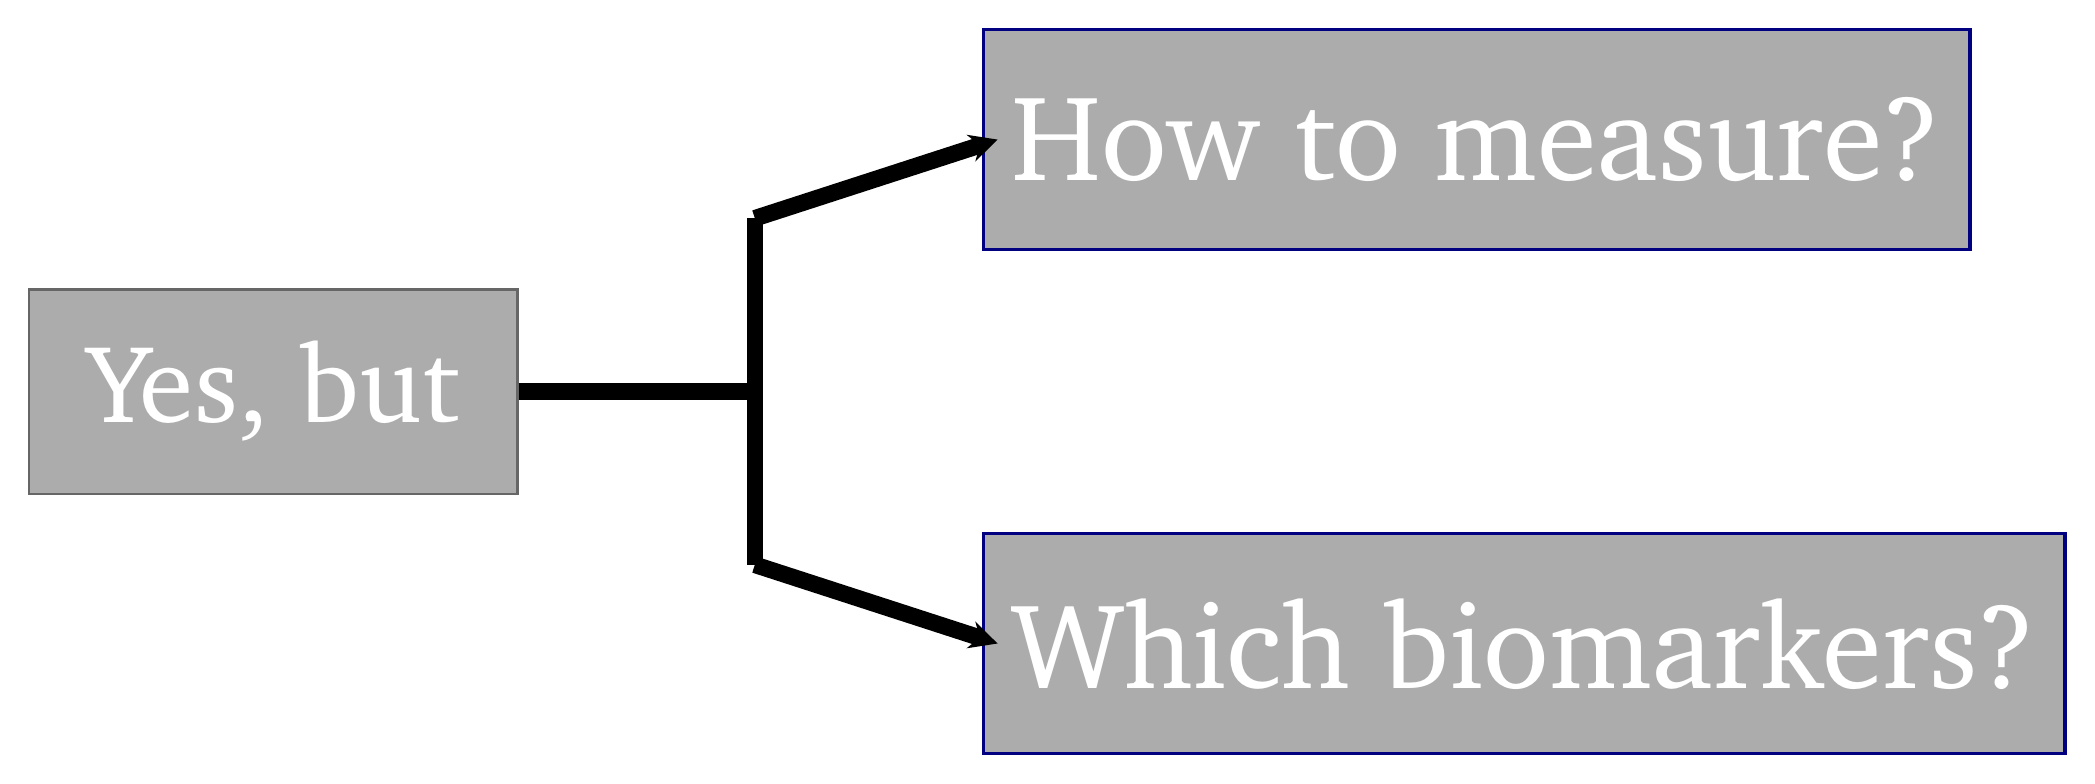
\begin{tikzpicture}[
    boxL/.style={
      draw=black!60, line width=1pt,
      fill=gray!65,
      minimum width=6.2cm, minimum height=2.6cm,
      text=white,
      font=\rmfamily\fontsize{40}{40}\selectfont,
      inner sep=10pt
    },
    boxR/.style={
      draw=blue!50!black, line width=1.2pt,
      fill=gray!65,
      minimum width=10.2cm, minimum height=2.8cm,
      text=white,
      font=\rmfamily\fontsize{44}{44}\selectfont,
      inner sep=10pt
    },
    conn/.style={line width=6pt, draw=black},
    arr/.style={-{Stealth[length=10pt,width=10pt]}, line width=6pt, draw=black}
  ]

  % Nodes
  \node[boxL] (L) at (0,0) {Yes, but};

  \node[boxR, anchor=west] (T) at (9, 3.2) {How to measure?};
  \node[boxR, anchor=west] (B) at (9,-3.2) {Which biomarkers?};

  % Key coordinates for the bracket connector
  \coordinate (J) at ($(L.east)+(3.0,0)$);          % junction point (trunk x)
  \coordinate (Vtop) at ($(J)+(0,2.2)$);
  \coordinate (Vbot) at ($(J)+(0,-2.2)$);

  % Left horizontal connector into the trunk
  \draw[conn] (L.east) -- (J);

  % Vertical trunk
  \draw[conn] (Vbot) -- (Vtop);

  % Top branch + arrow into top box
  \draw[conn] (J) -- (Vtop);
  \draw[arr]  (Vtop) -- ($(T.west)+(0.2,0)$);

  % Bottom branch + arrow into bottom box
  \draw[conn] (J) -- (Vbot);
  \draw[arr]  (Vbot) -- ($(B.west)+(0.2,0)$);

  \end{tikzpicture}
  }
\end{frame}


\section{Research Methods \& Results}

\begin{frame}{Protein screening: proteomics approach}
  \begin{columns}[onlytextwidth]
    \begin{column}{0.5\textwidth}
      \begin{itemize}
        \item Extract all proteins from Tumor and TAT (Tumor Adjacent Tissue), quantify the types and abundance of proteins in different tissues by mass spectrometry, and then use statistical methods for separation, such as principal component analysis (PCA), etc.
        \item This study analyzed 191 tumors and 90 normal tissues, generating a detailed list of nearly 8,000 proteins.
      \end{itemize}
    \end{column}

    \begin{column}{0.45\textwidth}
        \begin{figure}
          \begin{center}
            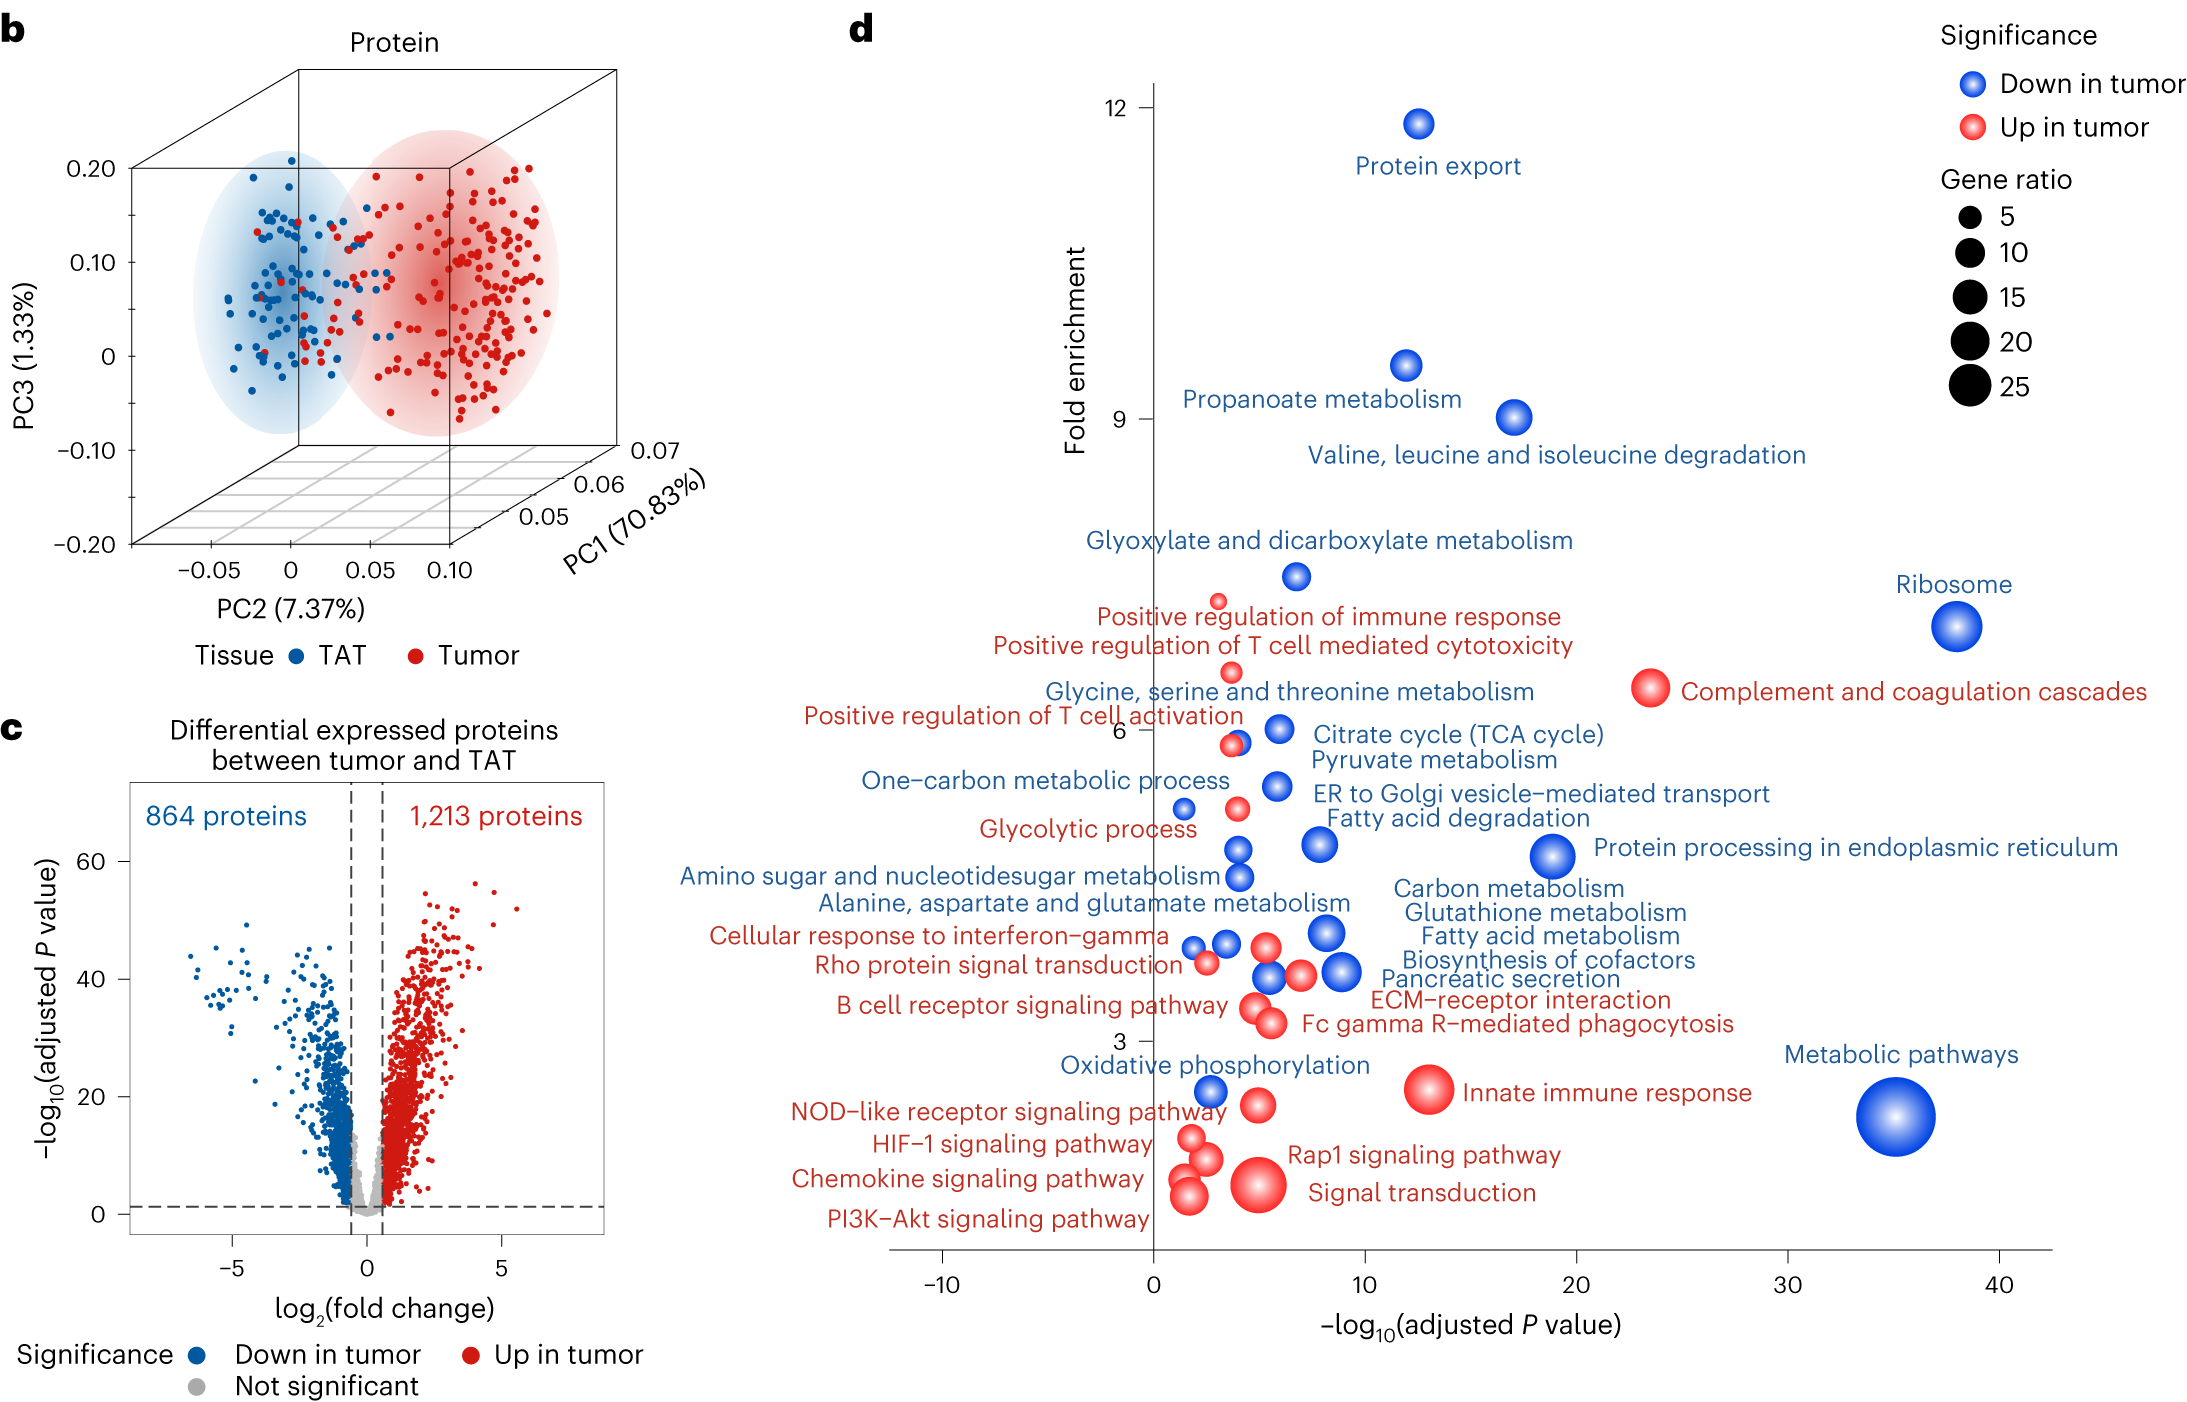
\includegraphics[width=\linewidth]{Figures/Fig1b-d.png}
          \end{center}
          \caption{Protein screening}
        \end{figure}
    \end{column}
  \end{columns}
  
  \begin{itemize}
    \item By comparison, we can identify which proteins are significantly differentially expressed in tumor cells, and further screen potential biomarkers related to benefit from adjuvant chemotherapy.
  \end{itemize}
\end{frame}

\begin{frame}{Figure \& Code}
  \begin{columns}[T,onlytextwidth]
    \begin{column}{0.5\textwidth}
        \begin{figure}
          \begin{center}
            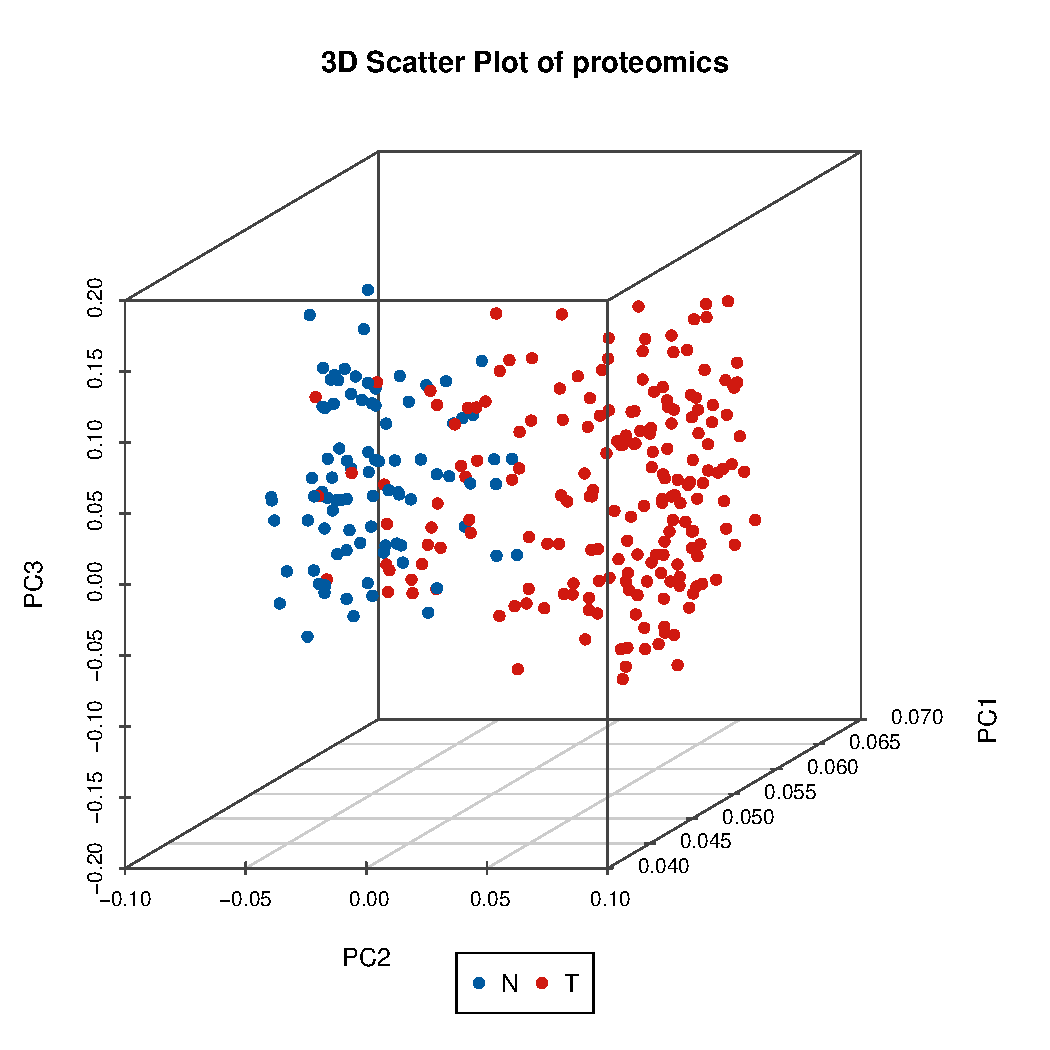
\includegraphics[width=0.9\linewidth]{Figures/1B.PRO_PCA3d.pdf}
          \end{center}
        \end{figure}
    \end{column}

    \begin{column}{0.5\textwidth}
        \begin{figure}
          \begin{center}
            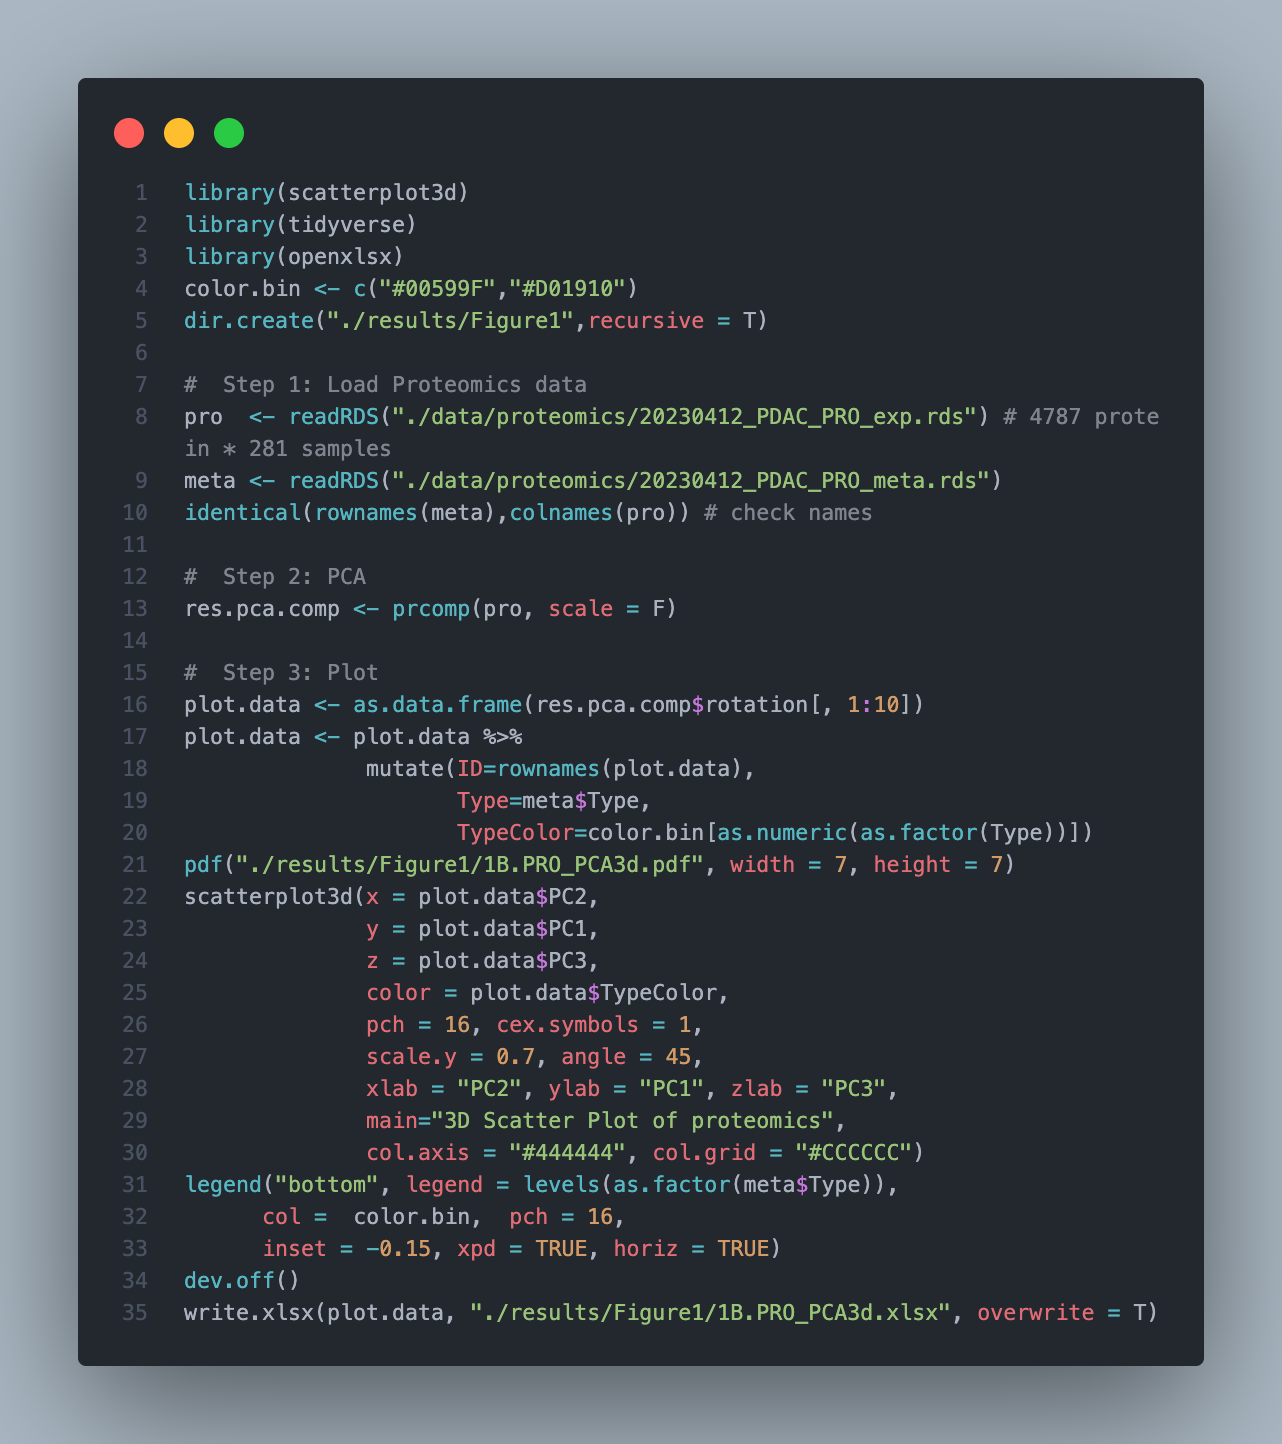
\includegraphics[width=0.9\linewidth]{Figures/1B.PRO_PCA3d-code.png}
          \end{center}
        \end{figure}
    \end{column}
  \end{columns}

  \vspace{0.5cm}
  Principal-component analyses (PCAs) involving 4,787 analyzable proteins revealed a clear separation between tumors and TACs.
\end{frame}

\begin{frame}{Figure \& Code}
  \begin{columns}[T,onlytextwidth]
    \begin{column}{0.6\textwidth}
        \begin{figure}
          \begin{center}
            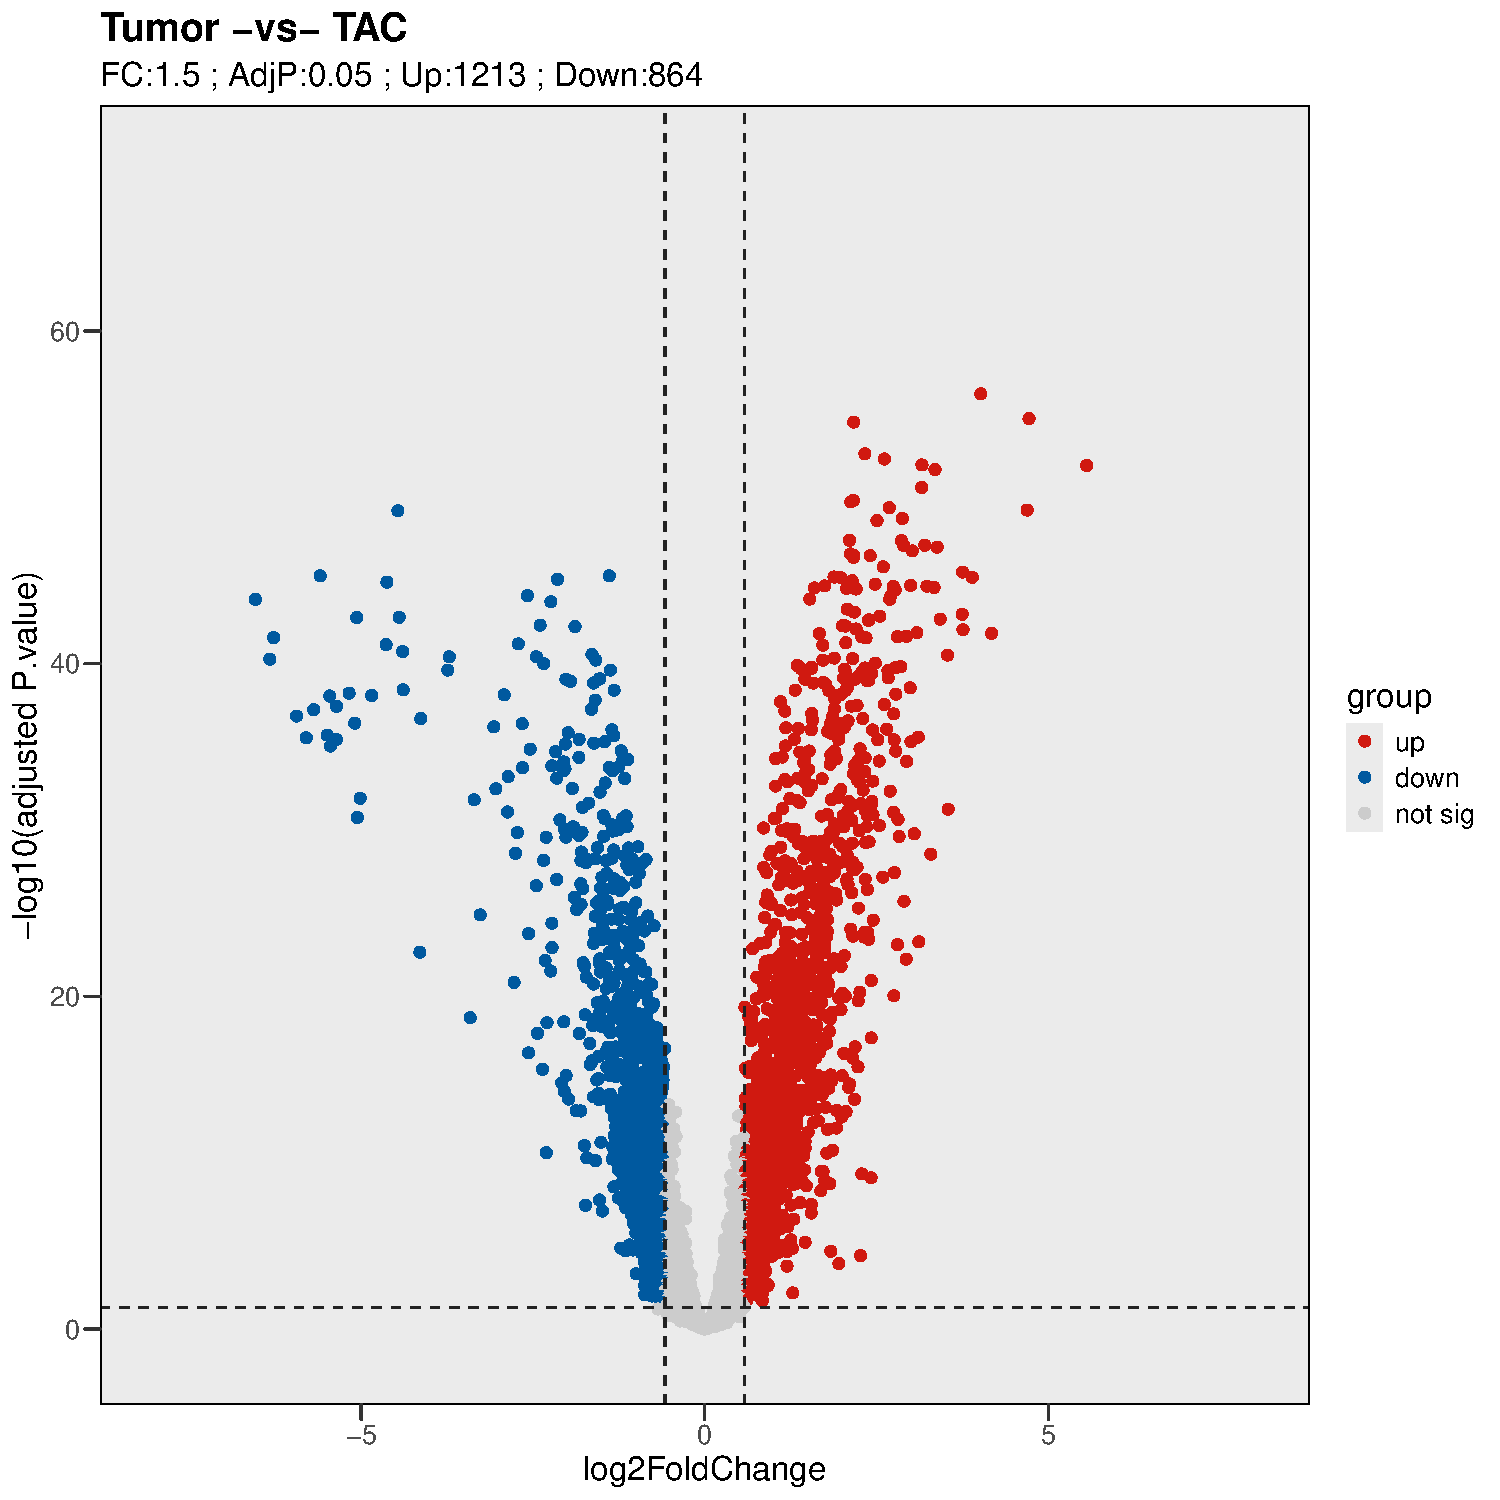
\includegraphics[width=0.9\linewidth]{Figures/1C.PRO_Limma_fc1.5.pdf}
          \end{center}
        \end{figure}
    \end{column}

    \begin{column}{0.4\textwidth}
        \begin{figure}
          \begin{center}
            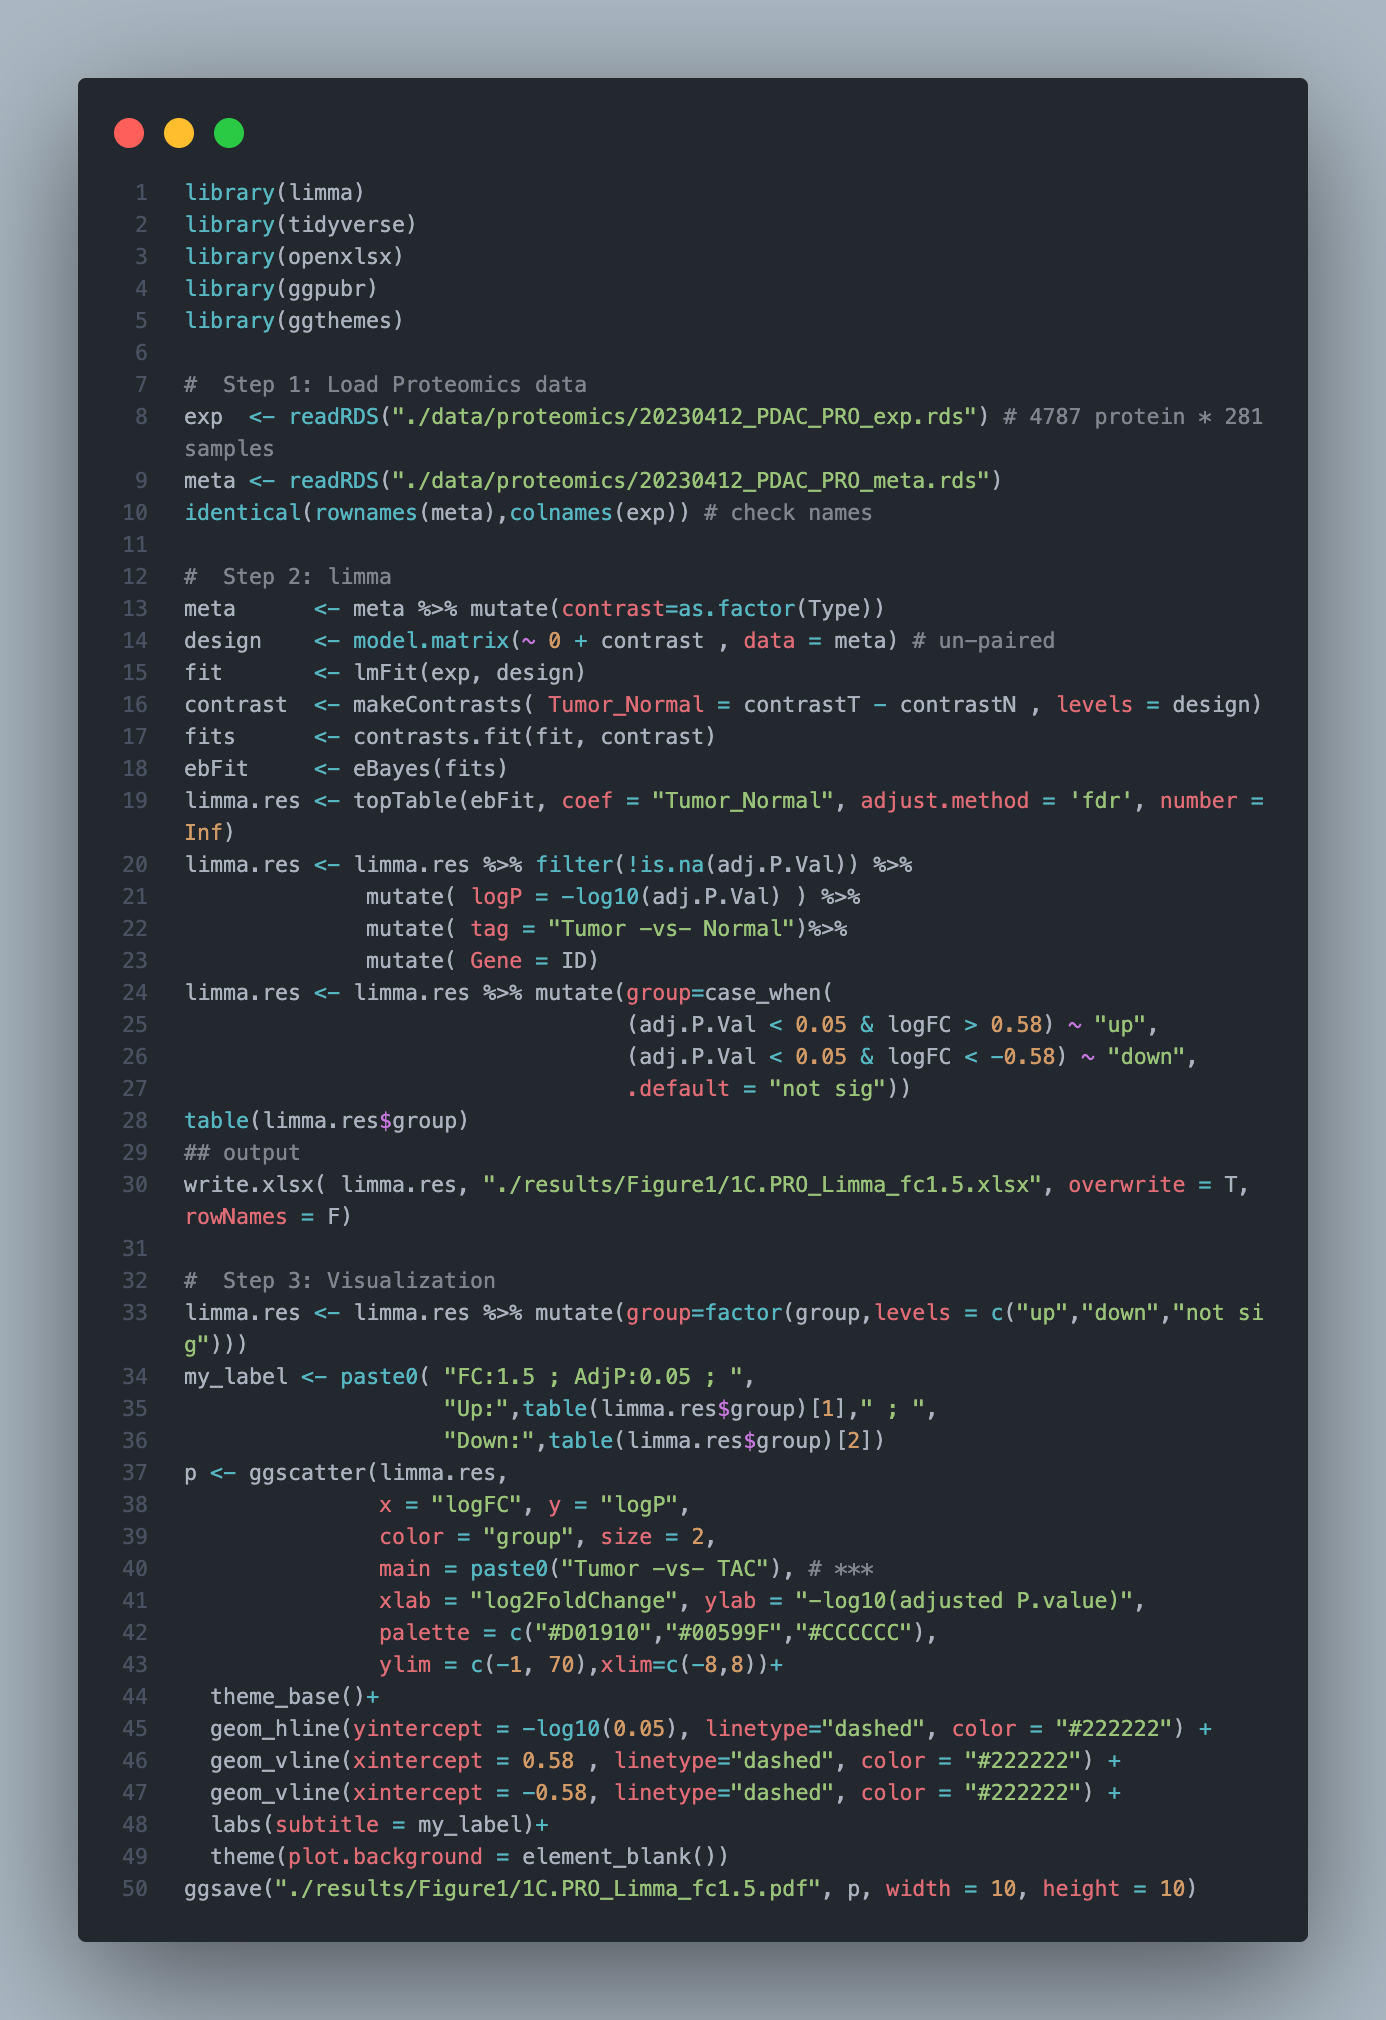
\includegraphics[width=0.9\linewidth]{Figures/1C.PRO_Limma_fc1.5-code.png}
          \end{center}
        \end{figure}
    \end{column}
  \end{columns}

  \vspace{0.5cm}
  Volcano plot displaying differentially expressed proteins between tumors and TACs, with 1,213 proteins significantly up-regulated and 864 proteins down-regulated in tumors as compared to TACs.
\end{frame}

\begin{frame}{Figure \& Code}
  \begin{columns}[T,onlytextwidth]
    \begin{column}{0.55\textwidth}
        \begin{figure}
          \begin{center}
            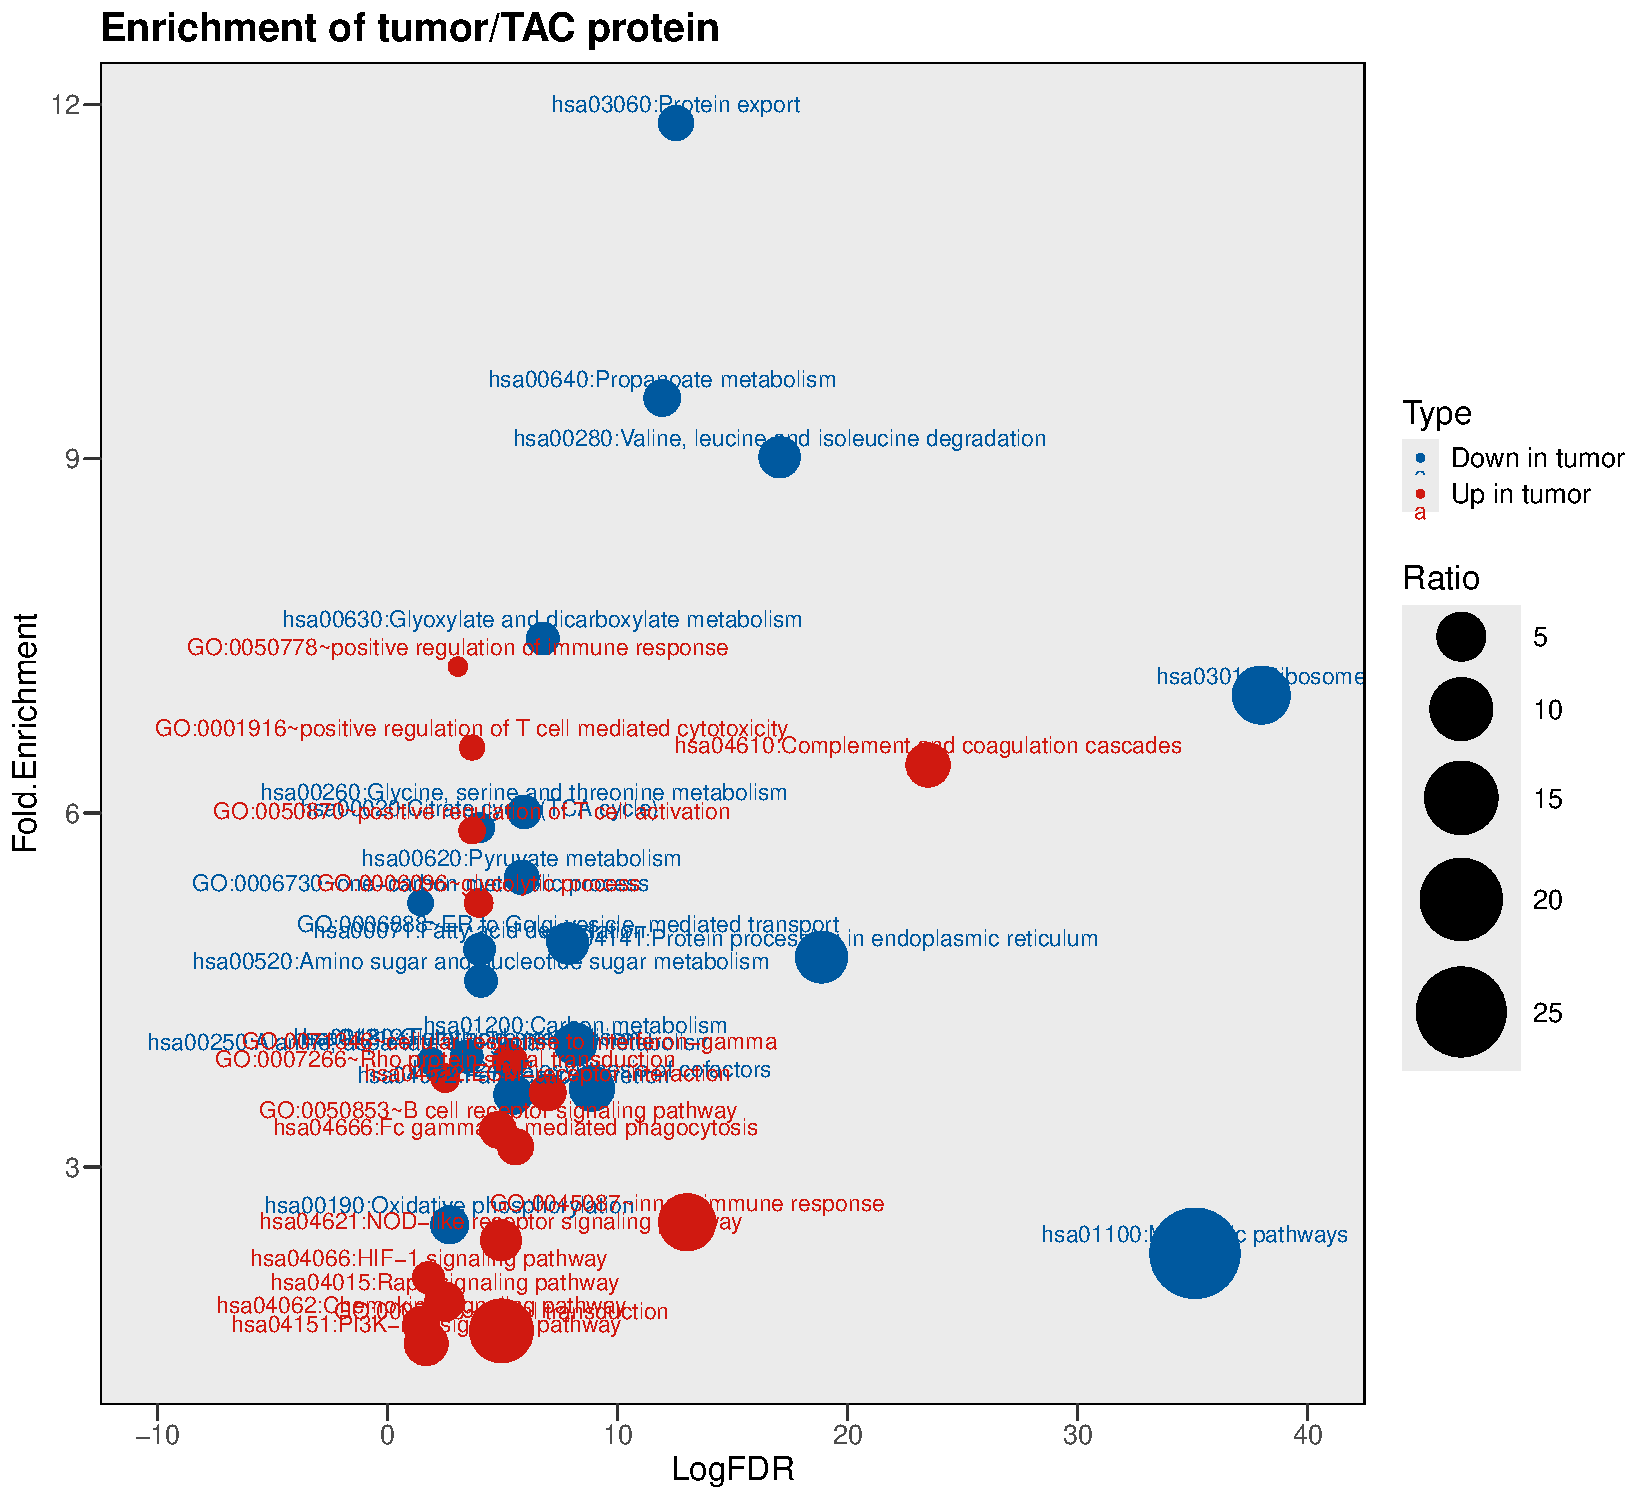
\includegraphics[width=0.9\linewidth]{Figures/1D.PRO_deg.tn_enrich.pdf}
          \end{center}
        \end{figure}
    \end{column}

    \begin{column}{0.45\textwidth}
        \begin{figure}
          \begin{center}
            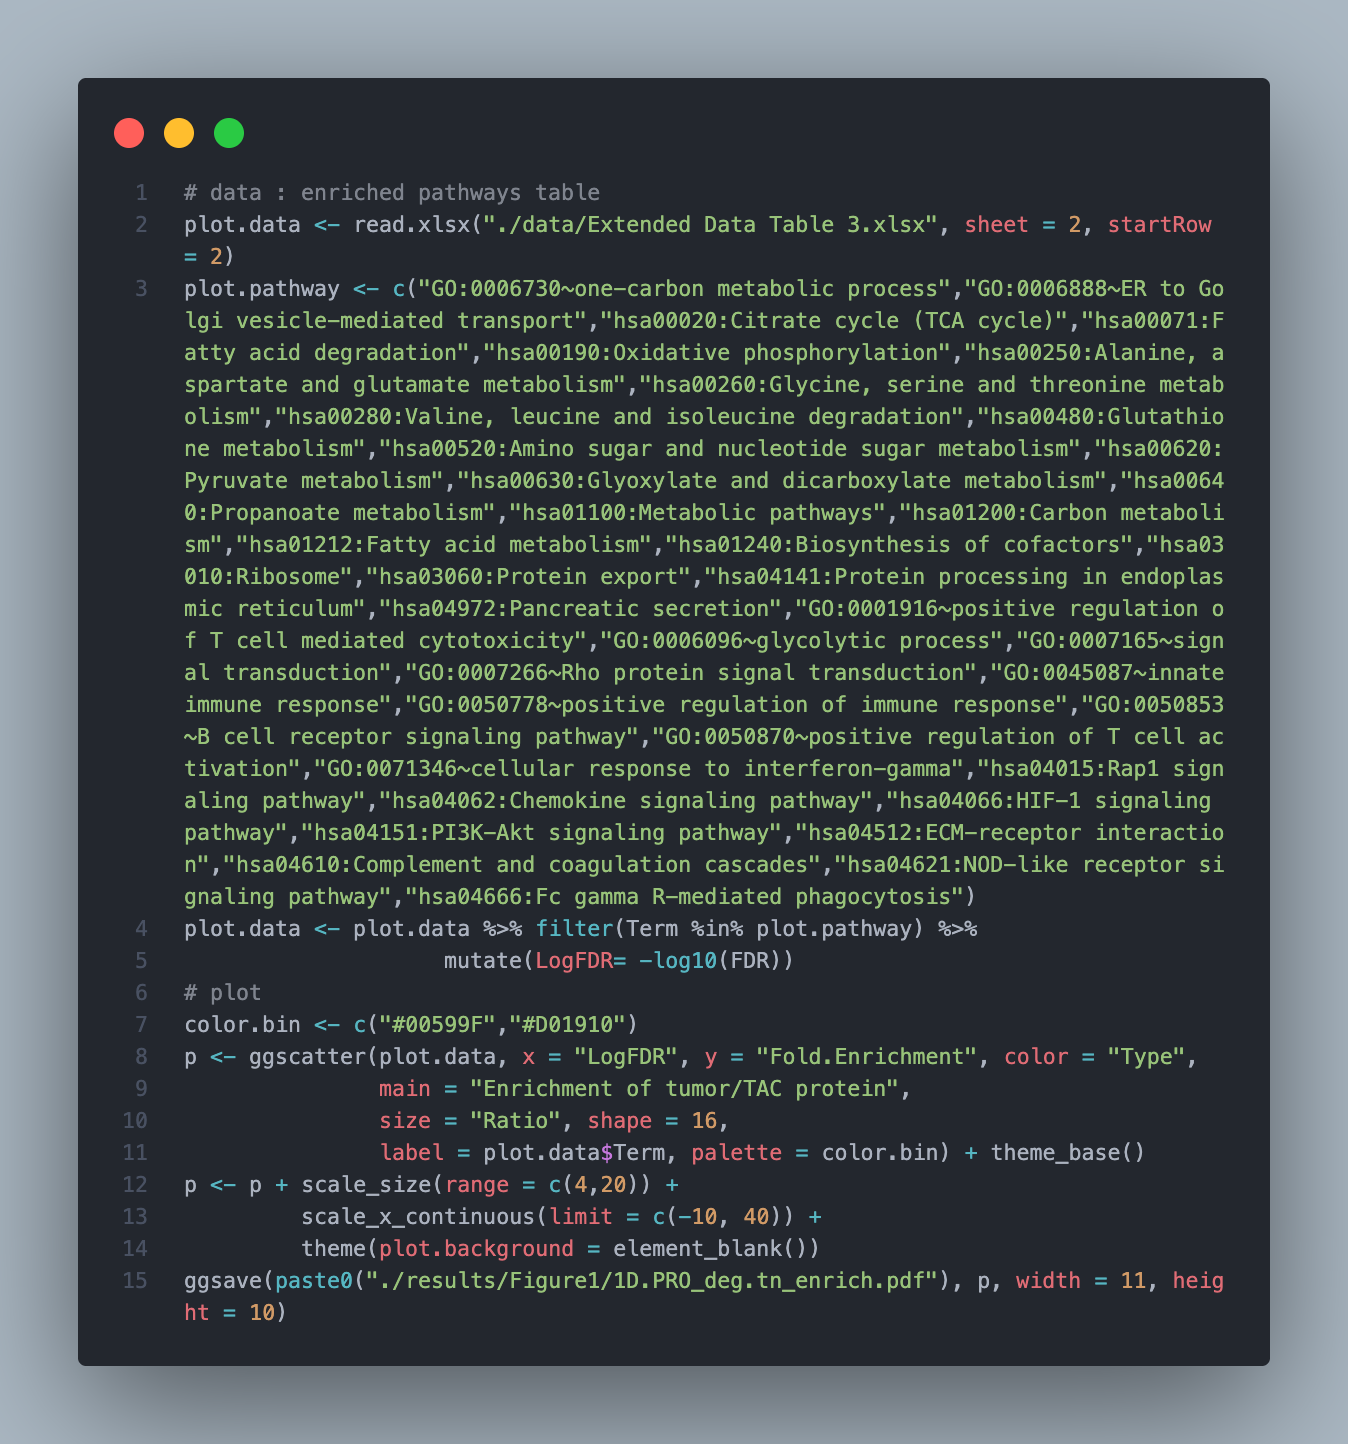
\includegraphics[width=0.9\linewidth]{Figures/1D.PRO_deg.tn_enrich-code.png}
          \end{center}
        \end{figure}
    \end{column}
  \end{columns}

  \vspace{0.5cm}
  Dot plot illustrating enriched pathways identified based on significantly up/down-regulated proteins. Red dots represent pathways enriched (adjusted P-value $<$ 0.05) for proteins up-regulated in tumors compared to TACs, while blue dots represent pathways enriched (adjusted P-value $<$ 0.05) for proteins down-regulated in tumors.
\end{frame}

\begin{frame}{Clustering-based screening: WGCNA}
  \begin{columns}[onlytextwidth]
    \begin{column}{0.5\textwidth}
      \begin{itemize}
        \item WGCNA: Weighted Correlation Network Analysis
        \item  We cannot analyze about 8,000 proteins one by one, so we use WGCNA to group proteins with consistent behavior (co-upregulated or co-downregulated) into the same category.
        \item In total, 32 stable functional protein modules were identified for downstream analysis.
      \end{itemize}
    \end{column}

    \begin{column}{0.45\textwidth}
        \begin{figure}
          \begin{center}
            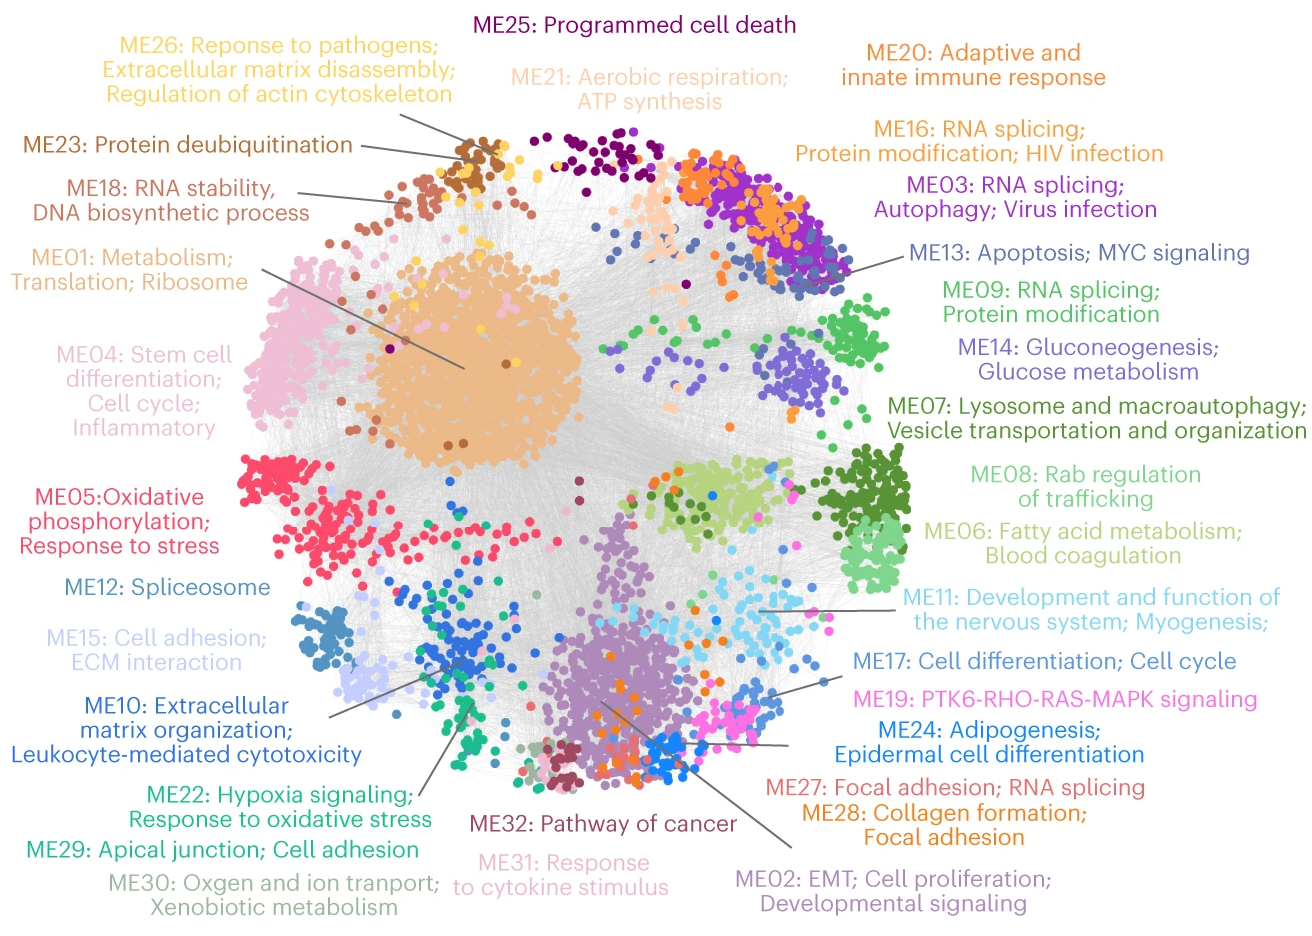
\includegraphics[width=\linewidth]{Figures/Fig2a.png}
          \end{center}
          \caption{WGCNA}
        \end{figure}
    \end{column}
  \end{columns}  
\end{frame}

\begin{frame}{Weighted Correlation Network Analysis}
  \begin{figure}
    \begin{center}
      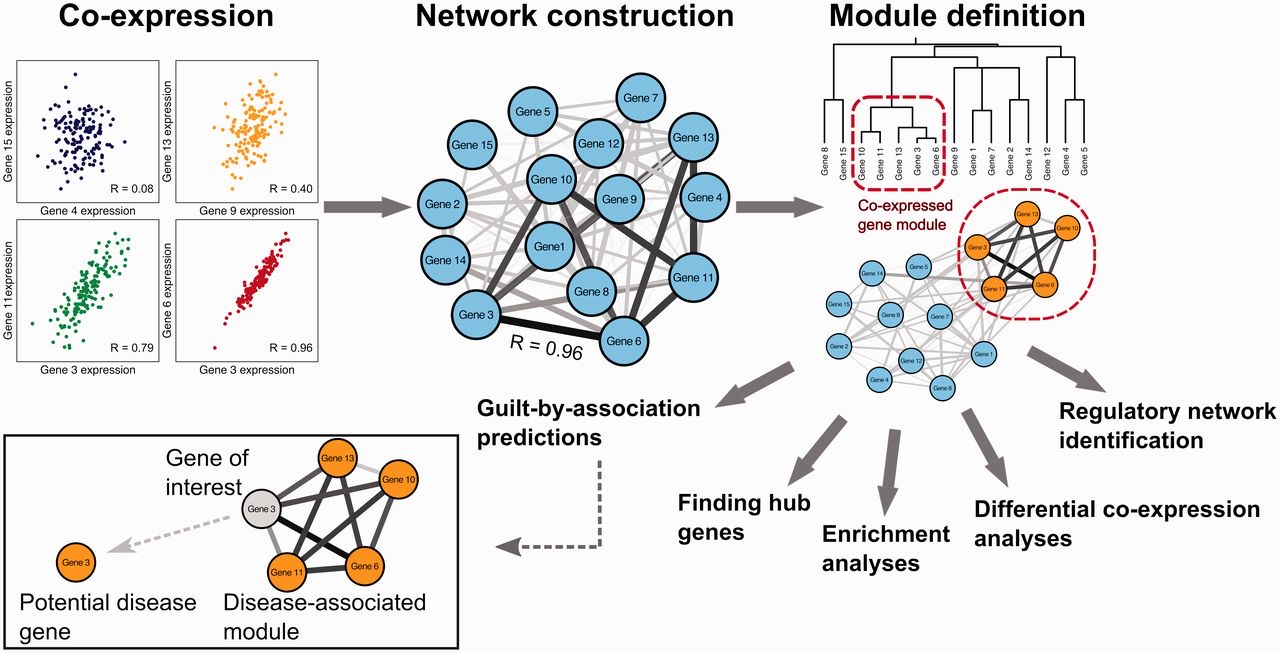
\includegraphics[width=\linewidth]{Figures/WGCNA.JPEG}
    \end{center}
    \caption{Weighted Correlation Network Analysis}
  \end{figure}
\end{frame}

\begin{frame}{Figure \& Code}
  \begin{columns}[onlytextwidth]
    \begin{column}{0.55\textwidth}
        \begin{figure}
          \begin{center}
            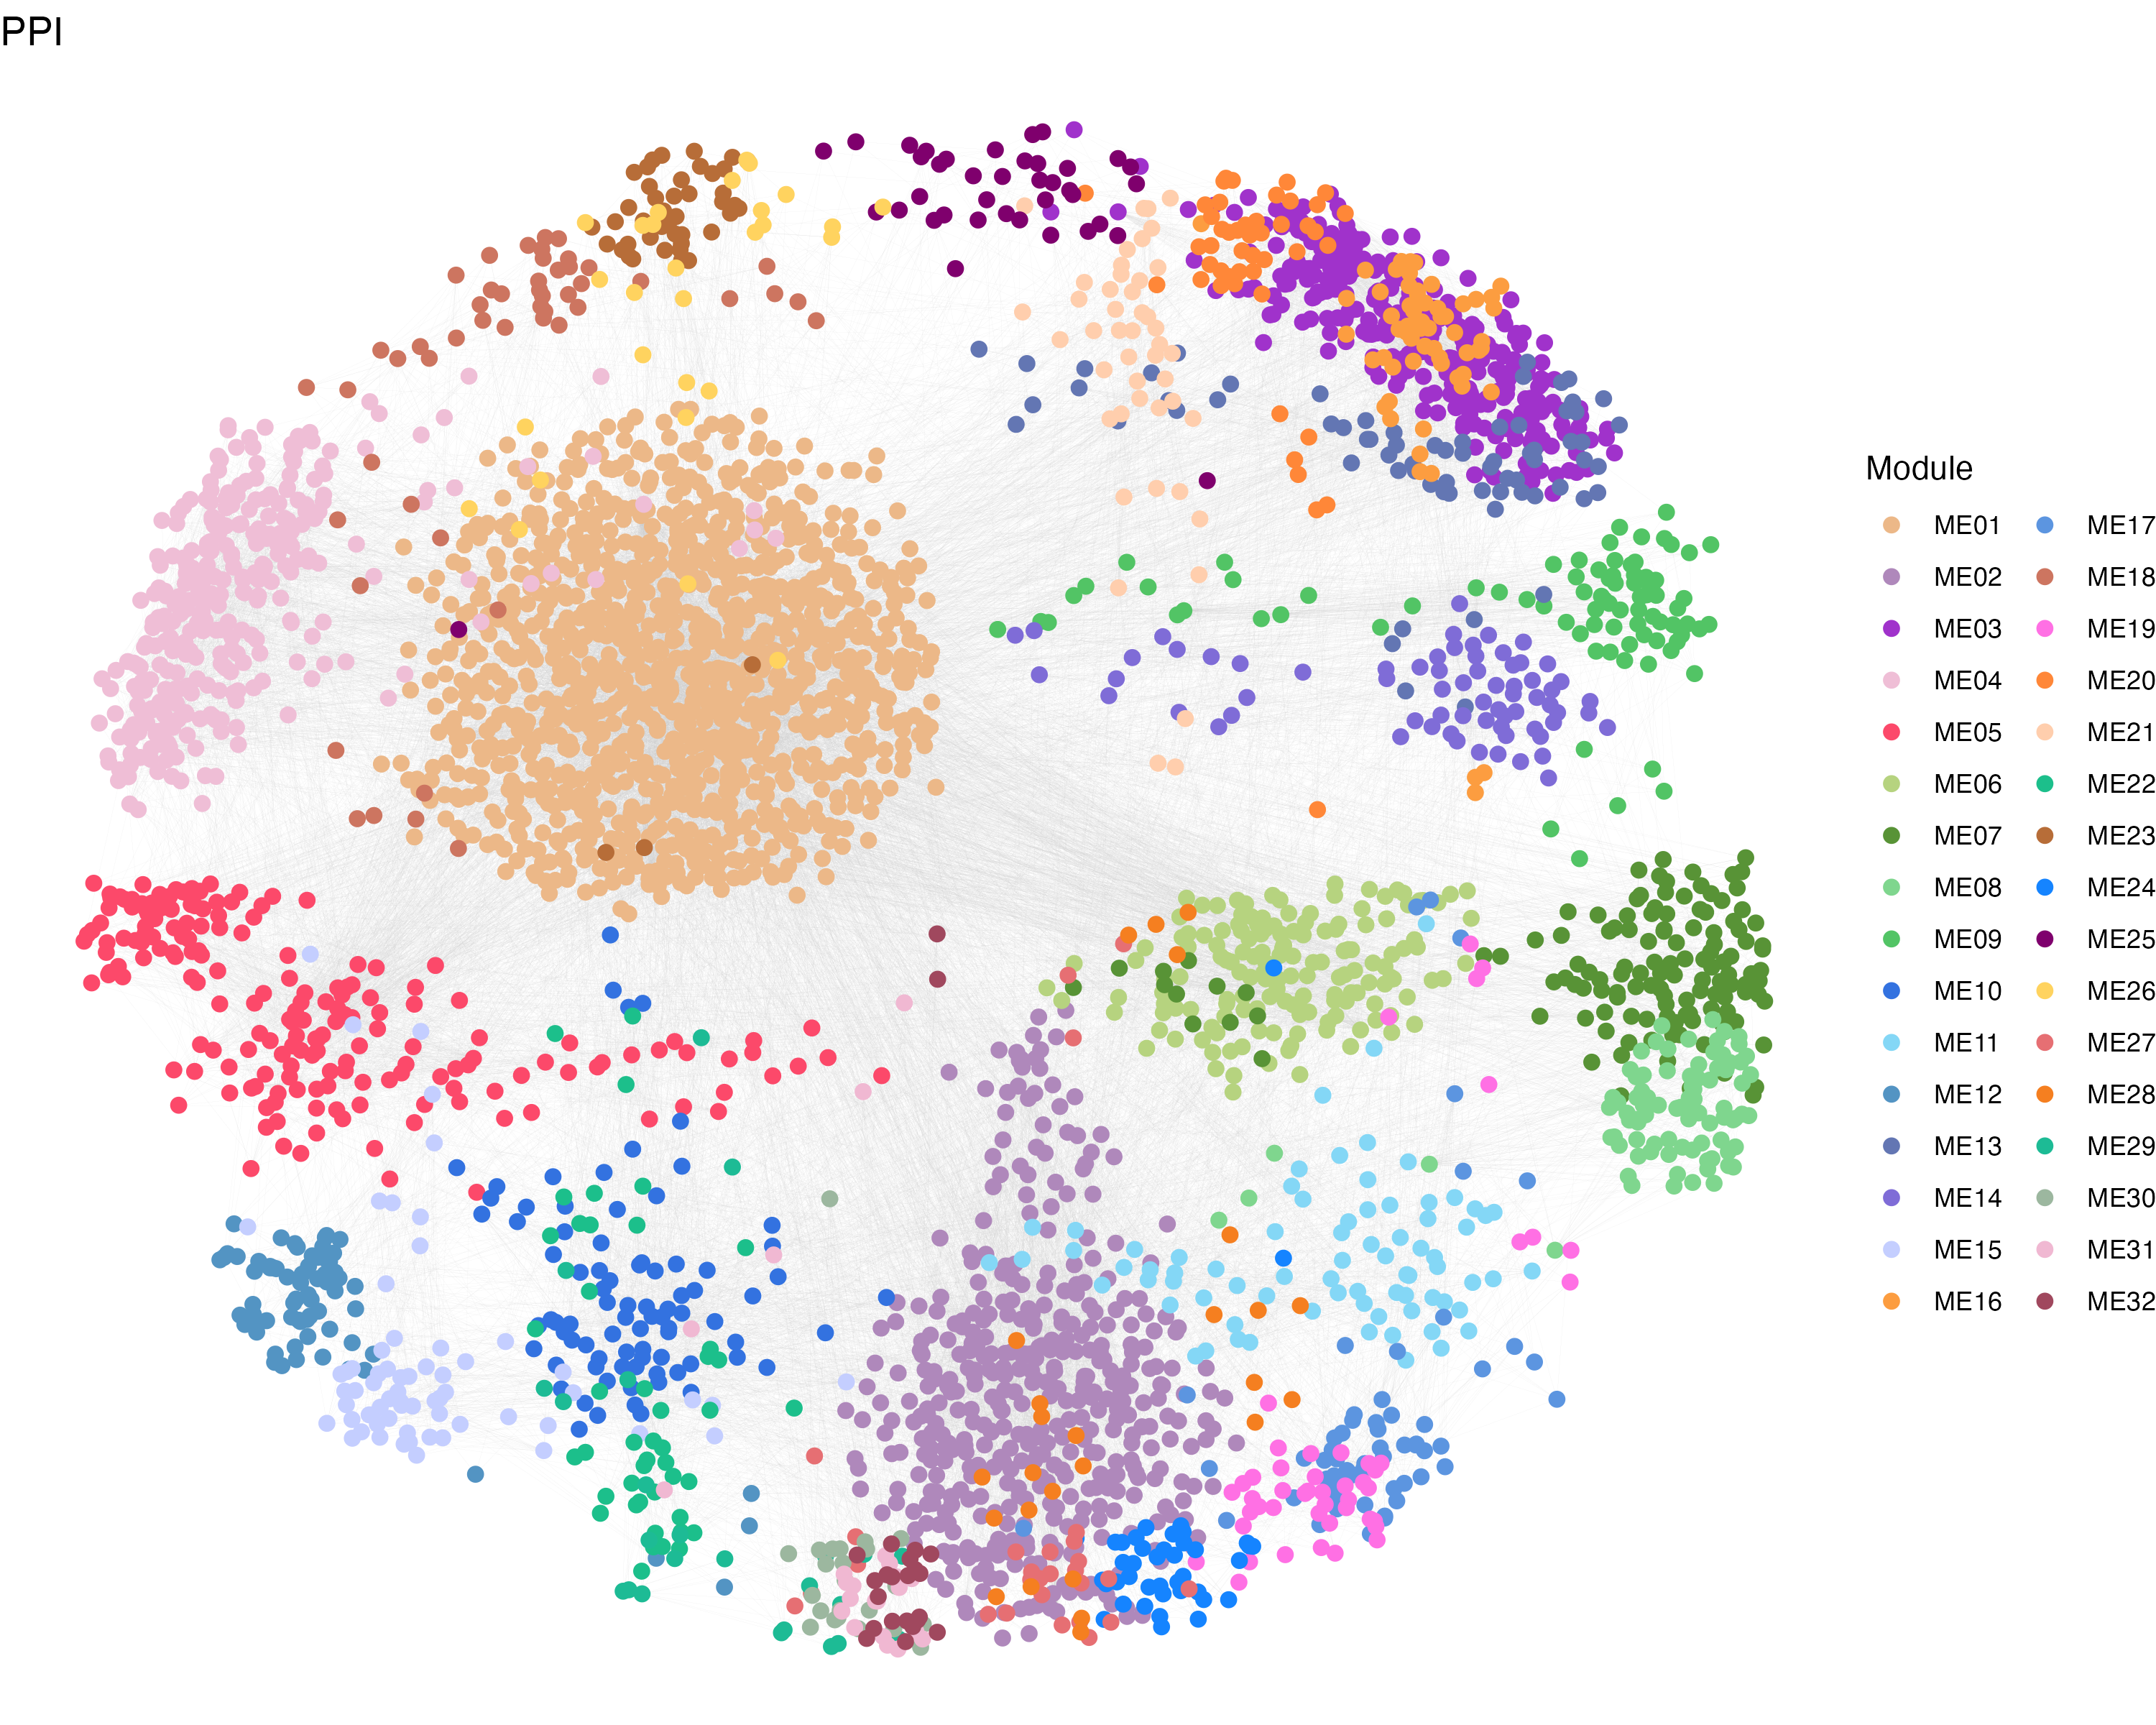
\includegraphics[width=0.9\linewidth]{Figures/2A-PRO-modules.png}
          \end{center}
        \end{figure}
    \end{column}

    \begin{column}{0.45\textwidth}
        \begin{figure}
          \begin{center}
            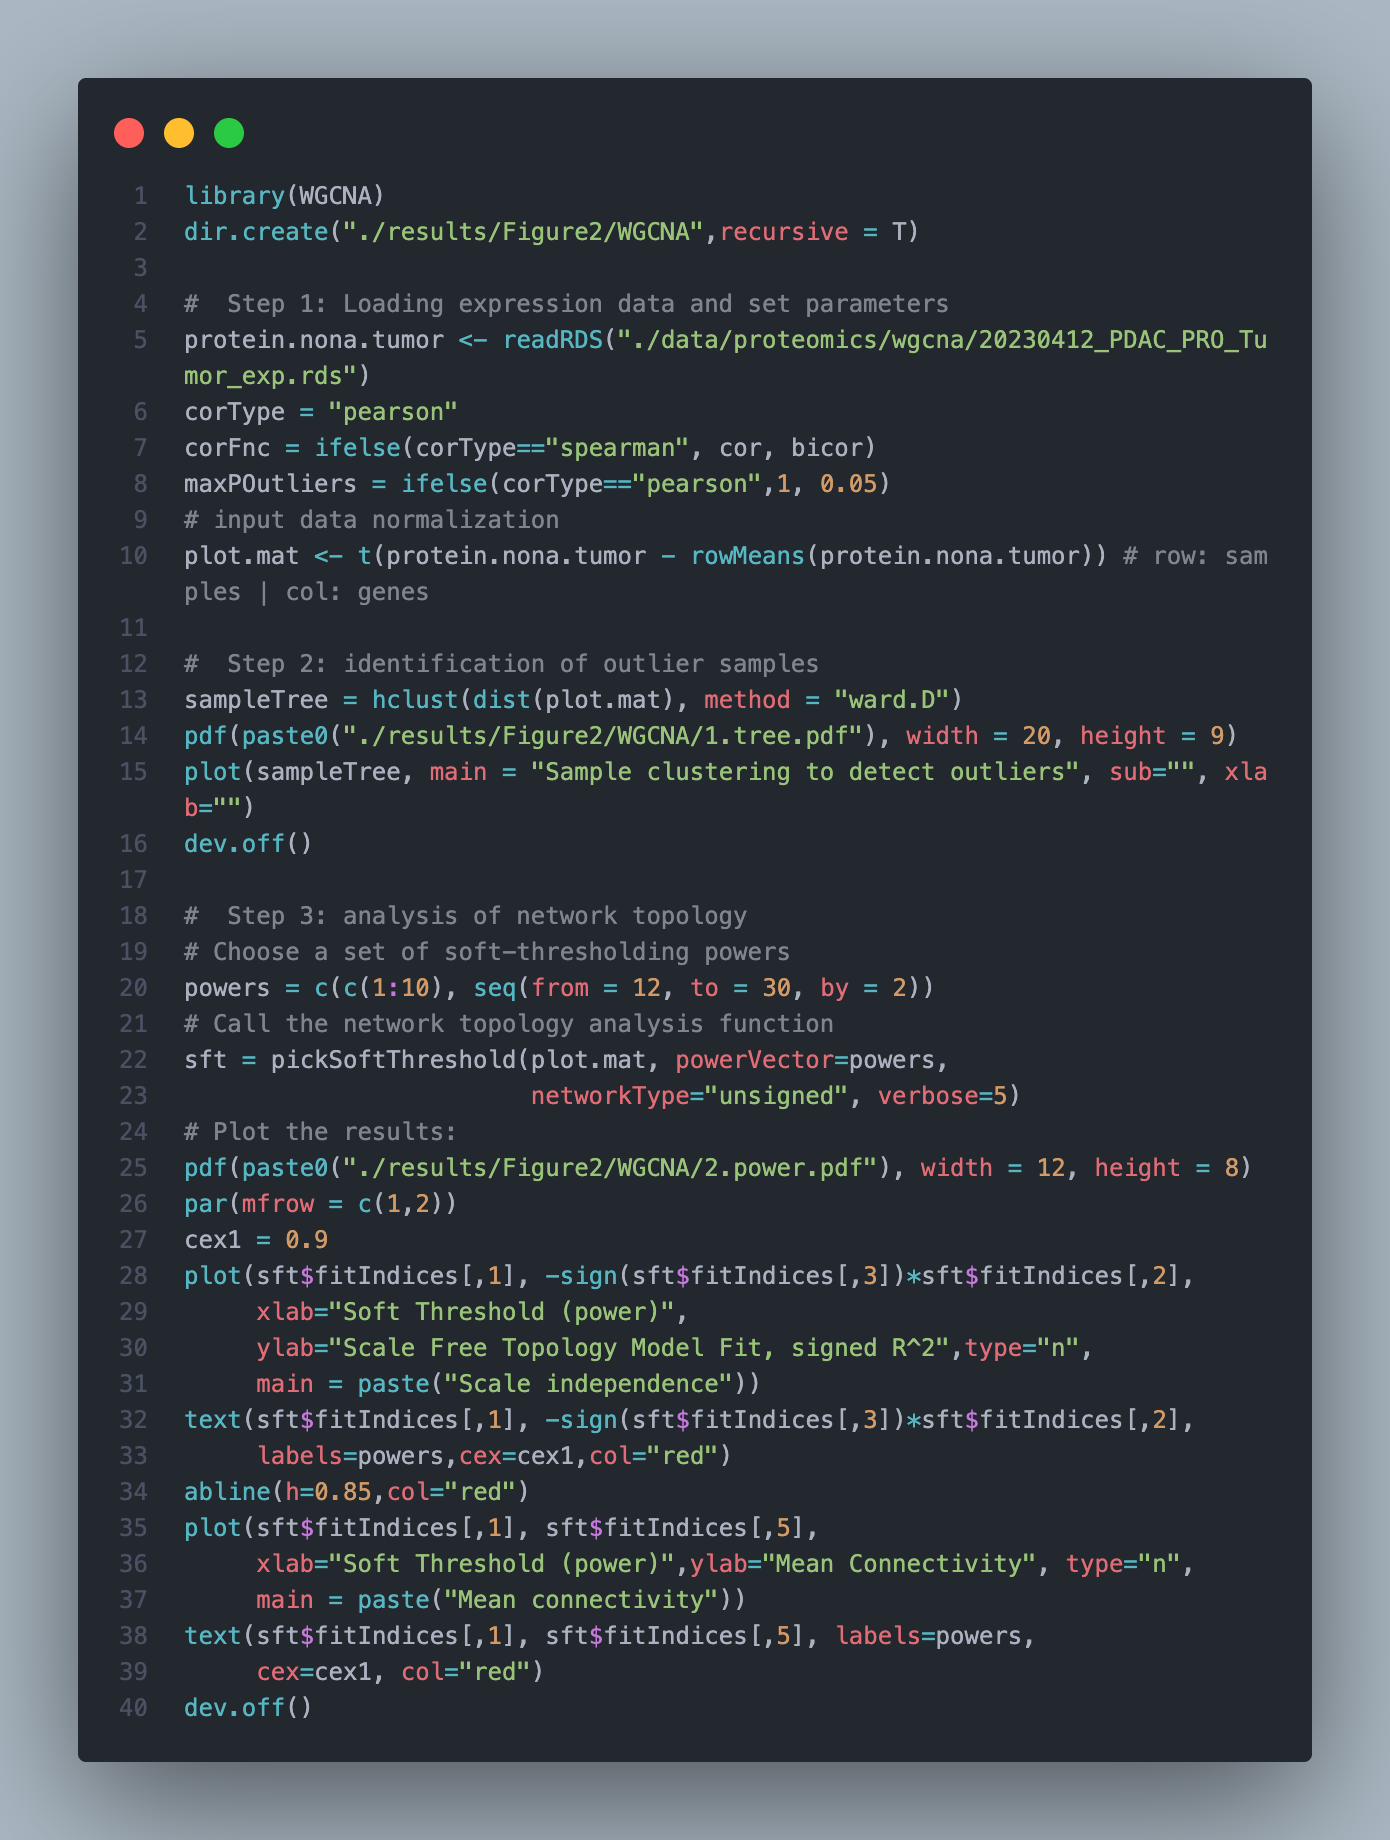
\includegraphics[width=0.9\linewidth]{Figures/2A-PRO-modules-code1.png}
          \end{center}
        \end{figure}
    \end{column}
  \end{columns}
 
  \vspace{0.5cm}
  We performed weighted correlation network analysis WGCNA on proteomic data from tumor samples, identifying a total of 32 functional modules. 
\end{frame}

\begin{frame}{Figure \& Code}
  \begin{columns}[onlytextwidth]
    \begin{column}{0.55\textwidth}
        \begin{figure}
          \begin{center}
            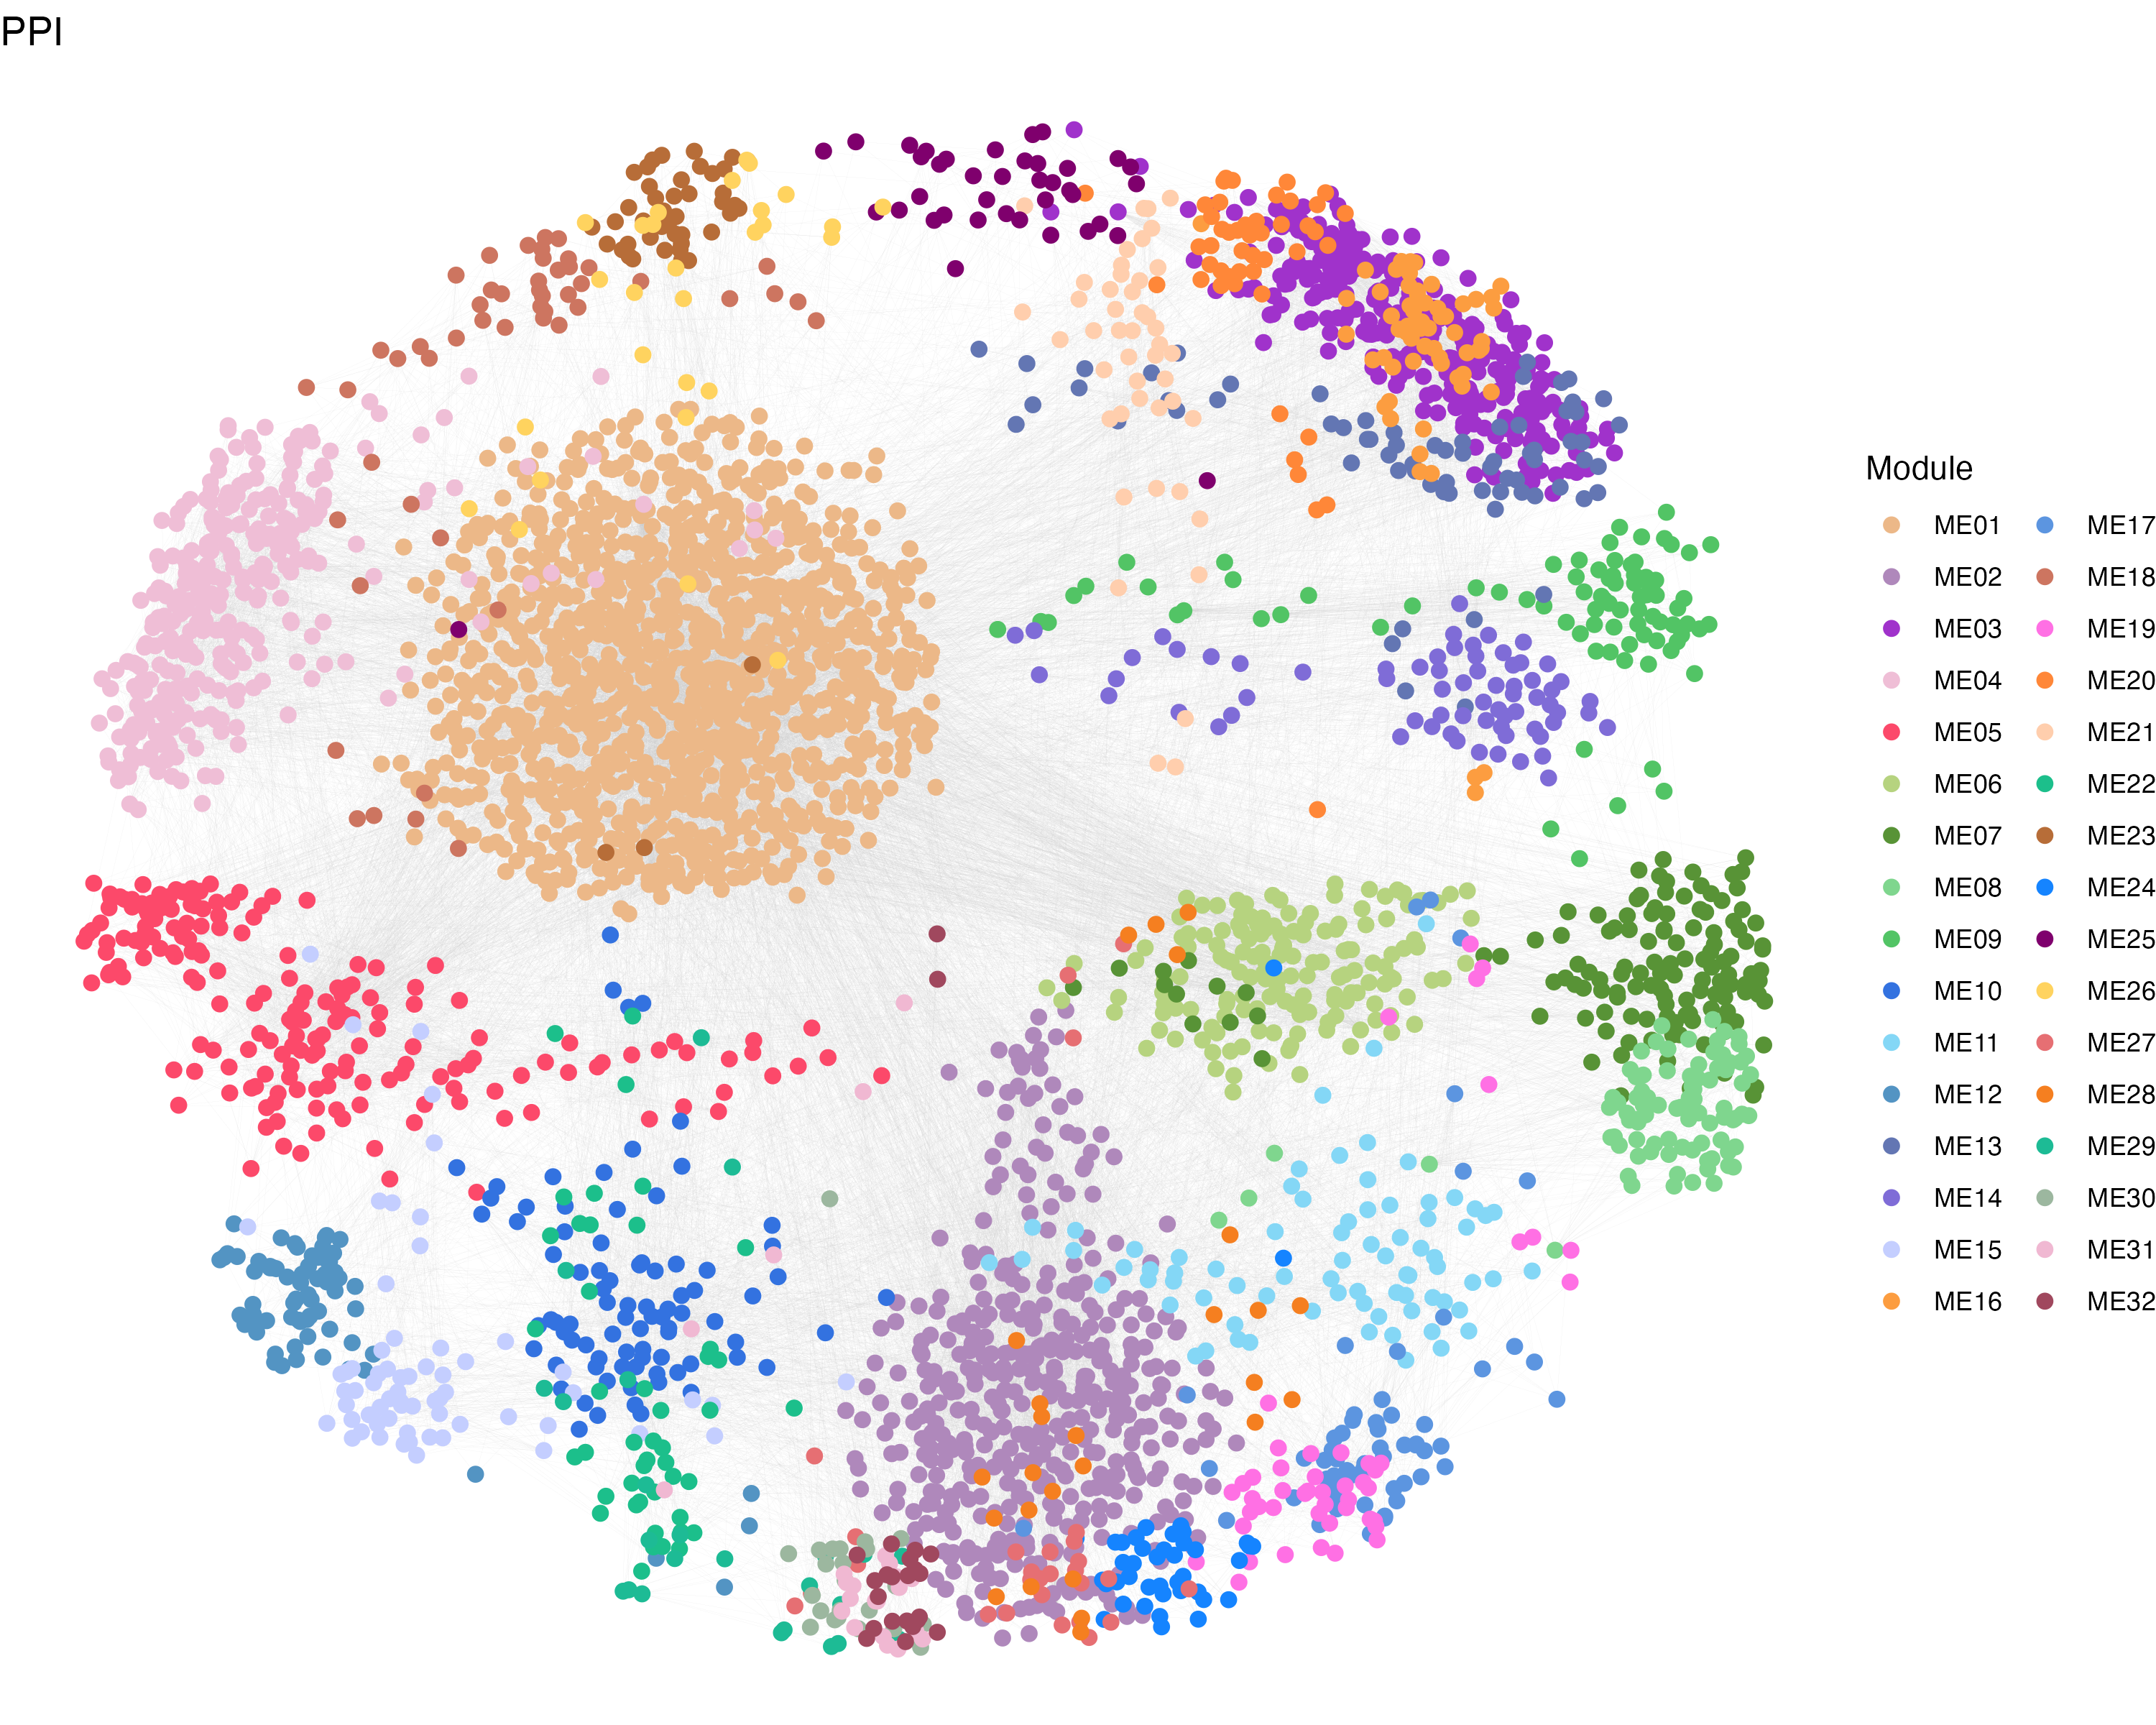
\includegraphics[width=0.9\linewidth]{Figures/2A-PRO-modules.png}
          \end{center}
        \end{figure}
    \end{column}

    \begin{column}{0.45\textwidth}
        \begin{figure}
          \begin{center}
            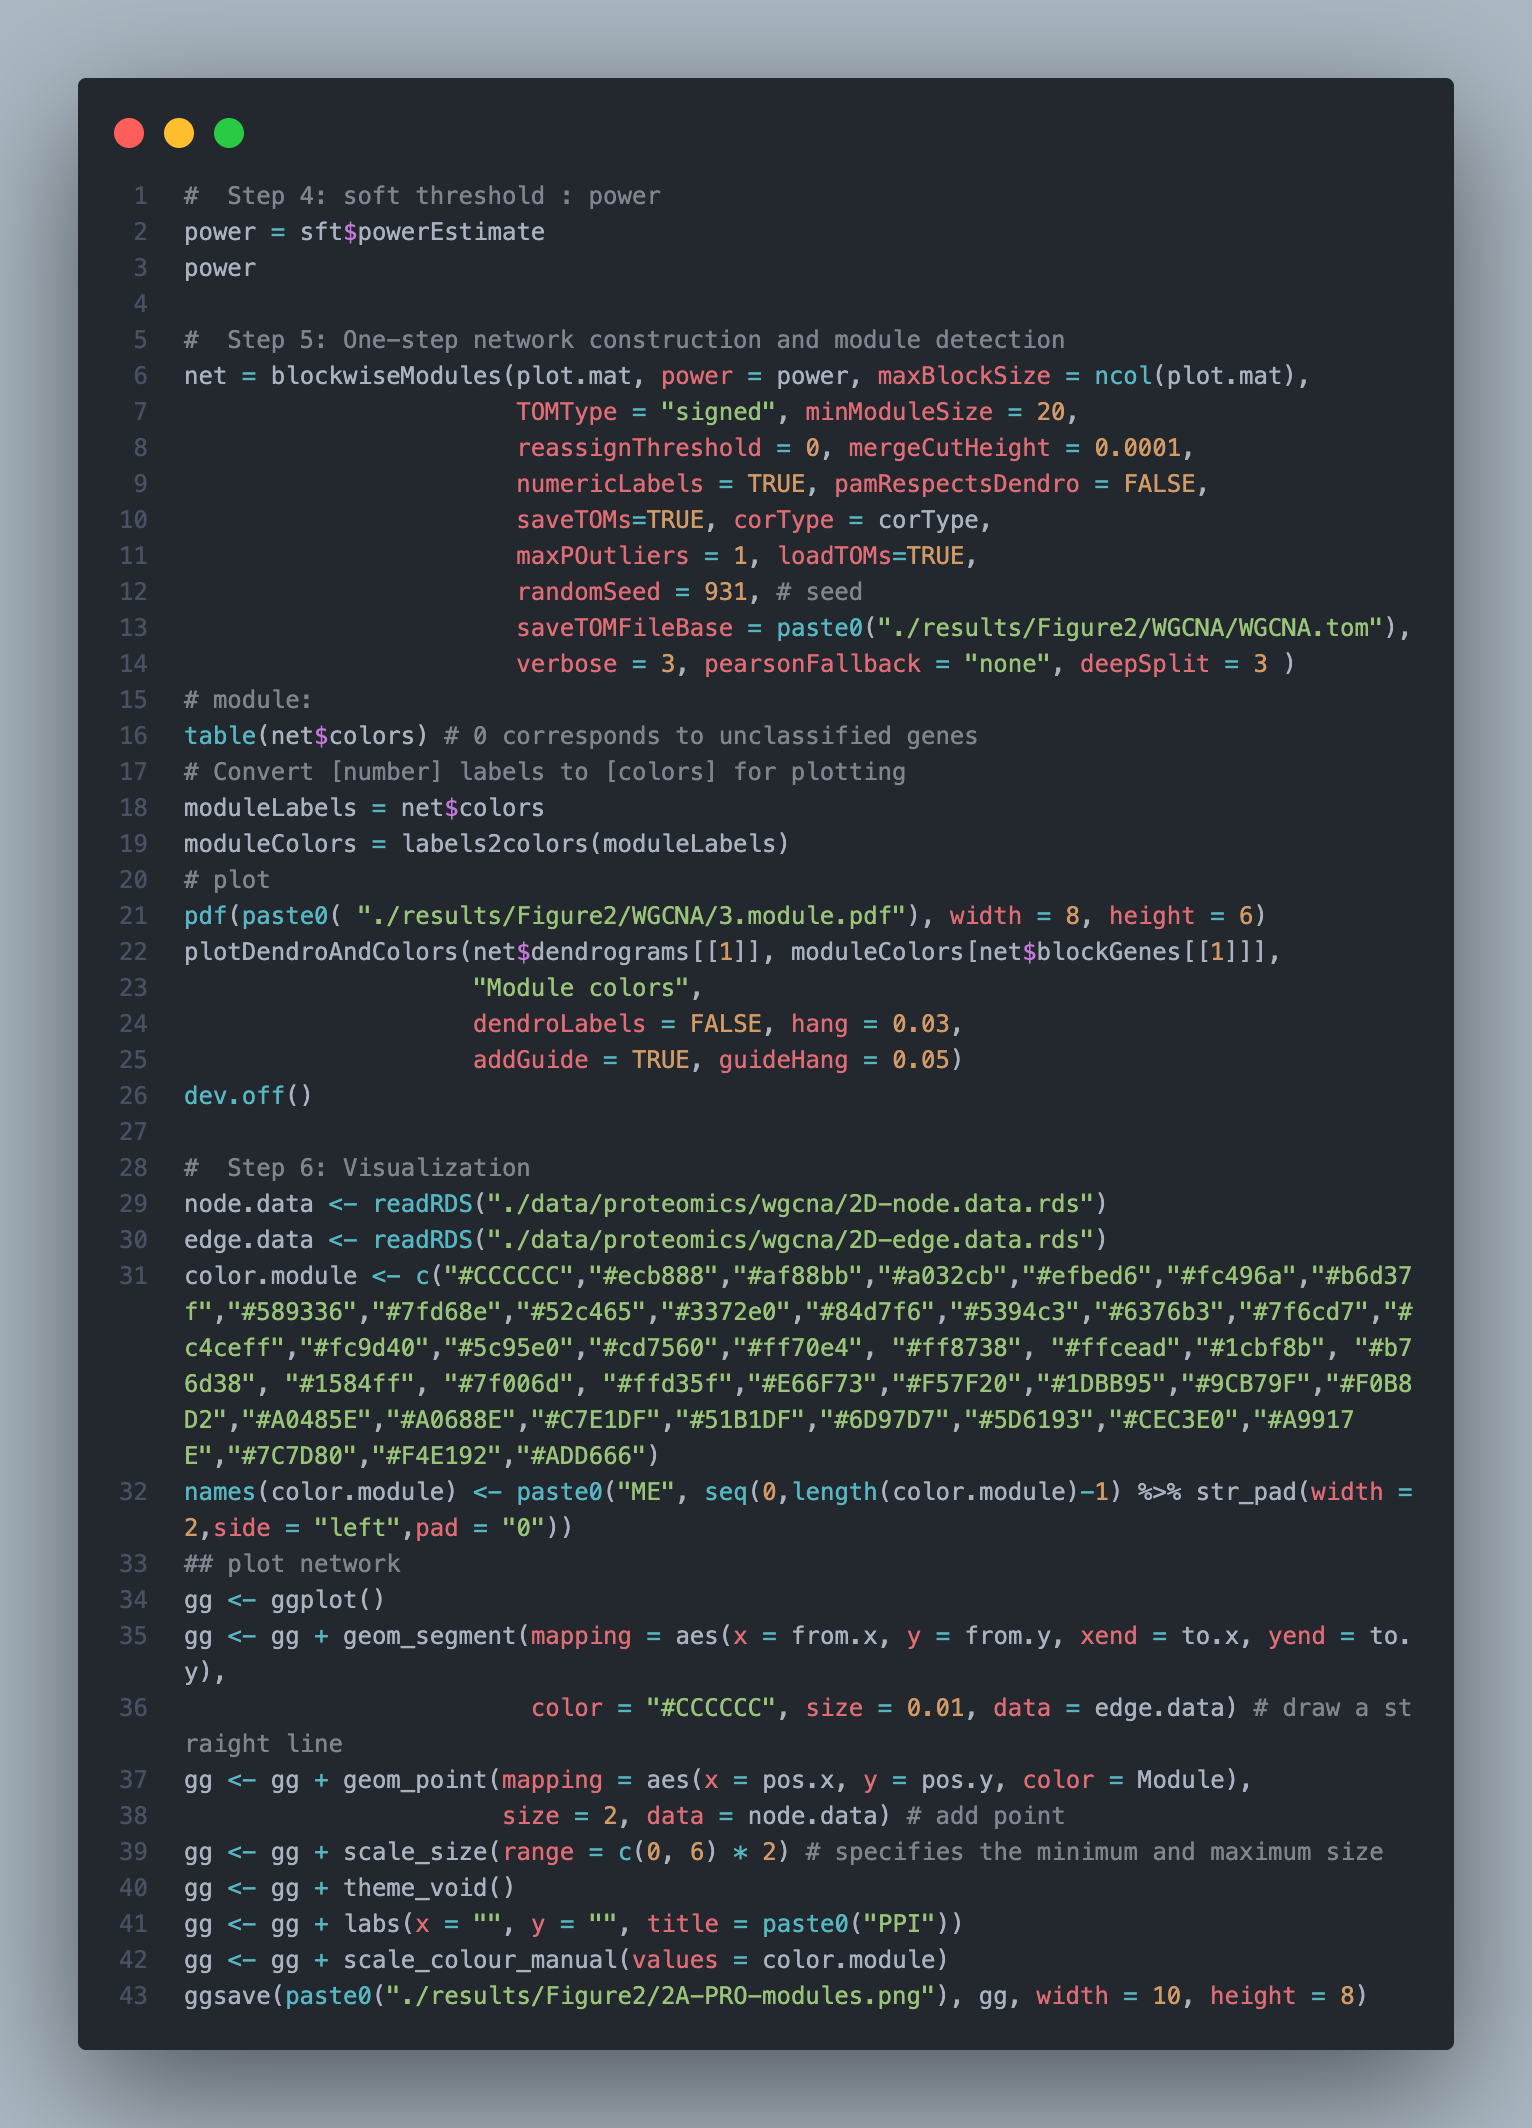
\includegraphics[width=0.9\linewidth]{Figures/2A-PRO-modules-code2.png}
          \end{center}
        \end{figure}
    \end{column}
  \end{columns}

  \vspace{0.5cm}
  We performed weighted correlation network analysis WGCNA on proteomic data from tumor samples, identifying a total of 32 functional modules. 
\end{frame}

\begin{frame}{Figure \& Code}
  \begin{columns}[onlytextwidth]
    \begin{column}{0.55\textwidth}
        \begin{figure}
          \begin{center}
            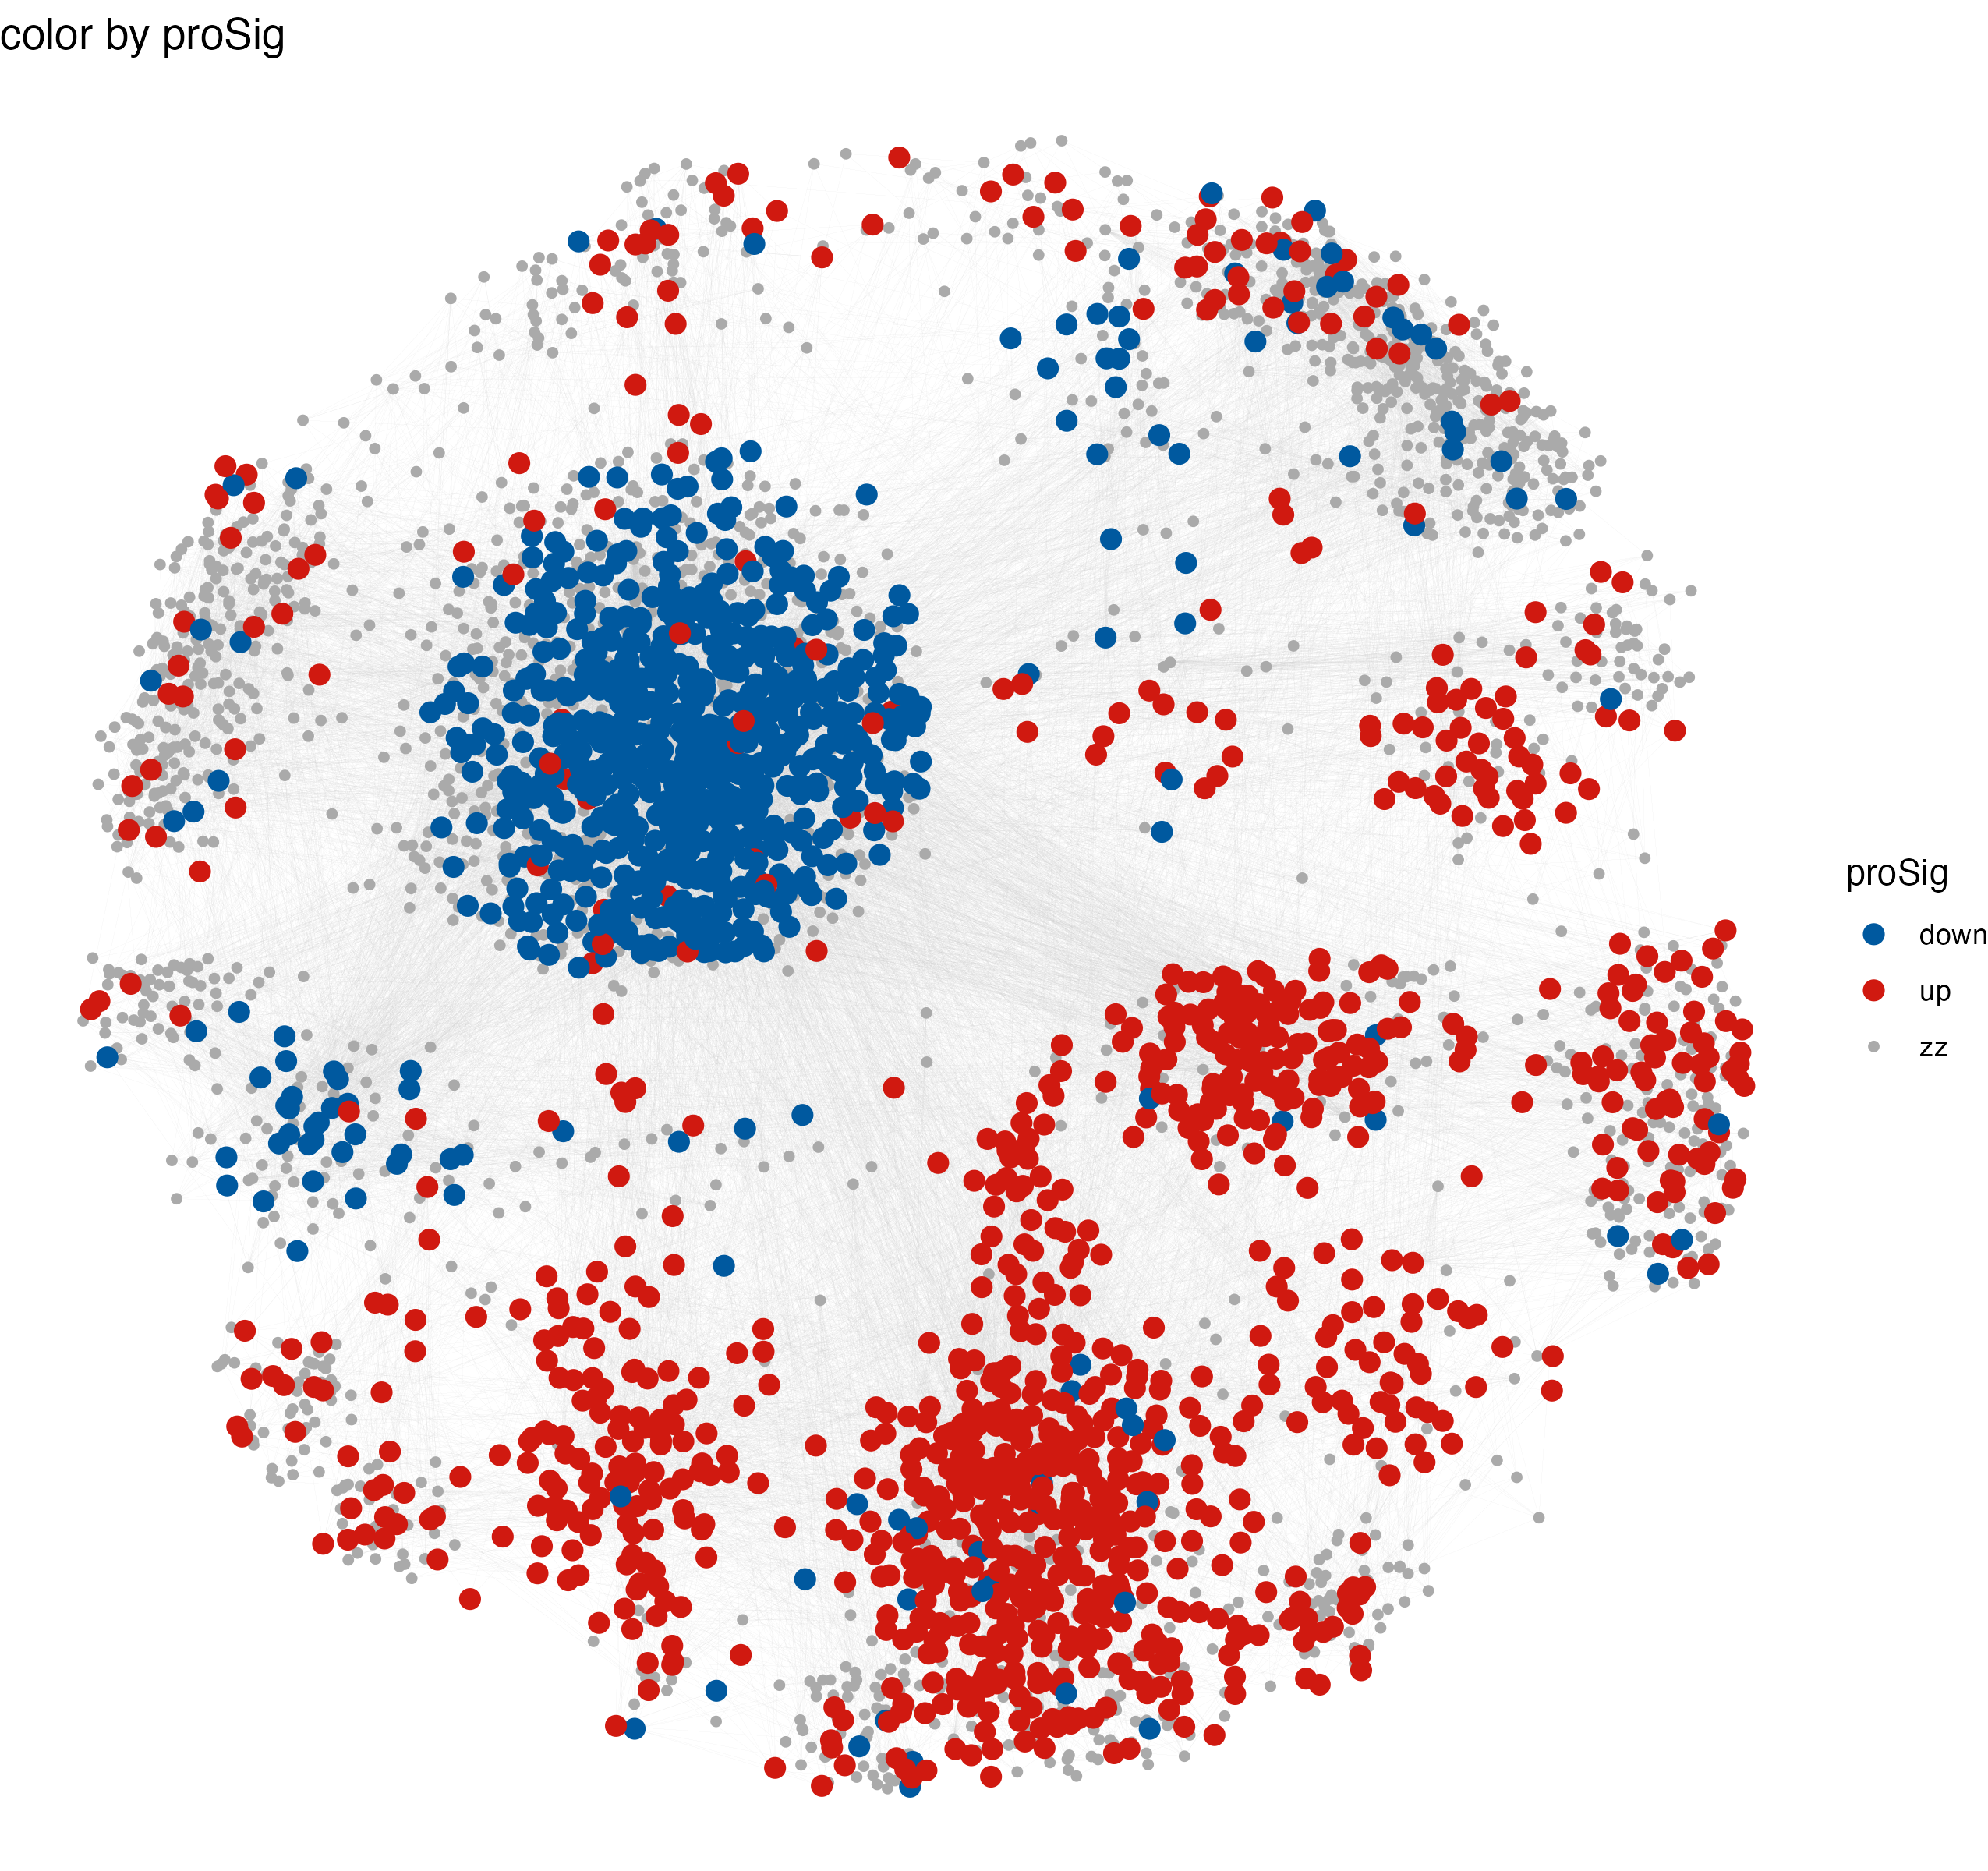
\includegraphics[width=0.9\linewidth]{Figures/2B-proSig.png}
          \end{center}
        \end{figure}
    \end{column}

    \begin{column}{0.45\textwidth}
        \begin{figure}
          \begin{center}
            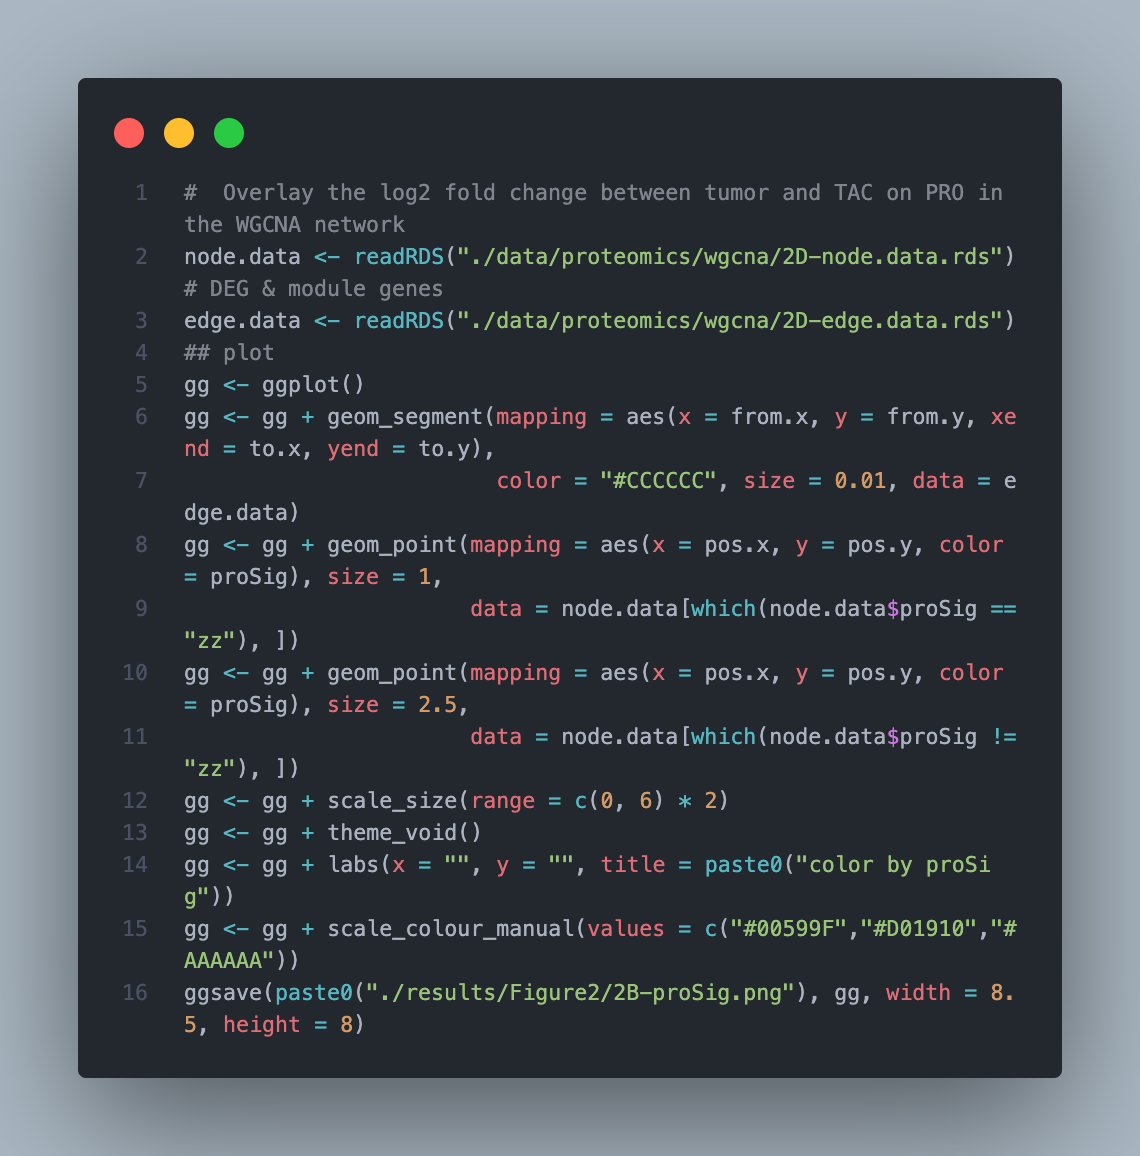
\includegraphics[width=0.9\linewidth]{Figures/2B-proSig-code.png}
          \end{center}
        \end{figure}
    \end{column}
  \end{columns}

  \vspace{0.5cm}
  Overlay of the significantly up/down-regulated proteins between tumors and TACs onto the network nodes. The proteins significantly up- or down-regulated within these modules, when comparing tumors and TACs are depicted this figure.
\end{frame}

\begin{frame}{Kaplan--Meier (KM) Survival Curve}
  \textbf{Goal:} non-parametric estimate of the survival function $S(t)=P(T>t)$.
  
  \begin{block}{Product-limit estimator}
    \[
    \widehat{S}(t)=\prod_{t_i\le t}\left(1-\frac{d_i}{n_i}\right)
    \]
    \begin{itemize}
        \item $t_i$: ordered event times
        \item $d_i$: events at $t_i$
        \item $n_i$: at risk just before $t_i$
    \end{itemize}
  \end{block}
  
  \begin{block}{How to read the plot}
    \begin{itemize}
      \item Step-down at each event; \textbf{ticks} mark censored samples
      \item \textbf{Median survival}: where $\widehat{S}(t)=0.5$
      \item Compare groups with \textbf{log-rank test}
    \end{itemize}
  \end{block}
\end{frame}

\begin{frame}{Figure \& Code}
  \begin{columns}[onlytextwidth]
    \begin{column}{0.3\textwidth}
        \begin{figure}
          \begin{center}
            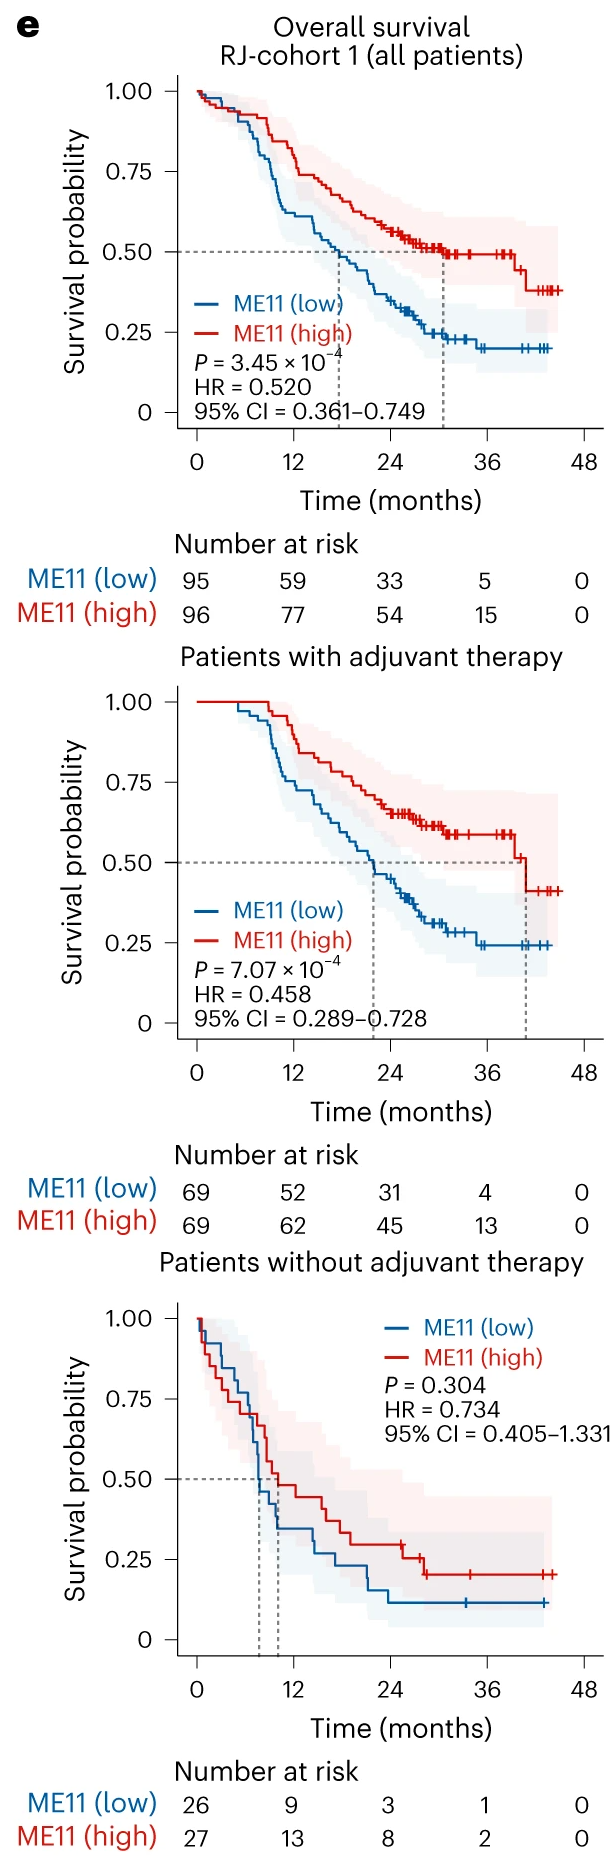
\includegraphics[width=0.7\linewidth]{Figures/Fig2e.png}
          \end{center}
        \end{figure}
    \end{column}

    \begin{column}{0.65\textwidth}
        \begin{figure}
          \begin{center}
            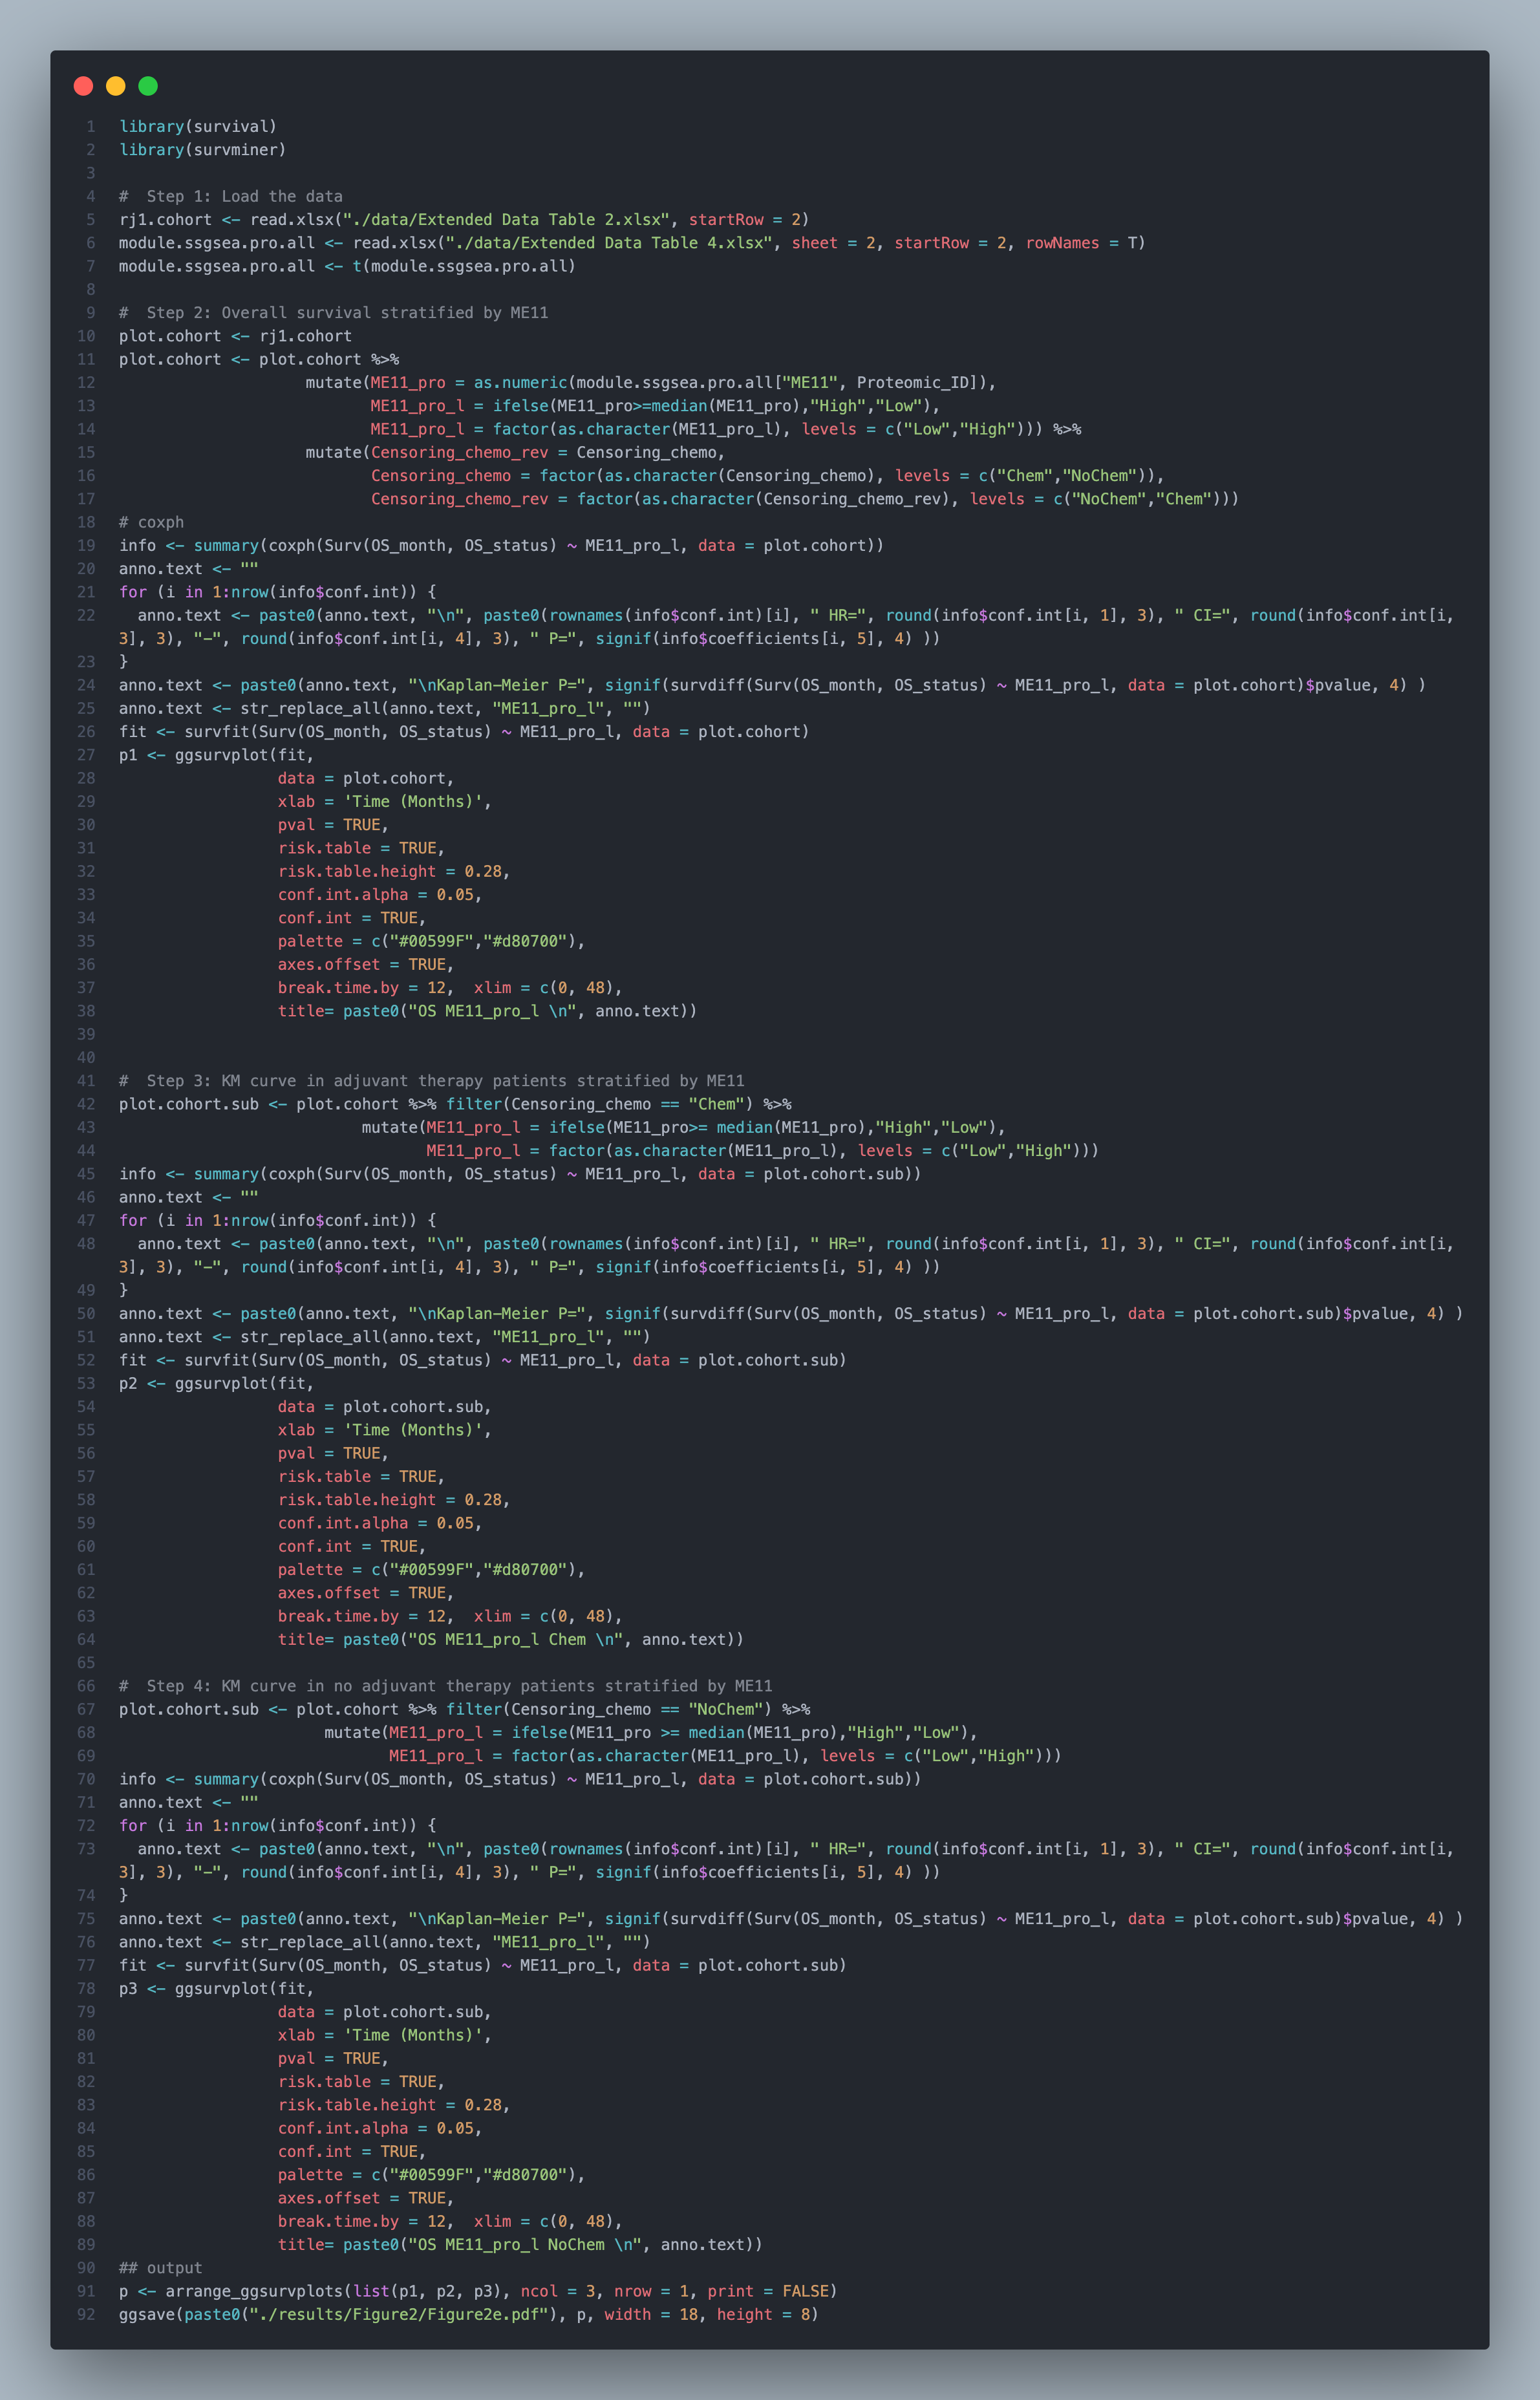
\includegraphics[width=0.7\linewidth]{Figures/Figure2e-code.png}
          \end{center}
        \end{figure}
    \end{column}
  \end{columns}
\end{frame}

\begin{frame}{Functional validation of selected protein modules}
  \vspace{0.3cm}

  \begin{columns}[onlytextwidth]
    \begin{column}{0.6\textwidth}
      \begin{itemize}
        \item Kaplan-Meier curves comparing OS between patient subgroups stratified by both adjuvant therapy and the high/low abundance (median cutoff) of ME11. 
        \item When receiving chemotherapy, individuals with higher ME11 show a clear upward shift in the survival curve, suggesting that high ME11 may enhance the benefit of postoperative adjuvant therapy.
        \item Without chemotherapy, the survival curves of the two ME11 expression groups show no obvious difference, which may indicate a specific role of the ME11 module in chemotherapy sensitivity.
      \end{itemize}
    \end{column}

    \begin{column}{0.4\textwidth}
        \begin{figure}
          \begin{center}
            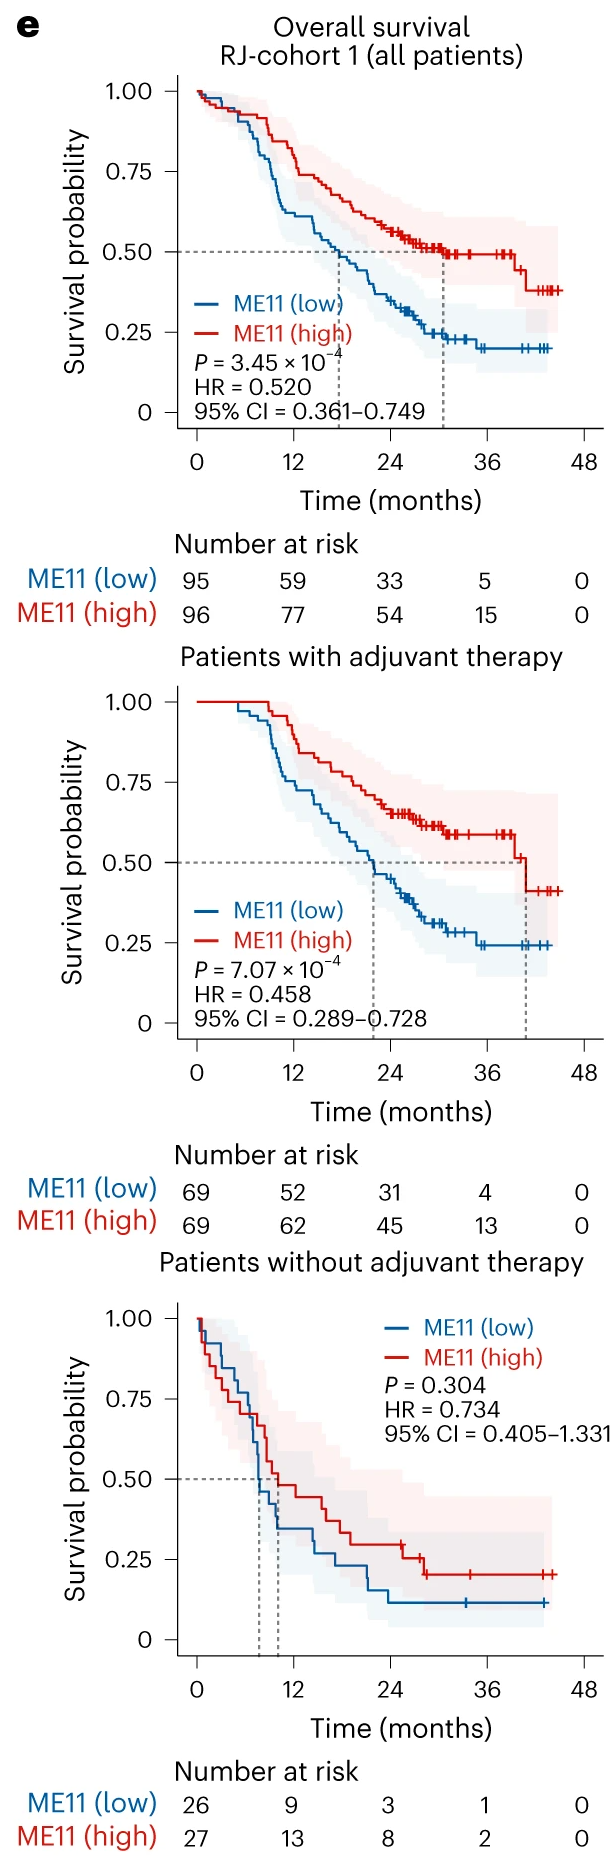
\includegraphics[width=0.5\linewidth]{Figures/Fig2e.png}
          \end{center}
          \caption{ME11 KM plot}
        \end{figure}
    \end{column}

  \end{columns}
\end{frame}



\begin{frame}{Refined selection: LASSO-Cox regression}

  \begin{block}{1. Cox proportional hazards model}
    This is a core model in survival analysis to study how one or more covariates affect the hazard of an event (e.g., death or recurrence).
    \vspace{0.3em}
    \[
      h(t\mid X)=h_0(t)\,\exp(\beta_1X_1+\beta_2X_2+\cdots+\beta_{p}X_{p})
    \]
    \begin{itemize}
      \item $h(t\mid X)$: hazard at time $t$ given covariates $X$.
      \item $h_0(t)$: baseline hazard function (time-varying, shared across individuals).
      \item $\exp(\beta_1X_1+\cdots)$: risk ratio component with coefficients $\beta$.
    \end{itemize}
    \textbf{Features:} The Cox model is a semi-parametric model. It does not assume a specific functional form for $h_0(t)$ and estimates the coefficients $\beta$ using partial likelihood. The coefficients $\beta$ are interpreted as follows: holding other variables constant, for each one-unit increase in $X_j$, the log hazard ratio changes by $\beta_j$. Thus, $\exp(\beta_j)$ is the hazard ratio.
  \end{block}

\end{frame}

\begin{frame}{Refined selection: LASSO-Cox regression}
  \begin{block}{2. LASSO (Least Absolute Shrinkage and Selection Operator)}
    A regularization method for feature selection and reducing overfitting by adding an L1 penalty:
    \[
      \lambda\sum_j\lvert\beta_j\rvert,\quad \lambda>0.
    \]
    \begin{itemize}
      \item Shrinks unimportant coefficients toward 0 (automatic feature selection).
      \item Handles collinearity by preferring a simpler subset of variables.
      \item Improves generalization by reducing model complexity.
    \end{itemize}
  \end{block}
\end{frame}

\begin{frame}{LASSO selection}
   Using LASSO-Cox regression, we can select key high-scoring proteins from many protein modules for further study.

  \vspace{0.6em}

  \begin{figure}
    \begin{center}
      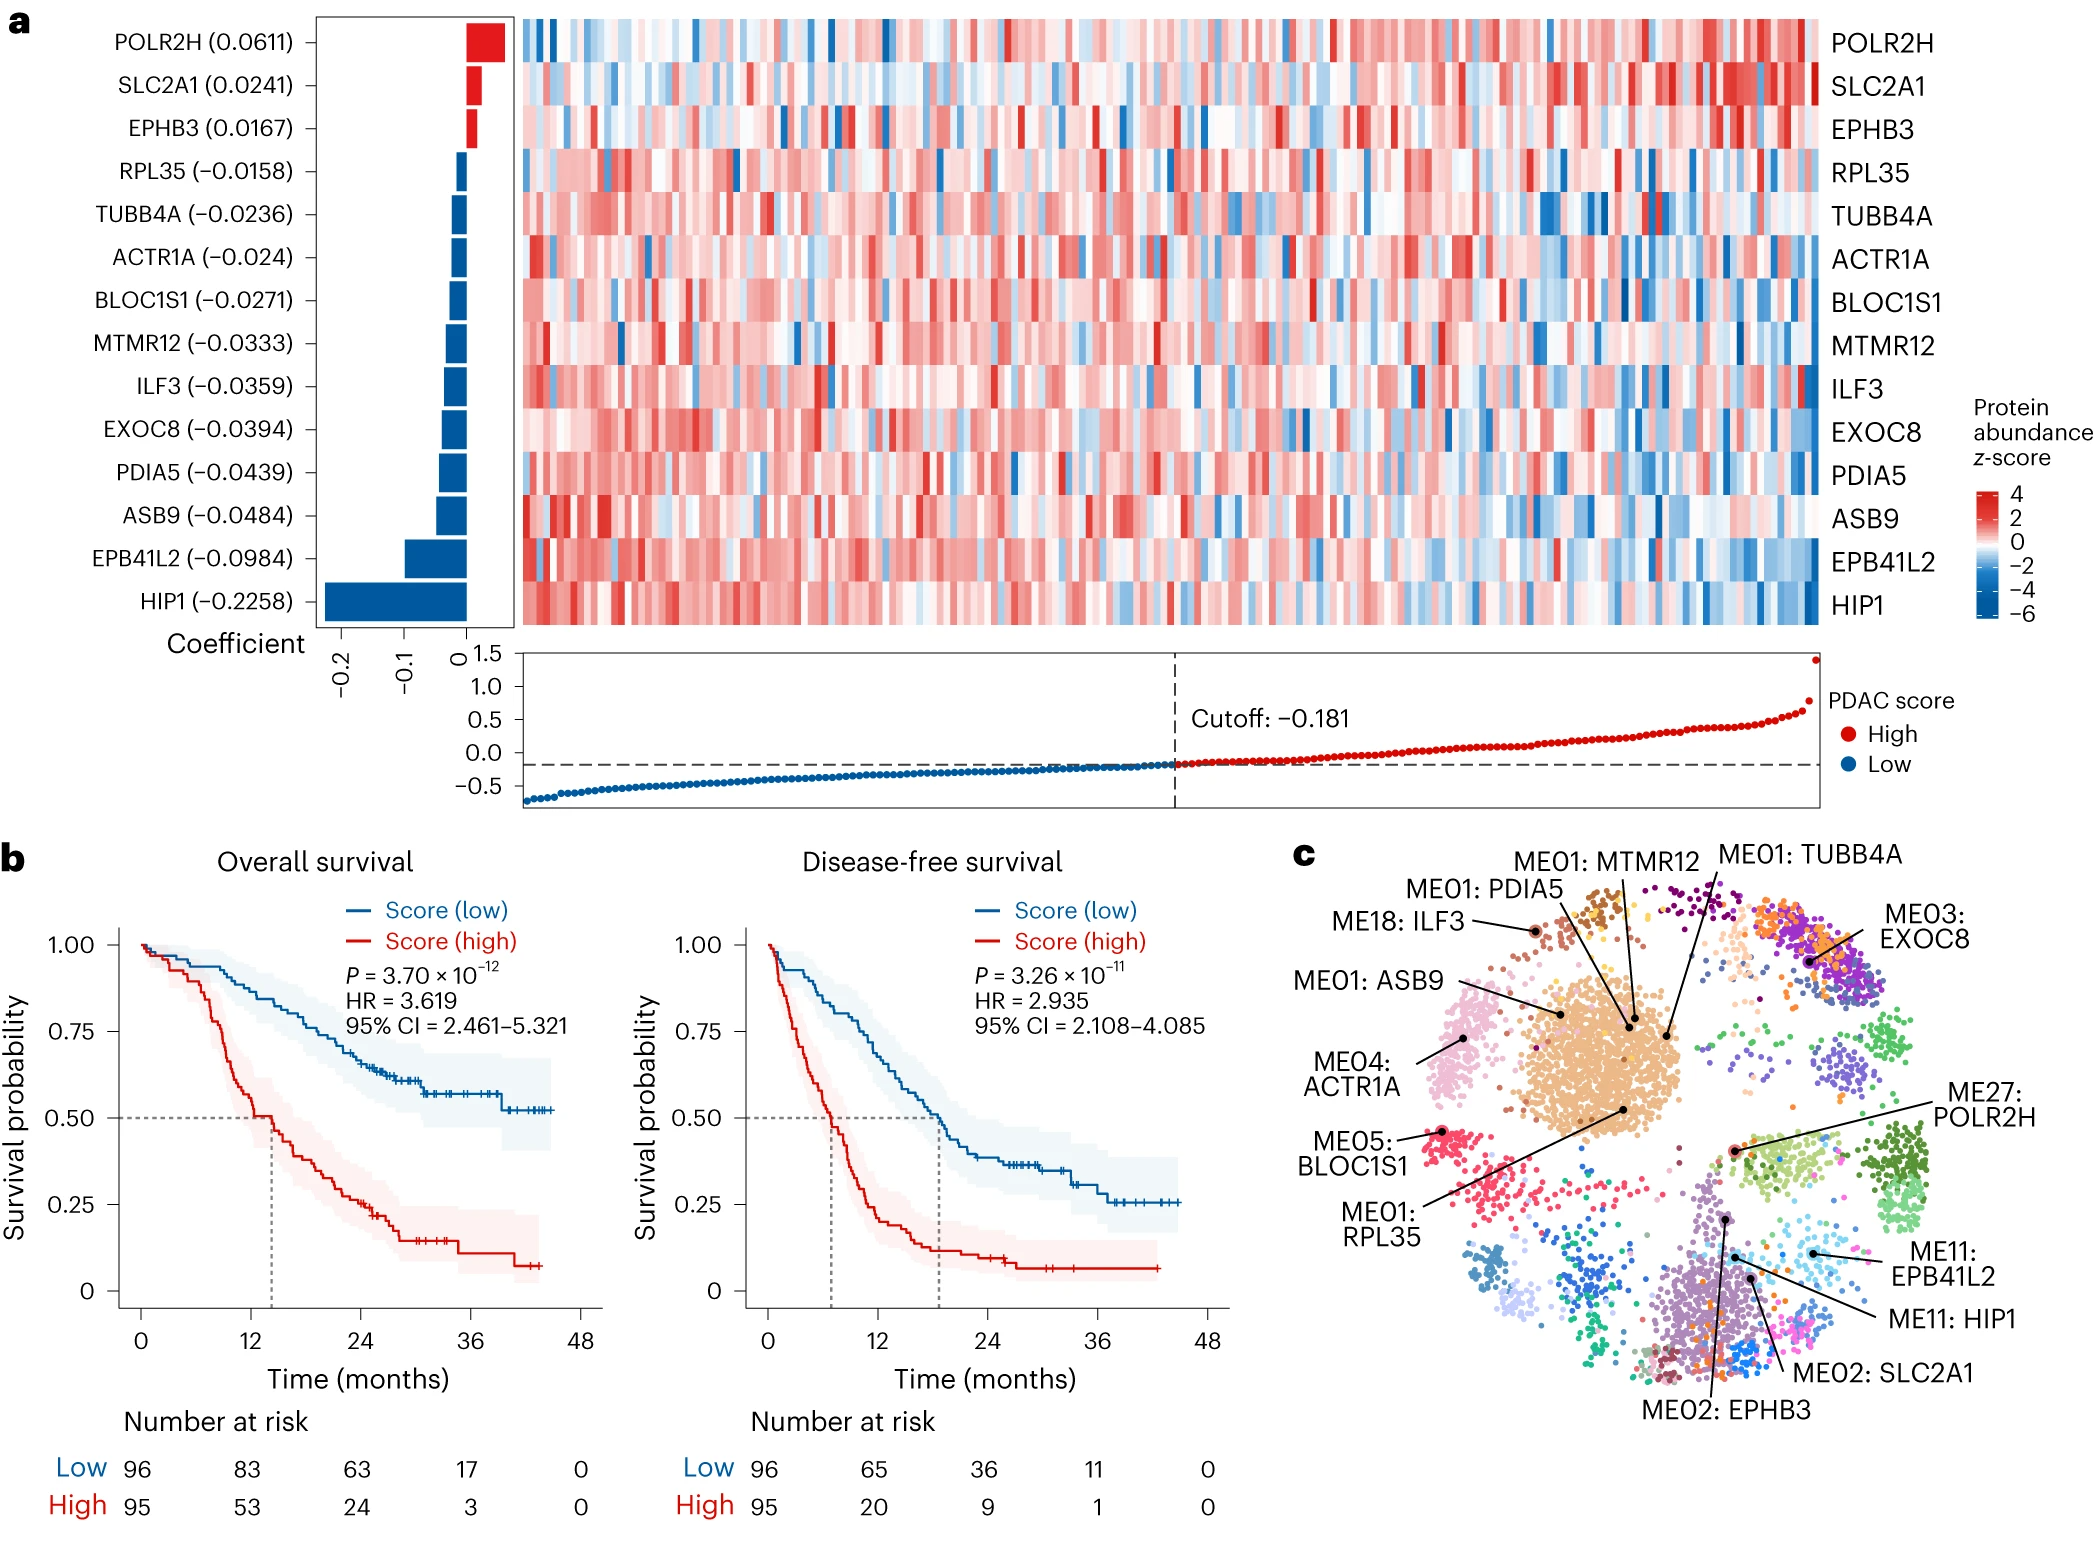
\includegraphics[width=0.7\linewidth]{Figures/Fig3a-c.png}
    \end{center}
    \caption{LASSO selection}
  \end{figure}
\end{frame}

\begin{frame}{Figure \& Code}
  \begin{figure}
    \begin{center}
      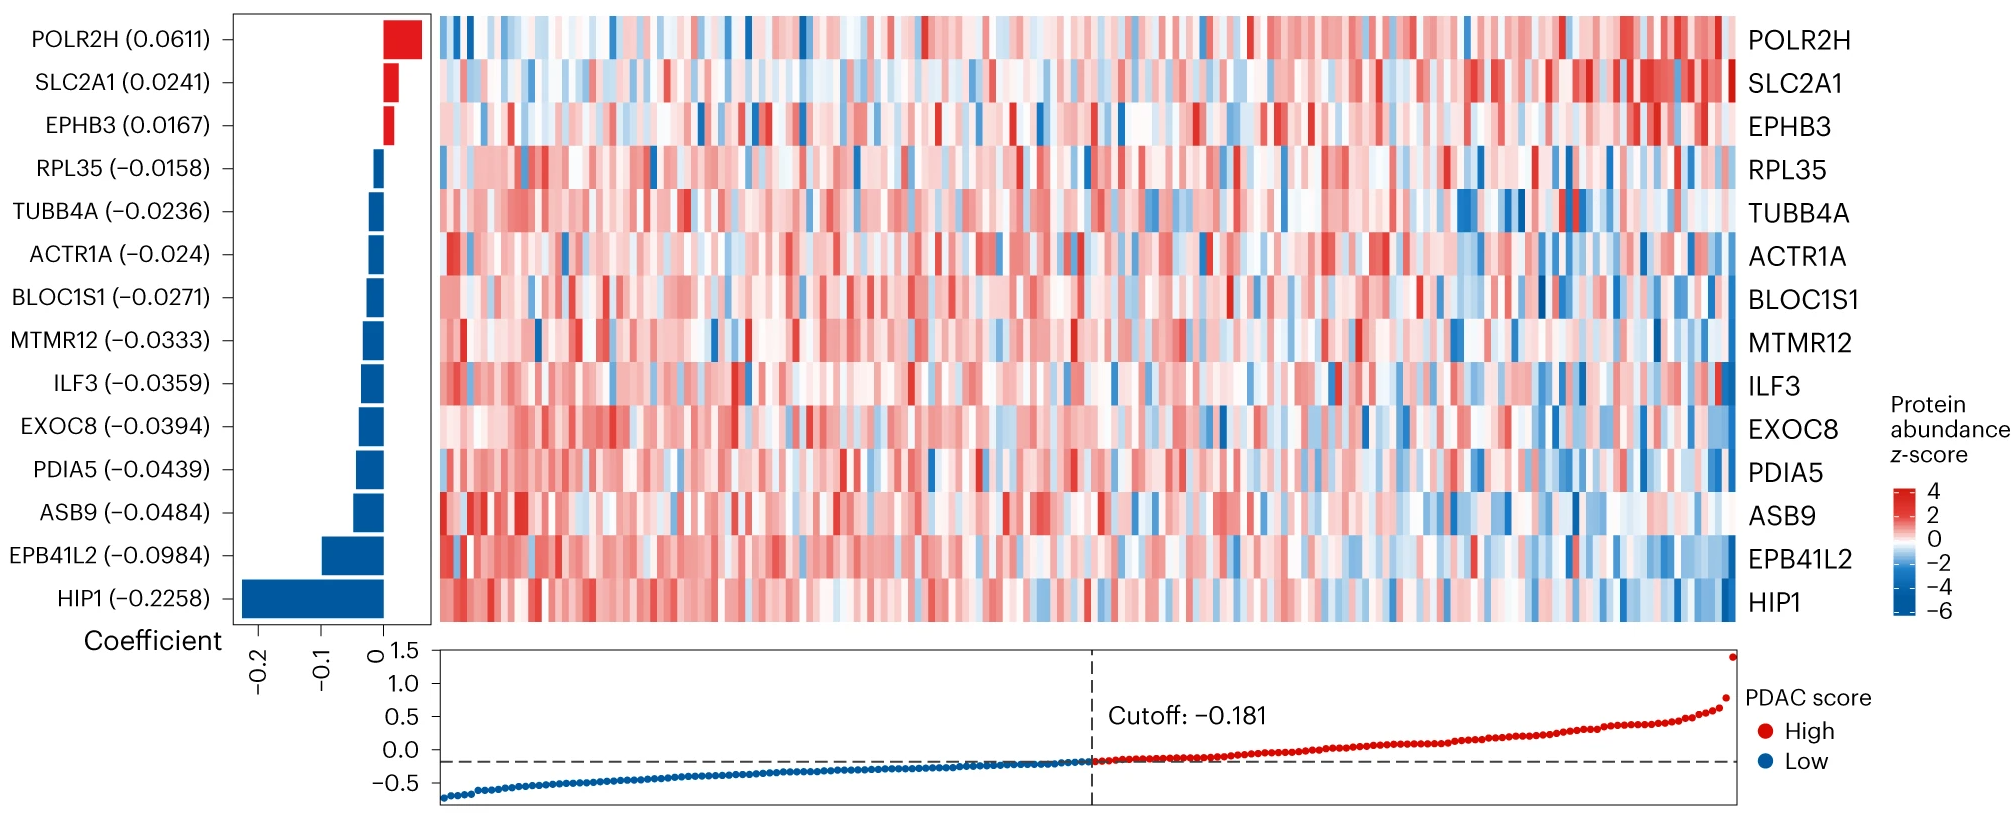
\includegraphics[width=0.7\linewidth]{Figures/Fig3a.png}
    \end{center}
  \end{figure}
  \vspace{0.5cm}
  LASSO model for PDAC. The left panel shows the regression coefficients of 14 proteins in the LASSO–Cox regression model. The right heat map displays the protein abundance of these 14 proteins in each patient with PDAC. The bottom scatter plot presents the LASSO score across patients with PDAC, with patients ordered according to their LASSO score and stratified into two groups based on the median value of the score
\end{frame}

\begin{frame}{Figure \& Code}
  \begin{columns}[onlytextwidth]
    \begin{column}{0.47\textwidth}
        \begin{figure}
          \begin{center}
            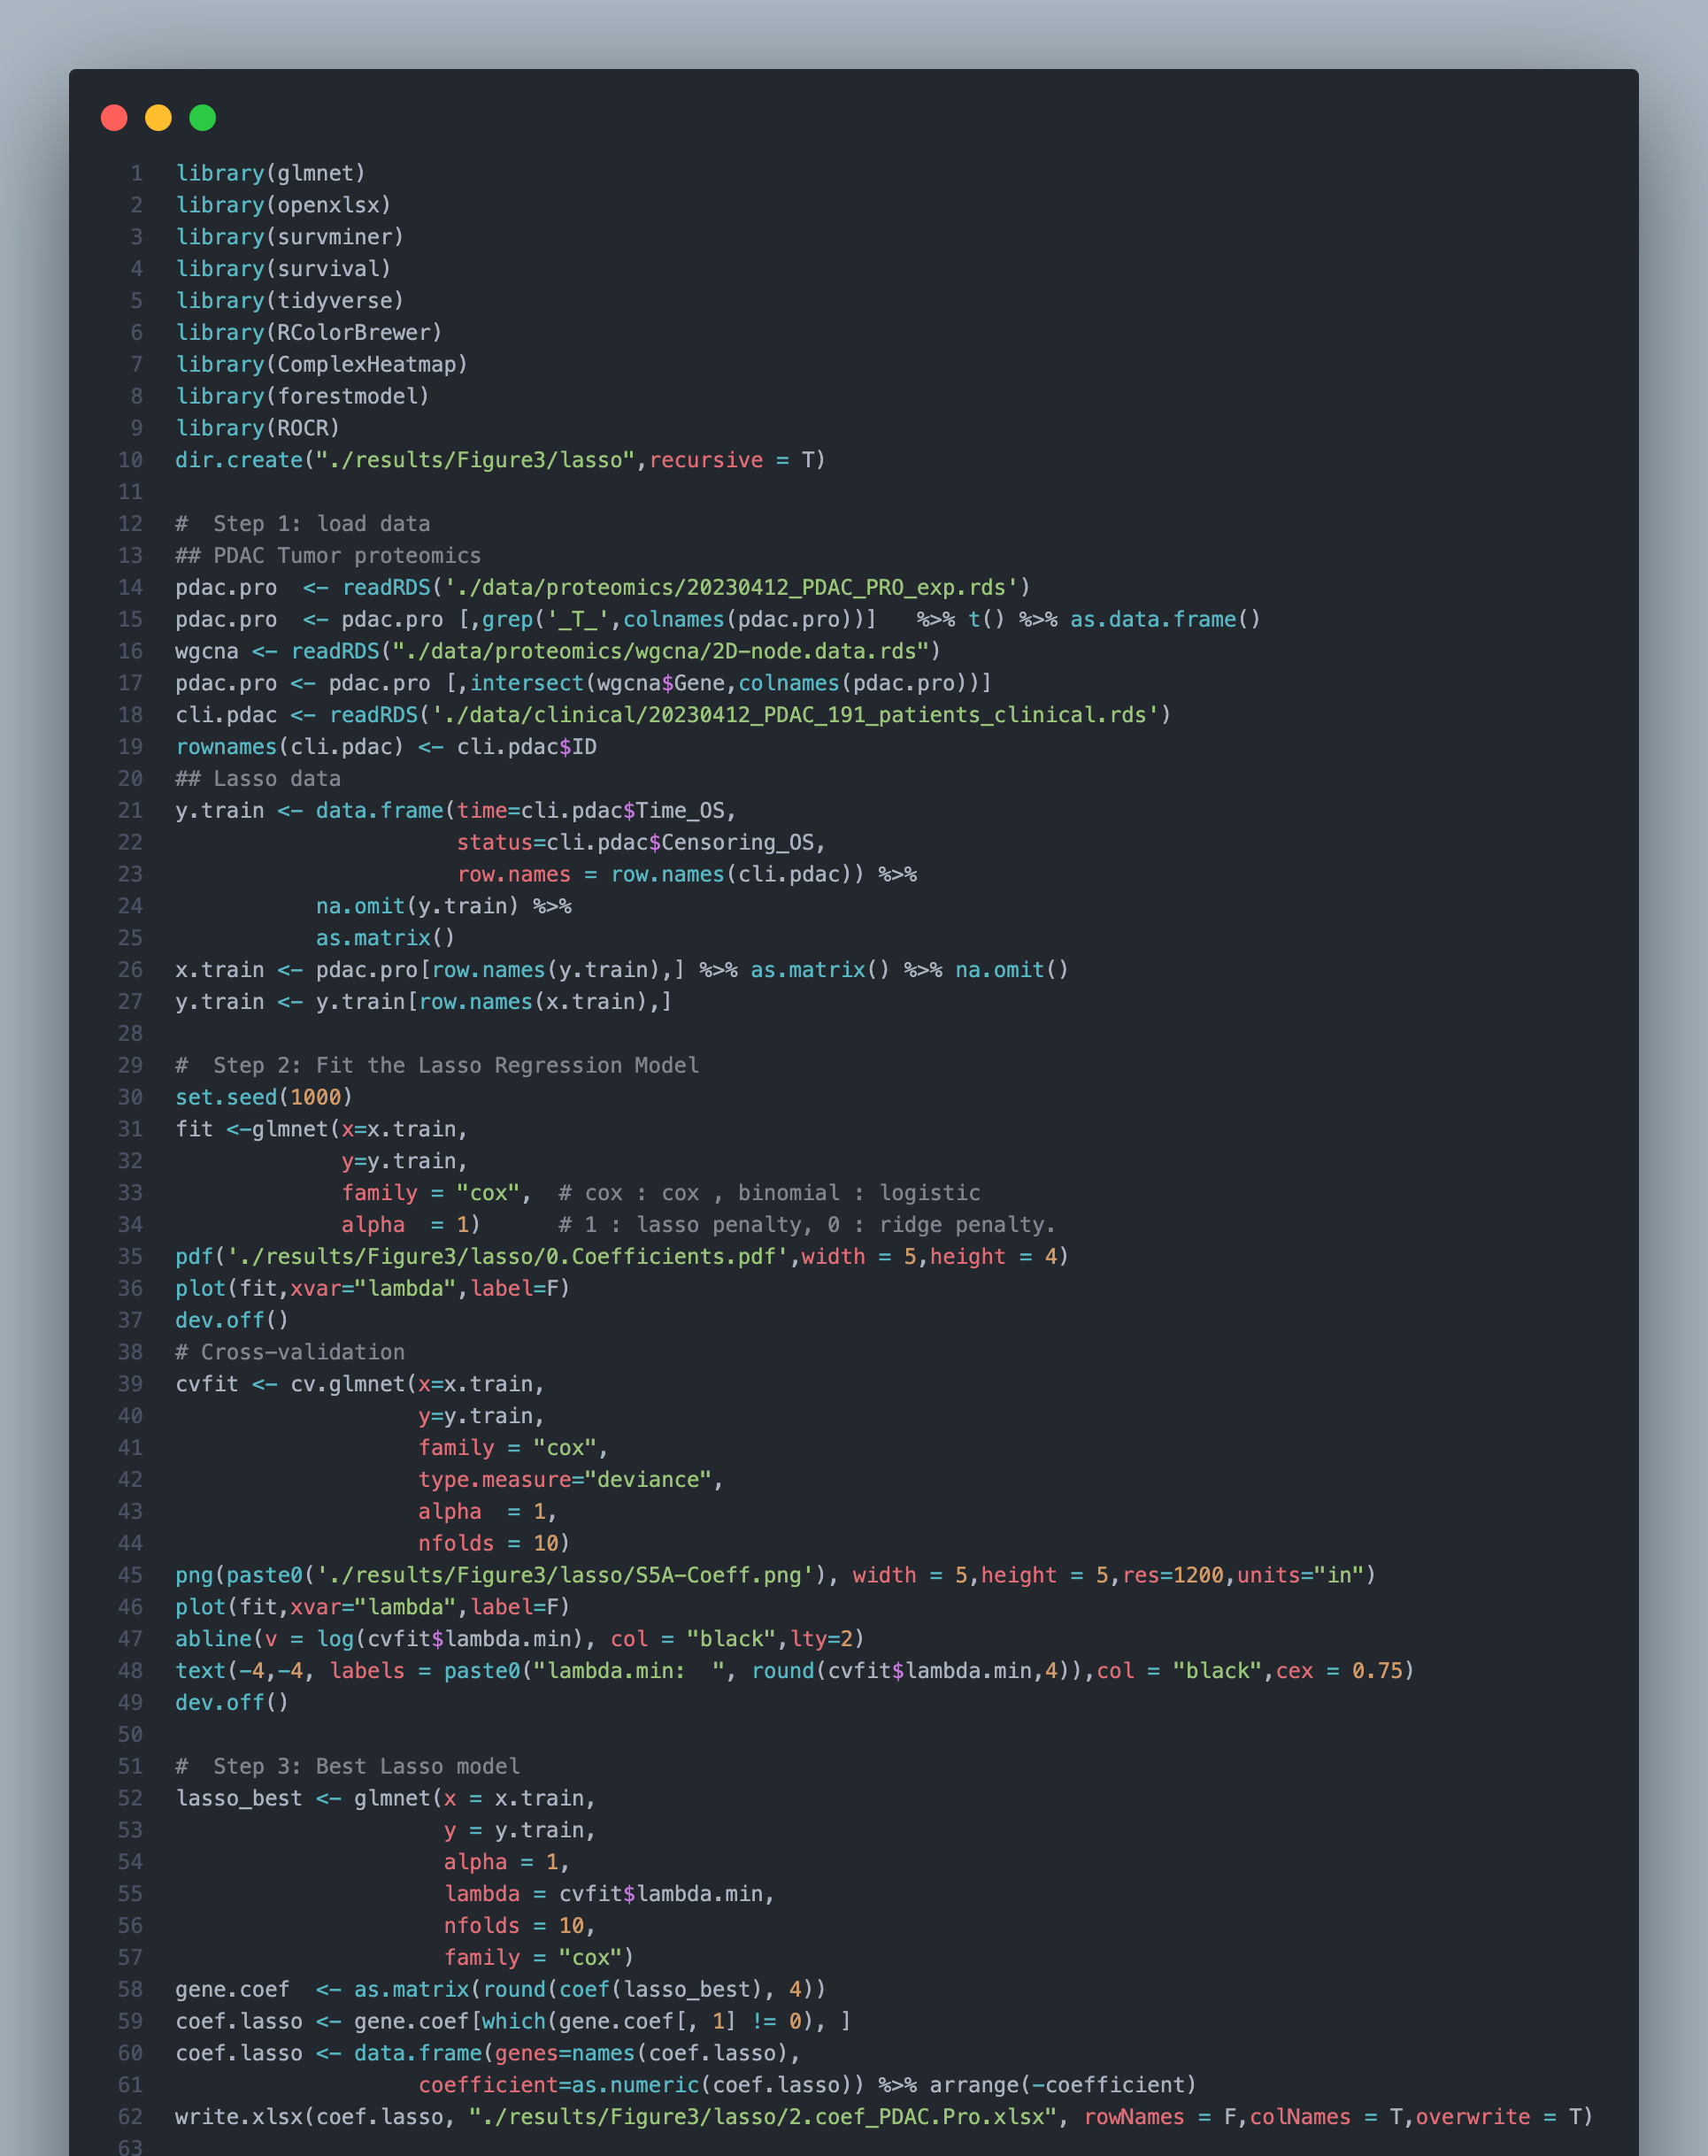
\includegraphics[width=\linewidth]{Figures/Fig3a-code1.png}
          \end{center}
        \end{figure}
    \end{column}

    \begin{column}{0.47\textwidth}
        \begin{figure}
          \begin{center}
            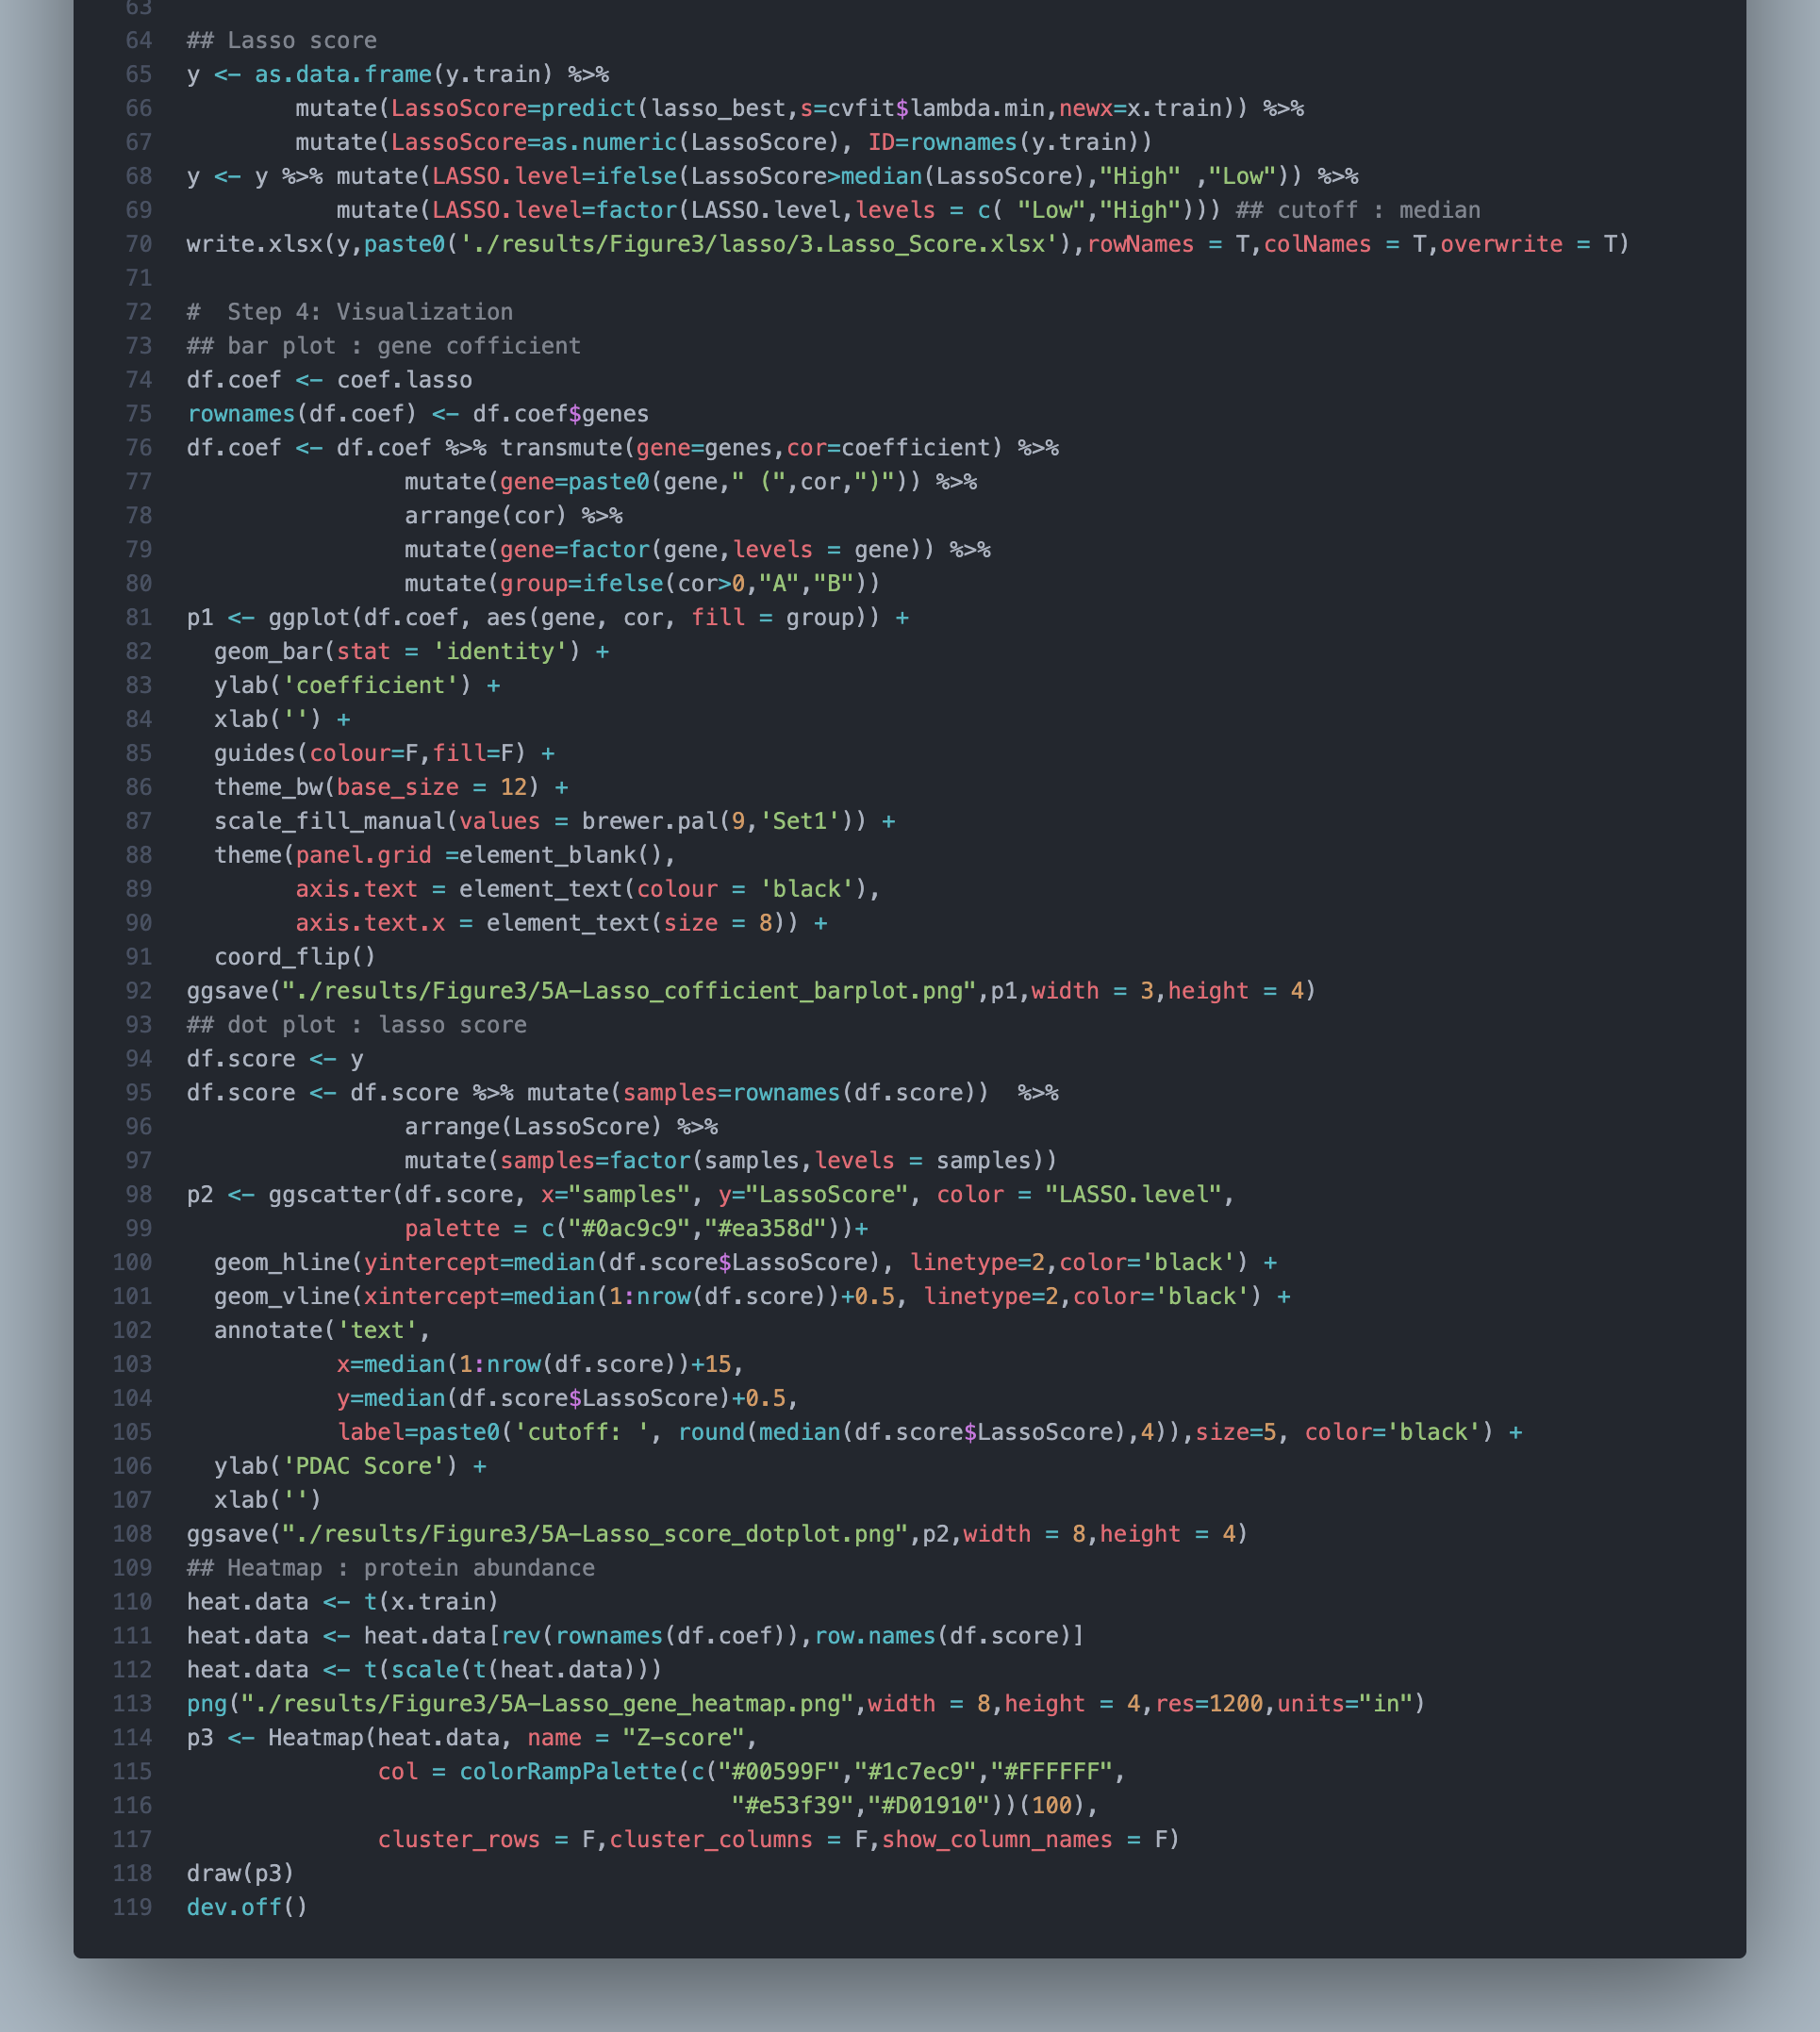
\includegraphics[width=\linewidth]{Figures/Fig3a-code2.png}
          \end{center}
        \end{figure}
    \end{column}
  \end{columns}
\end{frame}

\begin{frame}{Important factor: Chemotherapy sensitivity}
  \begin{itemize}
    \item In the previous analysis, we did not introduce the condition of ``chemotherapy sensitivity''; we only selected proteins that affect survival after postoperative adjuvant therapy.
    \item We want to find proteins whose expression level shows a very strong association with survival only when combined with the condition of ``receiving chemotherapy''.
  \end{itemize}

  \vspace{0.4em}

  \begin{center}
  \emph{``More specifically, we employed Cox proportional hazards models that incorporated the chemotherapy-by-biomarker interaction term for OS.''}
  \end{center}
\end{frame}

\begin{frame}{Cox regression analysis incorporating chemotherapy}
  \begin{figure}
    \begin{center}
      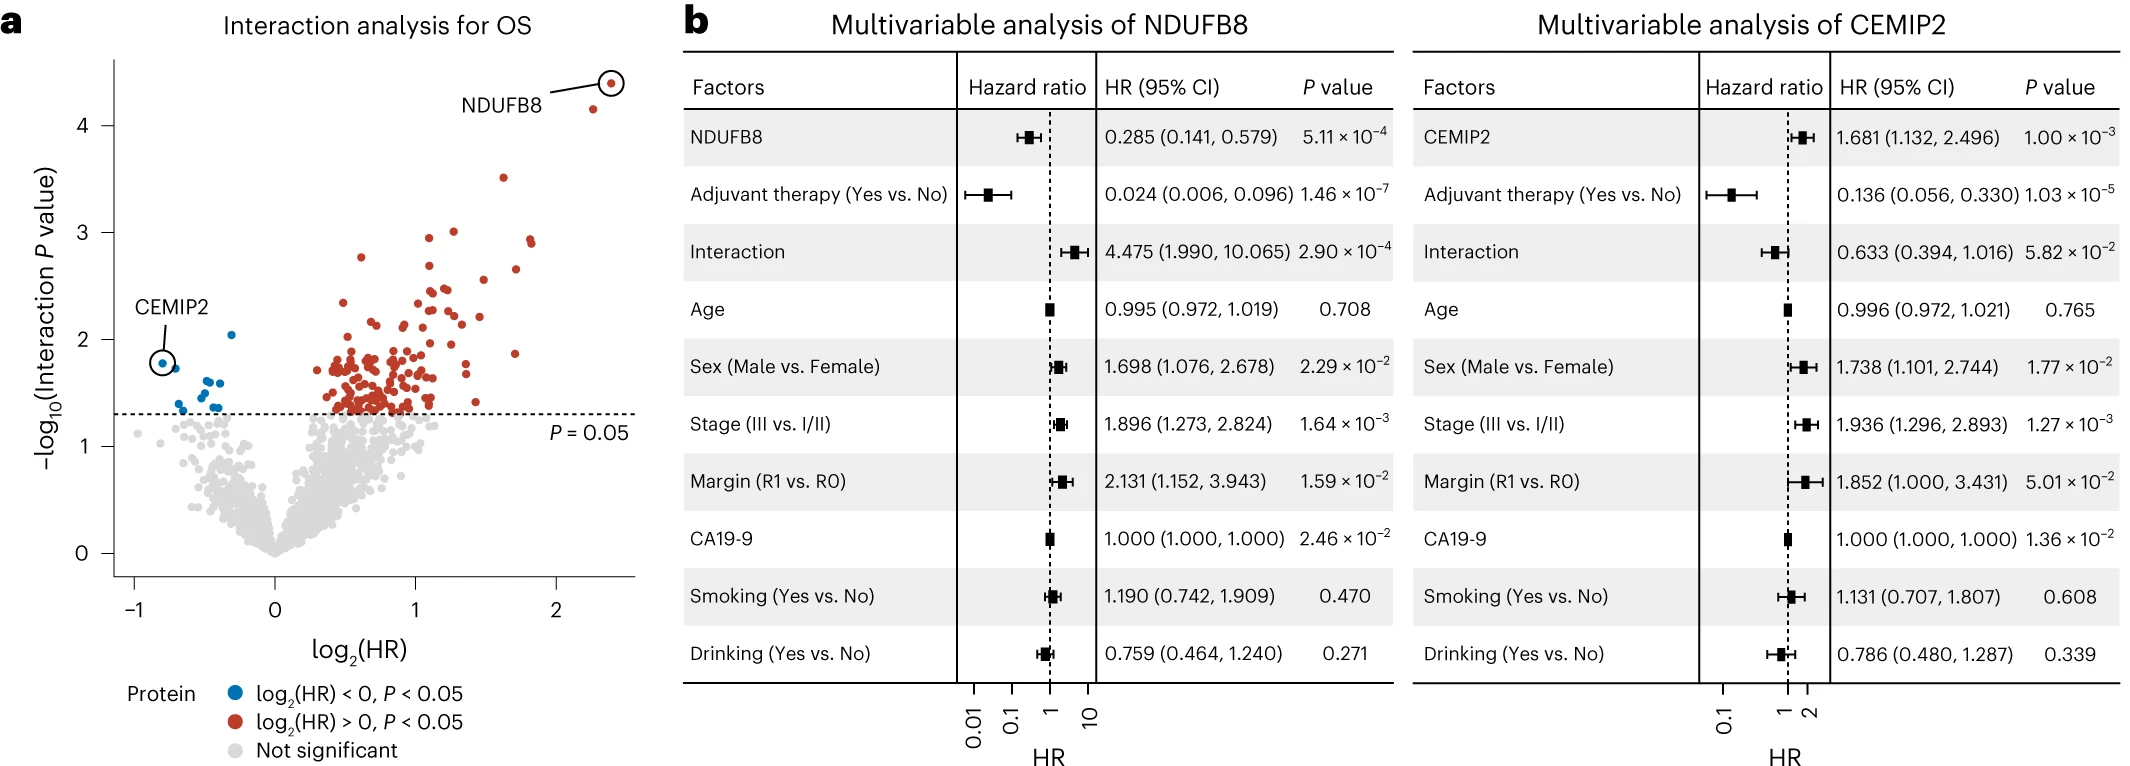
\includegraphics[width=\linewidth]{Figures/Fig4ab.png}
    \end{center}
    \caption{Cox regression analysis incorporating chemotherapy}
  \end{figure}

  \centering \textbf{Two biomarkers: CEMIP and NDUFB8}
\end{frame}

\begin{frame}{Figure \& Code}
  \begin{columns}[onlytextwidth]
    \begin{column}{0.6\textwidth}
        \begin{figure}
          \begin{center}
            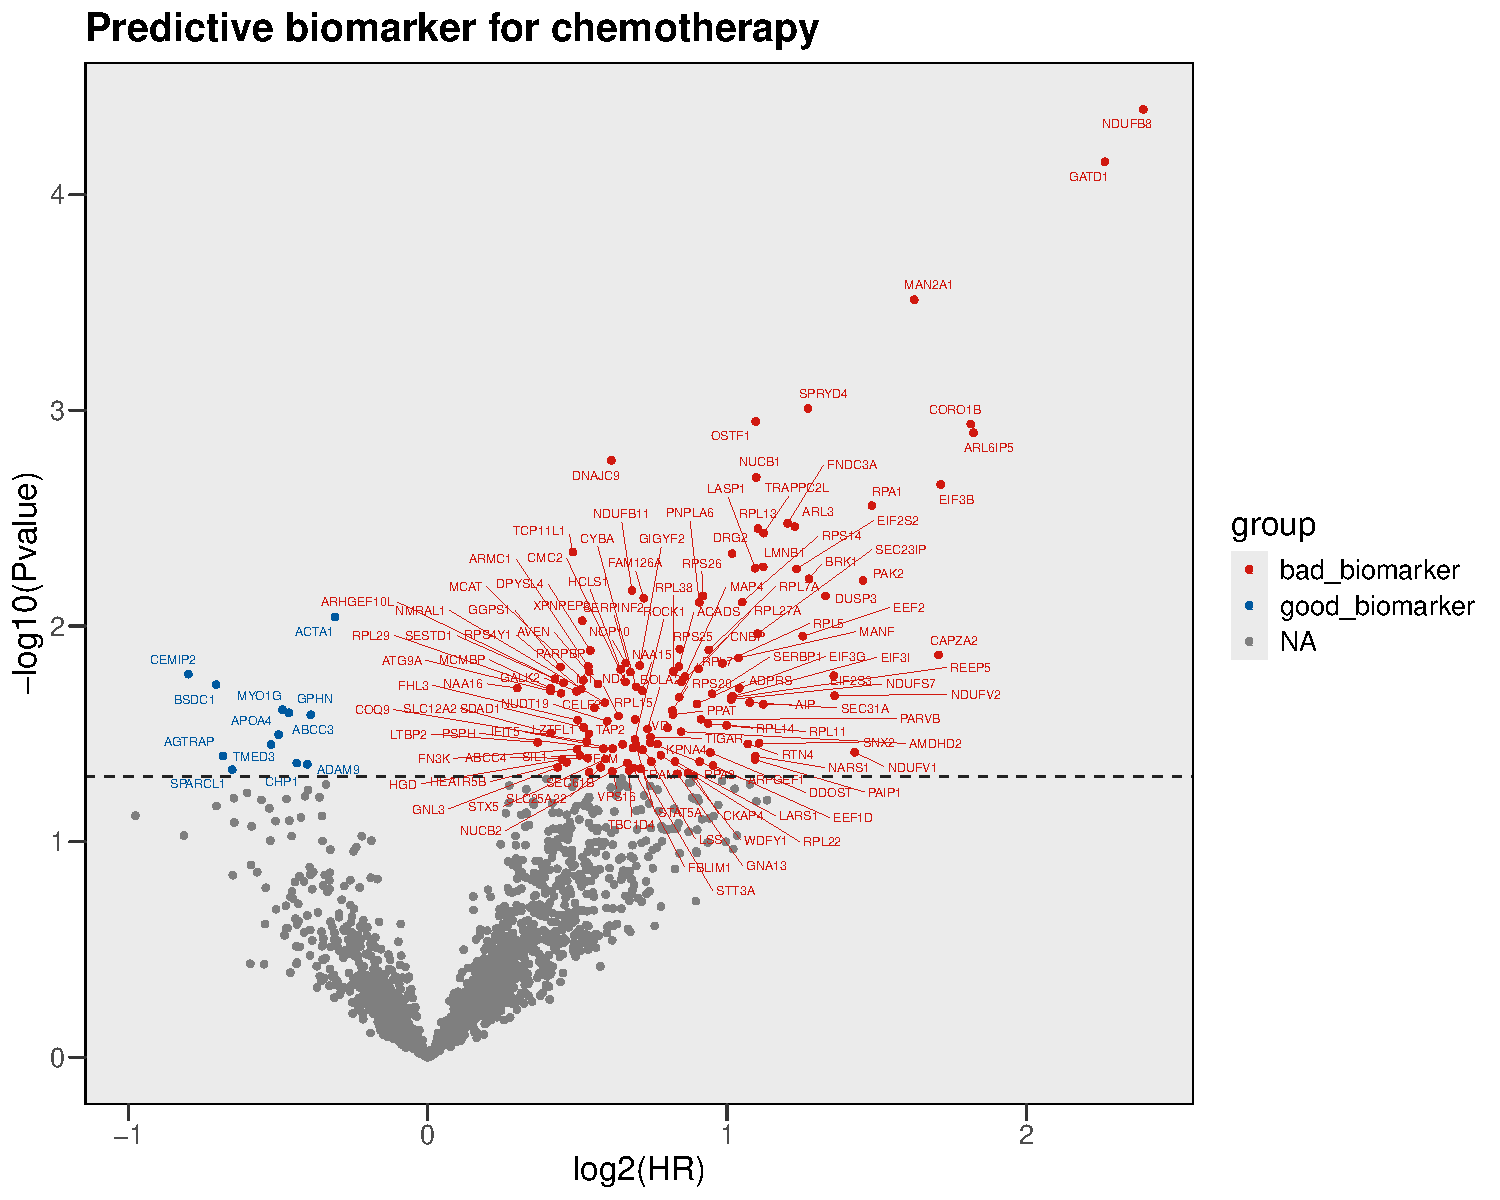
\includegraphics[width=\linewidth]{Figures/4A-Predictive-biomarker.pdf}
          \end{center}
        \end{figure}
    \end{column}

    \begin{column}{0.4\textwidth}
        \begin{figure}
          \begin{center}
            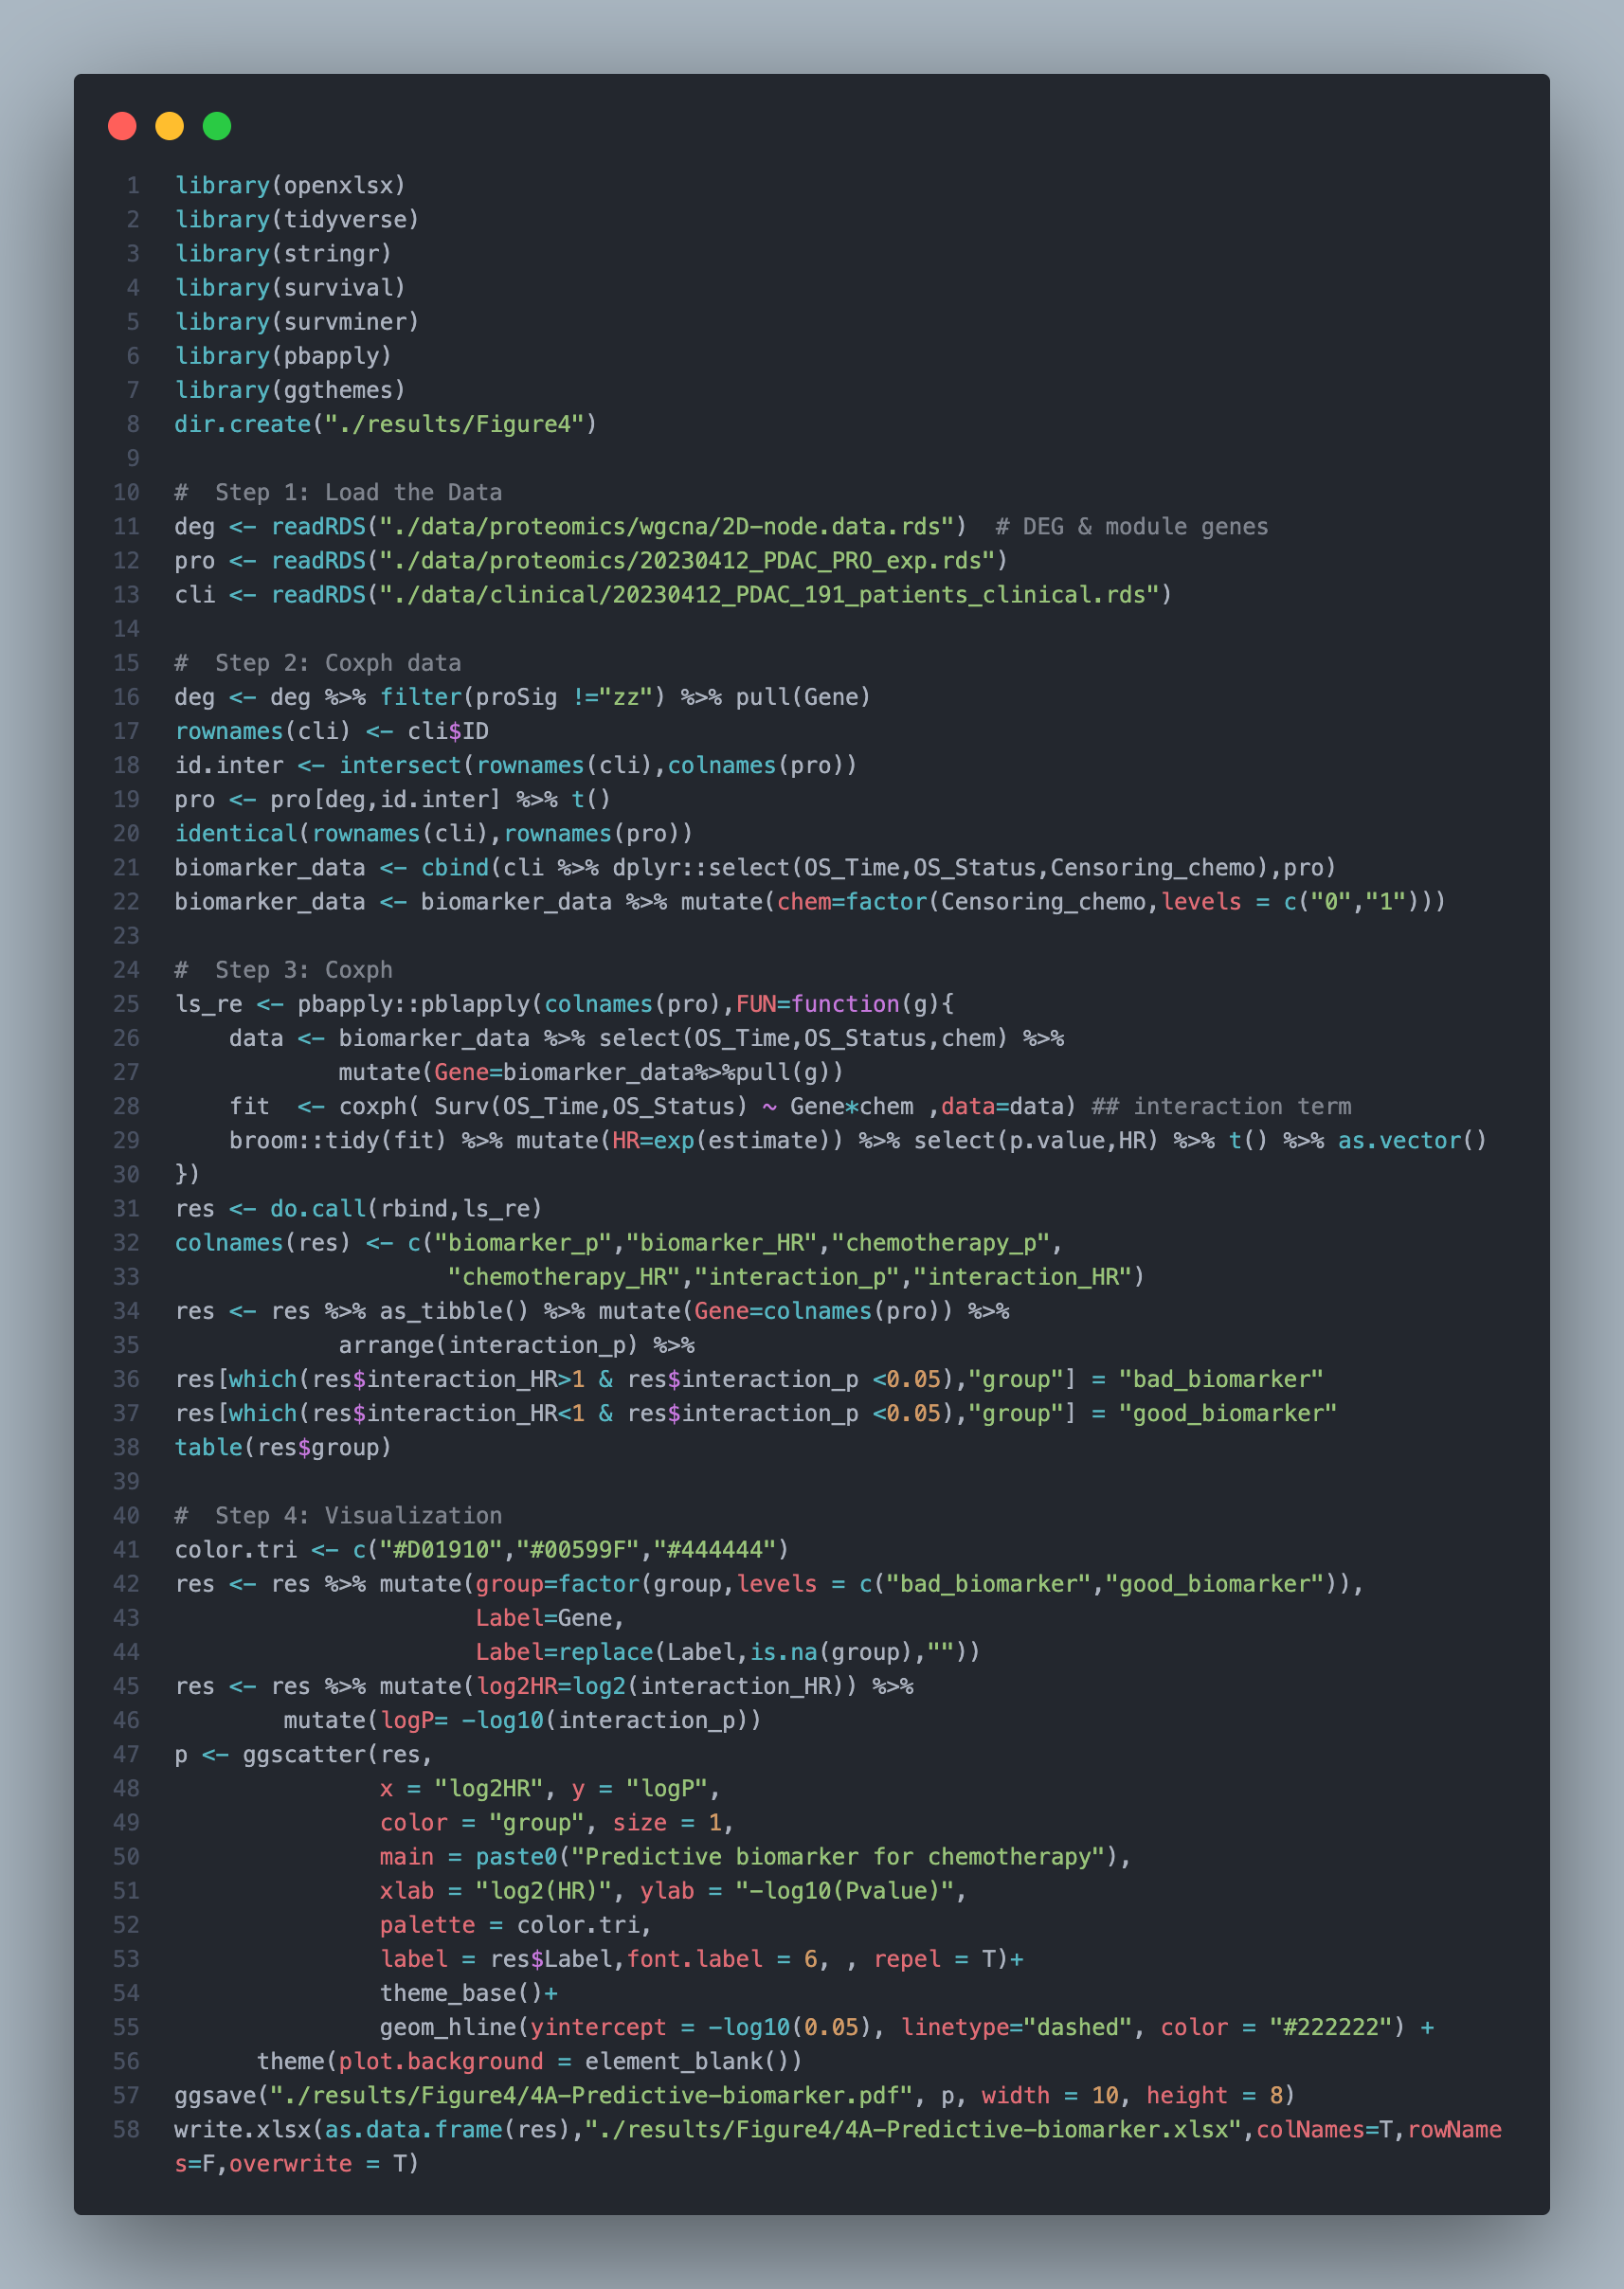
\includegraphics[width=0.8\linewidth]{Figures/4A-Predictive-biomarker-code.png}
          \end{center}
        \end{figure}
    \end{column}
  \end{columns}

  \vspace{0.5cm}
  Scatter plot of the log2 (hazard ratios) versus the -log10 (P-values) of the chemotherapy-by-biomarker interaction term calculated by Cox proportional-hazards models in terms of OS. The blue and red dots represent, respectively, the favorable and unfavorable proteomic biomarkers for adjuvant chemotherapy of PDAC.
\end{frame}

\begin{frame}{Figure \& Code}
  \begin{columns}[onlytextwidth]
    \begin{column}{0.6\textwidth}
        \begin{figure}
          \begin{center}
            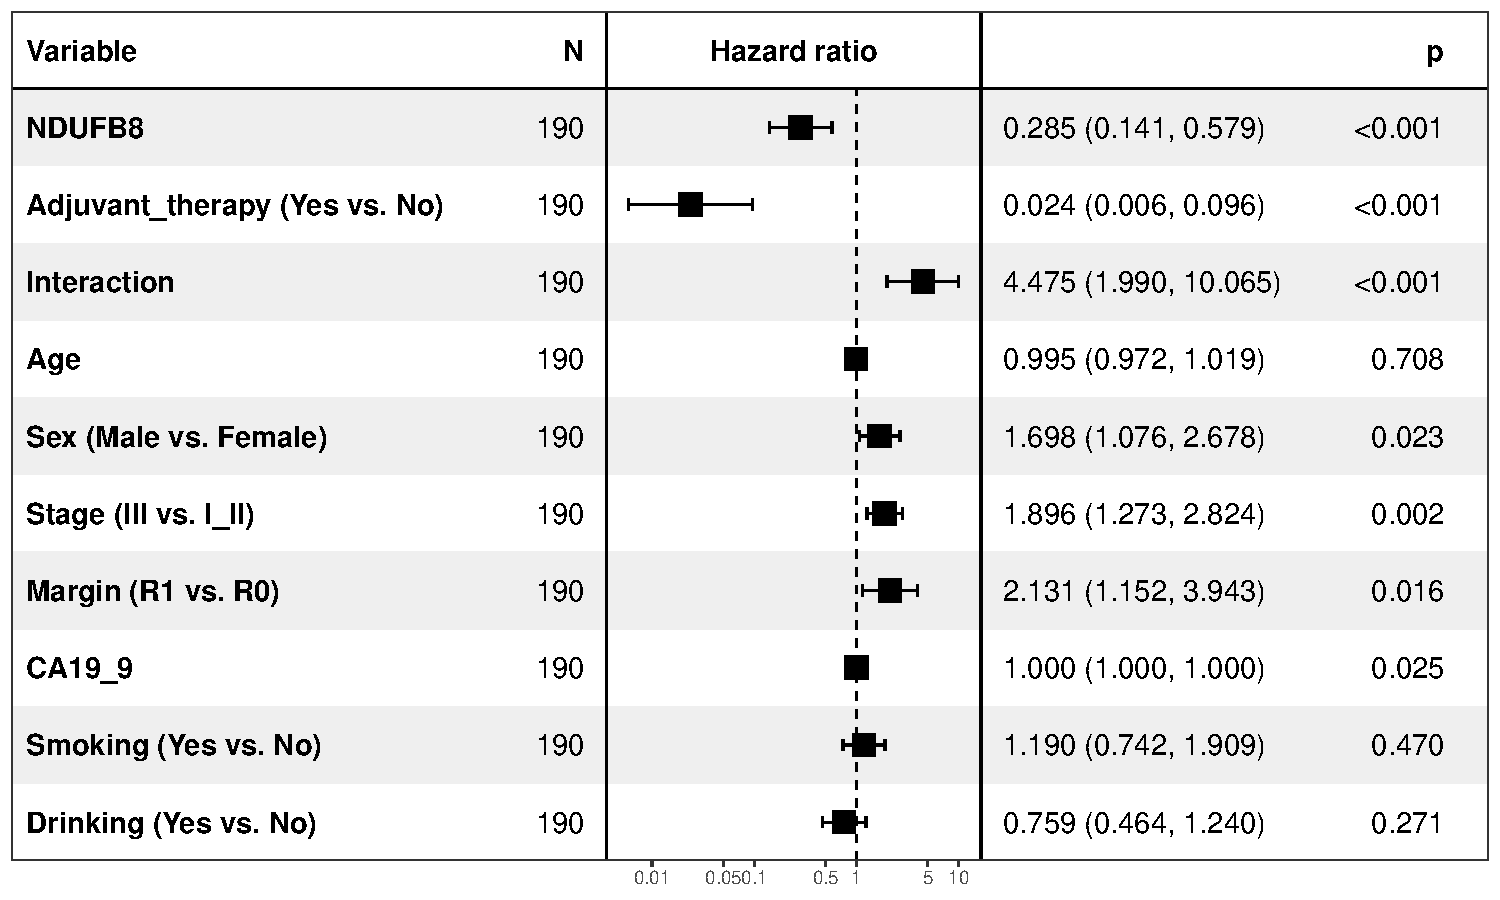
\includegraphics[width=\linewidth]{Figures/Figure4b-1.pdf}
          \end{center}
        \end{figure}
    \end{column}

    \begin{column}{0.4\textwidth}
        \begin{figure}
          \begin{center}
            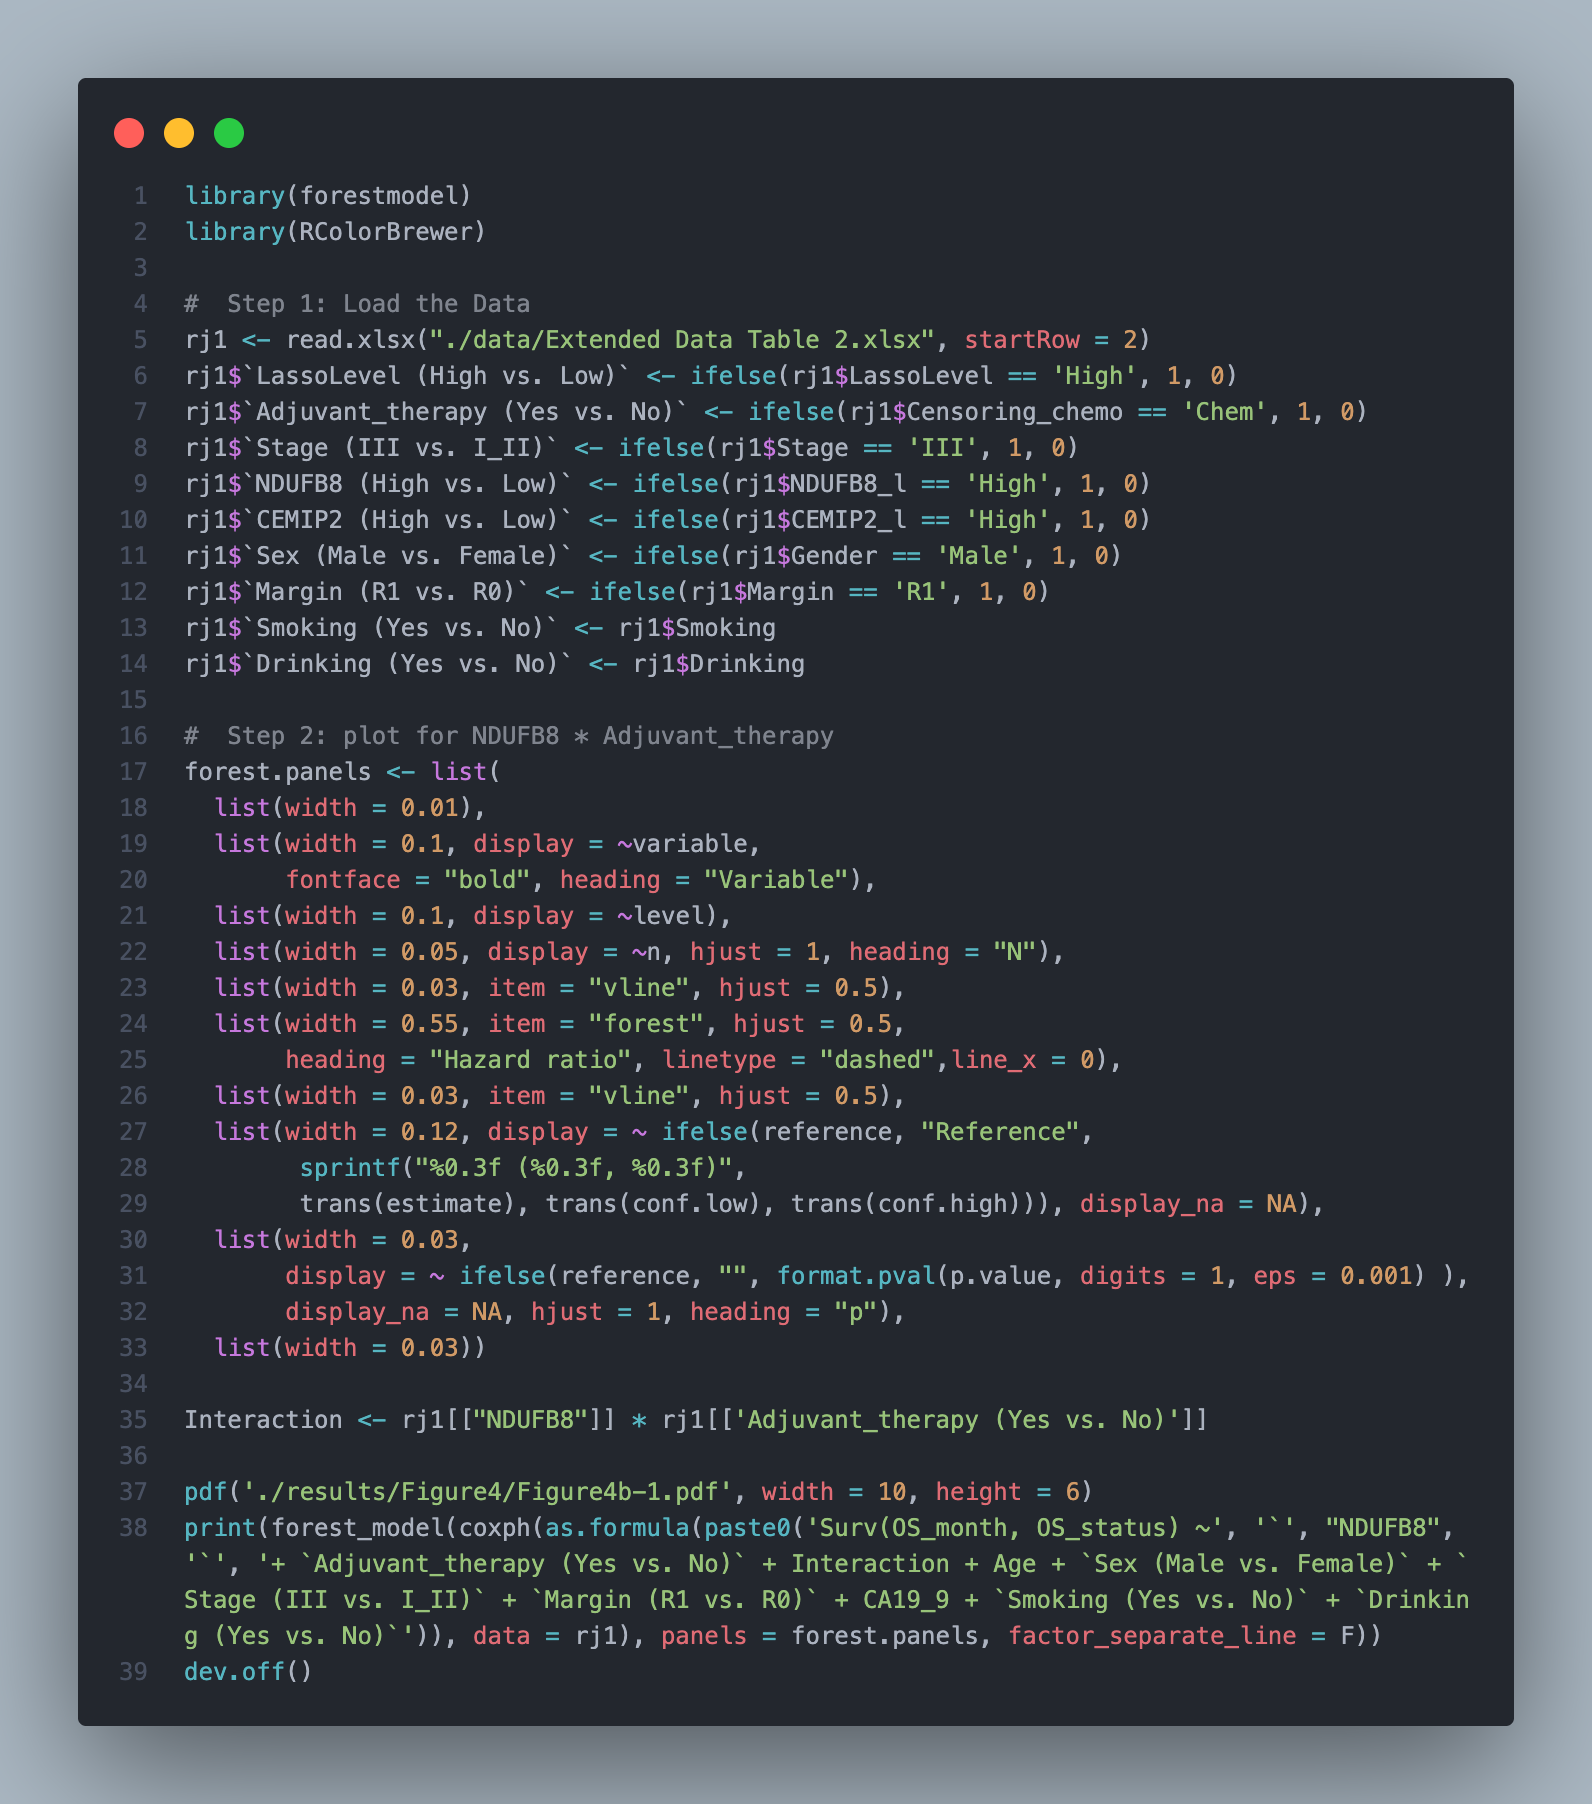
\includegraphics[width=0.8\linewidth]{Figures/Figure4b-1-code.png}
          \end{center}
        \end{figure}
    \end{column}
  \end{columns}

  \vspace{0.5cm}
  Forest plots of multivariable Cox proportional-hazards regression for NDUFB8 and CEMIP2, respectively.
\end{frame}

\begin{frame}{Biomarker validation}
  \begin{itemize}
    \item When NDUFB8 (localized in mitochondria) is highly expressed, chemotherapy shows a clearly better effect.
    \item When CEMIP2 (hyaluronidase) is lowly expressed, chemotherapy also shows good efficacy.
  \end{itemize}
  \begin{figure}
    \begin{center}
      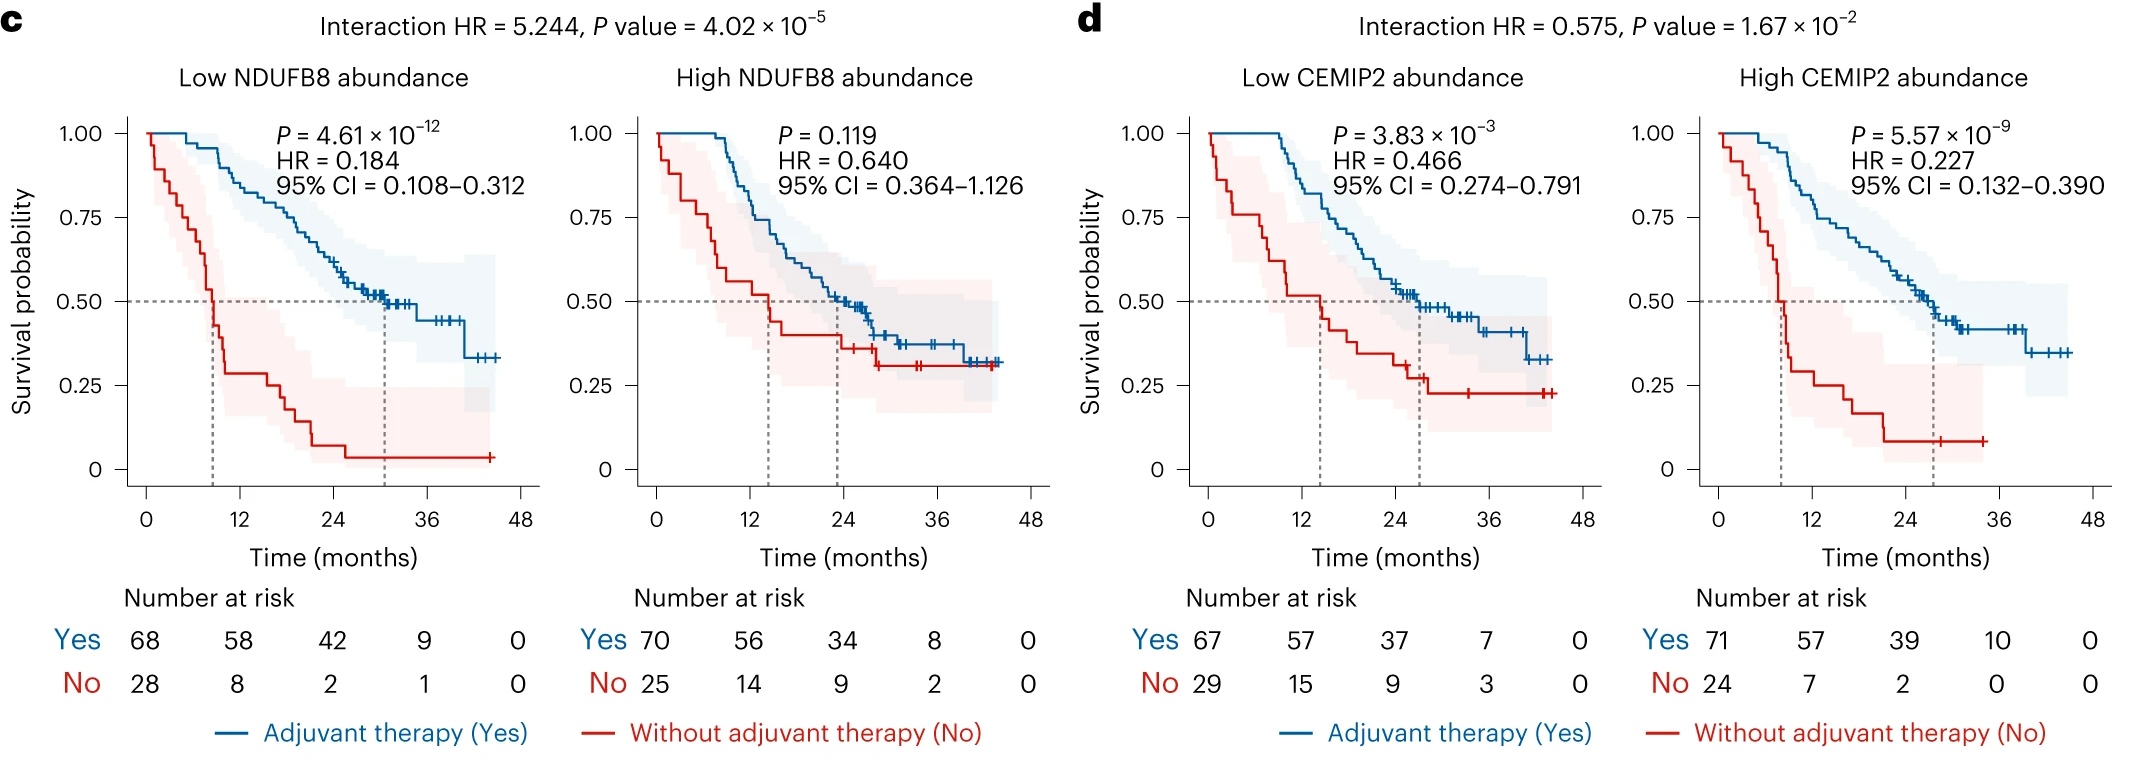
\includegraphics[width=0.85\linewidth]{Figures/Fig4cd.png}
    \end{center}
    \caption{Biomarker validation}
  \end{figure}
\end{frame}

\begin{frame}{Validation across different populations}
  Immunohistochemistry (IHC) was used to directly measure specific protein expression in patients.

  \begin{figure}
    \begin{center}
      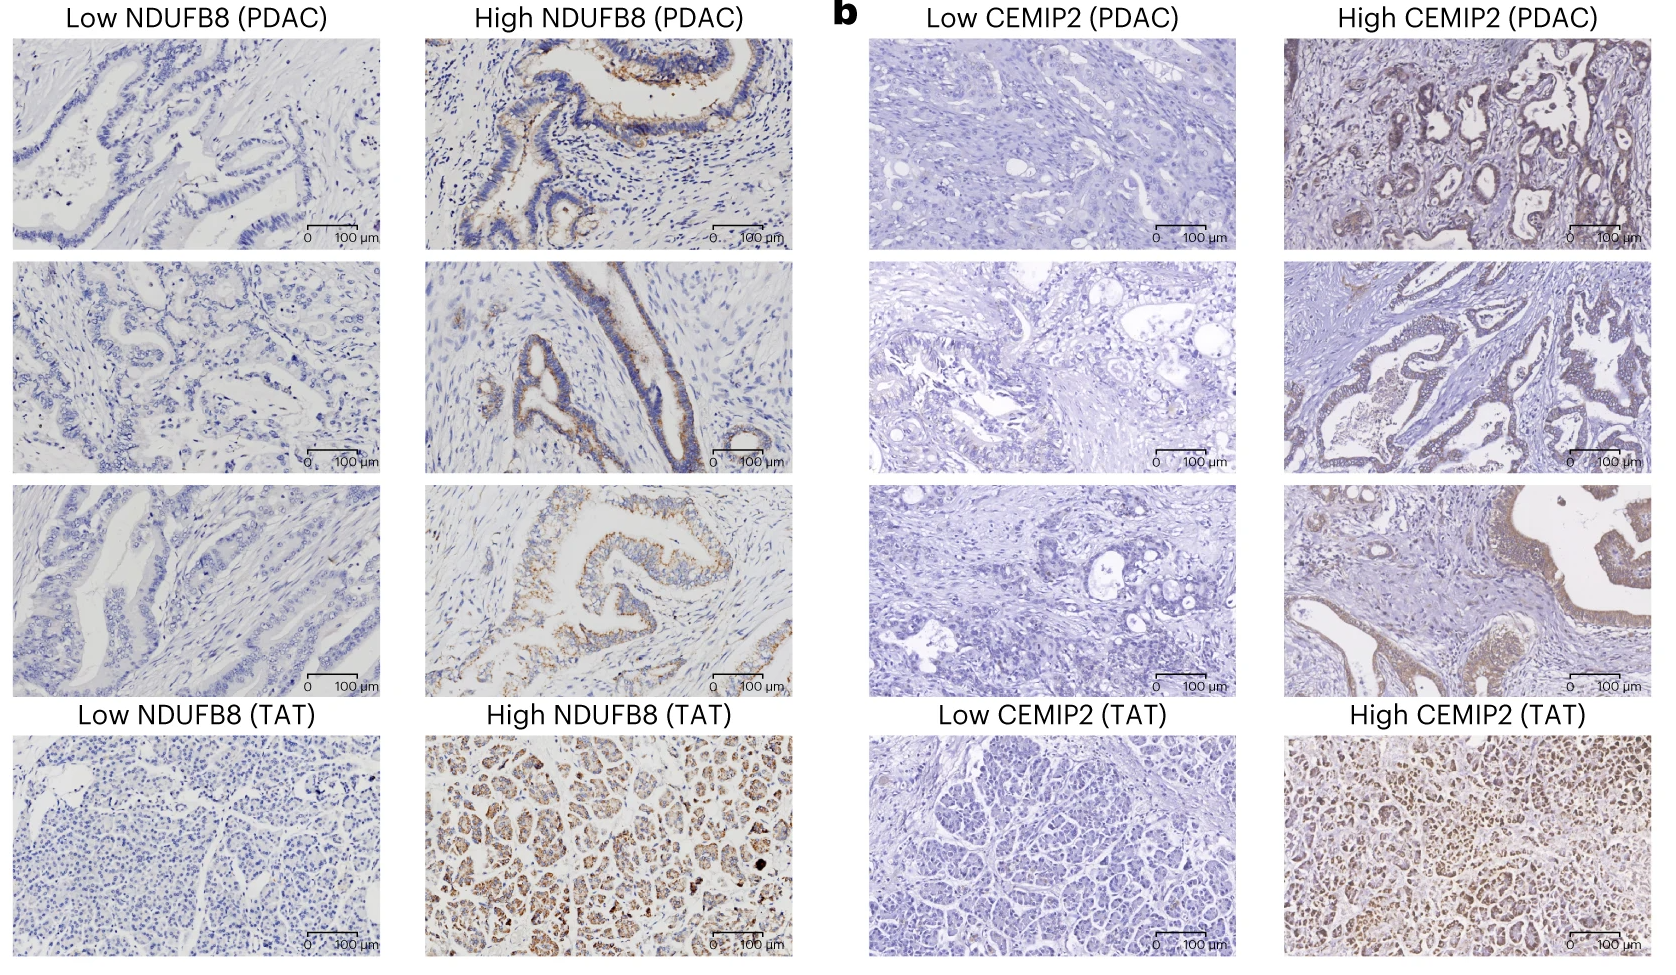
\includegraphics[width=0.8\linewidth]{Figures/Fig5ab.png}
    \end{center}
    \caption{IHC measurement of protein expression}
  \end{figure}
\end{frame}

\begin{frame}{Validation across different populations}
  Patients were grouped by IHC results, and survival curves were re-estimated; the results were fully consistent with the previous findings.

  \begin{figure}
    \begin{center}
      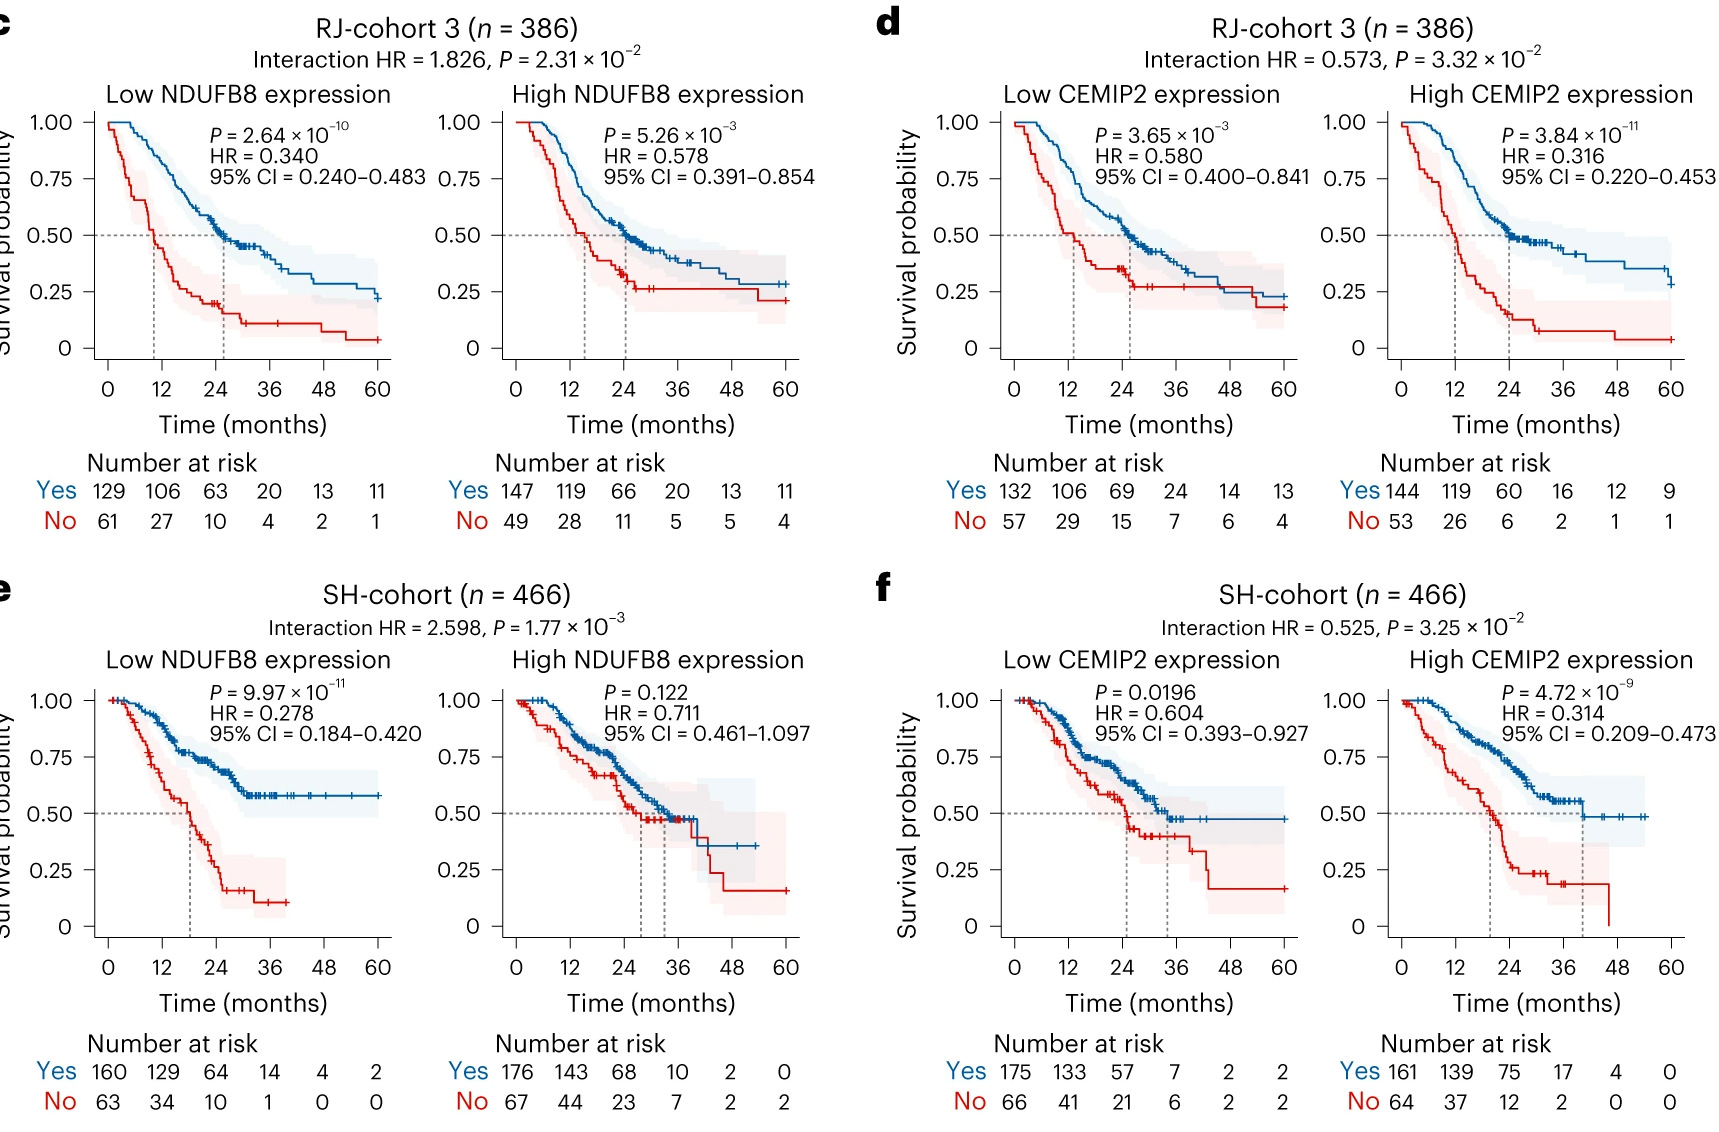
\includegraphics[width=0.7\linewidth]{Figures/Fig5c-h.png}
    \end{center}
    \caption{Cohort validation of biomarkers}
  \end{figure}

\end{frame}

\section{Discussion, Evaluation \& Implication}

\begin{frame}{Bioinformatic tools summary}
  \textbf{Tools used:}
  \begin{itemize}
    \item Proteomics (mass spectrometry): screen proteins.
    \item KM Curve: visualize survival differences.
    \item WGCNA: cluster proteins to facilitate downstream analysis.
    \item LASSO model: select several key proteins via scoring.
    \item Biomarkers: NDUFB8 and CEMIP2.
    \item Multiple validations: internal validation with an alternative method + external multi-center validation to ensure reliability.
  \end{itemize}

\end{frame}

\begin{frame}{Implications: A practical post-surgery stratification framework}
  \begin{block}{Step 1: Prognostic risk (14-protein score)}
    Score-high: higher recurrence risk; consider more intensive treatment and surveillance.
  \end{block}

  \begin{block}{Step 2: Chemo benefit (NDUFB8 and CEMIP2)}
    \begin{itemize}
      \item Low NDUFB8: very large benefit; prioritize treatment completion.
      \item High CEMIP2: stronger benefit; emphasize adherence and access to therapy.
    \end{itemize}
  \end{block}
\end{frame}

\begin{frame}{Limitations and Next steps}
  \begin{itemize}
    \item Observational design: treatment selection and regimen heterogeneity may introduce confounding.
    \item Discovery proteomics subset is moderate in size; multi-center prospective validation is needed.
    \item Open question: are these protein biomarkers universally applicable across the chemotherapy drugs used in practice? 
    \item Toward implementation:
    \begin{itemize}
      \item Standardize assay platform (IHC or small-panel PRM).
      \item Define thresholds and decision rules for reproducible clinical workflows.
      \item Ultimately, biomarker-guided interventional trials are needed.
    \end{itemize}
  \end{itemize}
\end{frame}

\begin{frame}
    \begin{center}
        {\Huge\calligra Thanks!}
    \end{center}
\end{frame}

\end{document}